\documentclass[12pt, oneside,onecolumn,openany]{book}   	% use "amsart" instead of "article" for AMSLaTeX format
\usepackage{geometry}      
\usepackage{blindtext}         
\usepackage[spanish,activeacute]{babel}
\geometry{a4paper}                   		% ... or a4paper or a5paper or ... 
\usepackage{graphicx}	% Use pdf, png, jpg, or eps§ with pdflatex; use eps in DVI mode
\usepackage{subfigure} % subfiguras
\graphicspath{ {images/} }
\usepackage[latin1]{inputenc}			% TeX will automatically convert eps --> pdf in pdflatex		
\usepackage{amssymb}
\usepackage[hyperfootnotes=false]{hyperref}
\usepackage{setspace}
\usepackage{enumerate} 
\usepackage{appendix}
\usepackage{listings}
\spacing{1.5}
\usepackage{wrapfig}
\usepackage{color}
\usepackage{lipsum}
\usepackage{multirow}
\geometry{
 a4paper,
 left=25mm,
 right=20mm,
 top=20mm,
 bottom=20mm
 }

\renewcommand{\appendixname}{Ap�ndices}
\renewcommand{\appendixtocname}{Ap�ndices}
\renewcommand{\appendixpagename}{Ap�ndices}
\renewcommand{\lstlistingname}{}
\newenvironment{bottompar}{\par\vspace*{\fill}}{\clearpage}
%SetFonts

%SetFonts
%listings style
\definecolor{nd}{RGB}{98, 143, 217}
\definecolor{keyword}{RGB}{255,51,102}
\definecolor{bg}{RGB}{255, 255, 232}
\definecolor{comment}{RGB}{73, 79, 92}
\definecolor{str}{RGB}{30, 184, 135}

\lstdefinelanguage{Sass}{
	keywords={mixin, keyframe, include, import, extend, class, \@},
	keywordstyle=\color{keyword},
	indentifierstyle=\color{black}\bfseries,
	sensitive=false,
	comment=[l]{\#},
  	morecomment=[s]{/*}{*/},
    	commentstyle=\color{comment}\ttfamily
}

\lstdefinelanguage{JavaScript}{
 	keywords={typeof, new, true, false, catch, function, return, null, catch, switch, var, if, in, while, do, else, case, break},
  	keywordstyle=\color{keyword},
  	ndkeywords={Router, class, export, boolean, throw, implements, import, this,prototype},
  	ndkeywordstyle=\color{nd}\bfseries,
  	identifierstyle=\color{black},
  	sensitive=false,
  	comment=[l]{//},
  	morecomment=[s]{/*}{*/},
  	commentstyle=\color{comment}\ttfamily,
  	stringstyle=\color{str}\ttfamily,
  	morestring=[b]',
  	morestring=[b]"
}

\lstset{
frame=single,
   language=Javascript,
   backgroundcolor=\color{bg},
   extendedchars=true,
   basicstyle=\small\ttfamily,
   showstringspaces=false,
   showspaces=false,
   numbers=left,
   numberstyle=\footnotesize,
   numbersep=9pt,
   tabsize=2,
   breaklines=true,
   showtabs=false,
   captionpos=b,
   xleftmargin=\parindent,
}

\extrafloats{100}

\title{Trabajo Fin de Grado}
\author{Jorge Ortega Morata}
\date{\today}	
						% Activate to display a given date or no date
\begin{document}
\vspace{2cm}

\begin{figure}[htb]
\centerline{\resizebox{.60\textwidth}{!}{
\includegraphics{images/logo-urjc.jpg}}}
\end{figure}

\begin{center}
{\Large {\bf Grado en Ingenier�a en Tecnolog�as de la Telecomunicaci�n}}
\vspace{5mm}

{\large Escuela T�cnica Superior de Ingenier�a de Telecomunicaci�n}
\vspace{2mm}

{\large Curso acad�mico 2015-2016}

\vspace{0.5cm}

{\large {\bf Trabajo Fin de Grado}} 

\vspace{1.5cm}
\setstretch{2}
{\Huge {PLATAFORMA WEB  PARA 
DESARROLLADORES CON
GRABACIONES DE C�DIGO Y 
AUDIO SOBRE EDITOR COMO 
ELEMENTO FUNDAMENTAL
}}

\end{center}

\vspace{3.2cm}
\makebox[11cm][r]{
\begin{tabular}{ll}
{\bf Autor}: & Jorge Ortega Morata \\
{\bf Tutor}: & Pedro de las Heras Quir�s \\
\end{tabular} 
}

\vspace{0.5cm}
\begin{center}
\large{Madrid 2016}
\end{center}
\thispagestyle{empty}
\clearpage
\begin{bottompar}
\centering
\htmladdnormallink{
\includegraphics[width=2cm]{cc.png}}
      {http://creativecommons.org/licenses/by-nc-nd/4.0/}\\
      \texttt{Aplicaci�n web para desarrolladores basada en la grabaci�n de audio y c�digo sobre editor como elemento fundamental by 
      \href{mailto:j.ortega.morata@gmail.com}{Jorge Ortega Morata}
      is licensed under a \htmladdnormallink{Creative Commons Reconocimiento-NoComercial-SinObraDerivada 4.0 Internacional}
      {http://creativecommons.org/licenses/by-nc-nd/4.0/}}
\end{bottompar}
      
\tableofcontents
\listoffigures

\setstretch{1.2}
\chapter{Resumen}
En el presente trabajo fin de grado se ha realizado la implementaci�n de una aplicaci�n web que sirva de herramienta a desarrolladores de manera que puedan aprender y compartir conocimientos sobre las tecnolog�as de software actuales. 
\\
Se han tenido en cuenta, a la hora de su planificaci�n y concepto, sitios web similares como KhanAcademy y StackExchange 
\paragraph{}
El principal objetivo ha sido crear una herramienta de grabaci�n de c�digo y audio sobre un editor de forma que el elemento b�sico de intercambio de informaci�n en la plataforma fuera lo m�s visual e interactivo posible. Para lograr esa interactividad se ha desarrollado un sistema de respuestas a estos elementos en forma de nuevas grabaciones y la posibilidad de comenzar su grabaci�n en cualquier instante de la reproducci�n de los mismos. Para ello se ha desarrollado un sistema de grabaci�n basado en la sincronizaci�n de audio con eventos capturados sobre un editor de c�digo.
\paragraph{}
Para un correcto desarrollo han sido estudiadas y aplicadas tecnolog�as como WebRTC, MeteorJS, Bootstrap, FlexBox, Javascript, JQuery, SASS, AceEditor, SoundCloud API, MongoDB y HTML5.
\paragraph{}
En este proyecto se ha seguido una metodolog�a basada en SCRUM. El desarrollo de la aplicaci�n se ha dividido en la implementaci�n de distintos prototipos cuyo desarrollo ha servido de base para el siguiente. En cada prototipo se han extra�do requisitos asociados a los principales objetivos propuestos.
\paragraph{}
Una vez finalizada la implementaci�n de la aplicaci�n y realizado su despliegue mediante el sistema de Hosting de Heroku, se ha procedido con la realizaci�n de una prueba de validaci�n basada en la distribuci�n de forma an�nima de una encuesta a alumnos de 4� grado escogidos al azar y con posibilidades de mostrar inter�s por la herramienta desarrollada. Adem�s se ha realizado un estudio de navegaci�n en el sitio gracias a la tecnolog�a de Google Analytics.
\paragraph{}
El an�lisis de los resultados obtenidos ofrece una valoraci�n positiva sobre el flujo de navegaci�n, la funcionalidad, el atractivo, la usabilidad y la acogida del producto conseguido.


%%%%%%%%%%%%%%%%%%%%%%%%%%%%%%%%%%%%%%%%%%%%%%%%%%%%%%%%%%
%%%%%%%                  															       %%%%%%
%%%%%%%                                                     CAPITULO 1:  INTRODUCCI�N                                       %%%%%%
%%%%%%%  																	       %%%%%%
%%%%%%%%%%%%%%%%%%%%%%%%%%%%%%%%%%%%%%%%%%%%%%%%%%%%%%%%%%

\chapter{Introducci�n}
\paragraph{}
Este Trabajo Fin de Grado se desarrolla en el �mbito del desarrollo y tecnolog�as web. En este cap�tulo introduciremos los conceptos y tecnolog�as b�sicas utilizadas y expondremos el paradigma actual en lo que a desarrollo web se refiere.
\section{Desarrollo Web}
\paragraph{}
En la actualidad el desarrollo web se encuentra muy arraigado en nuestra sociedad. Avanza a una velocidad incre�ble, tanto que ni nos percatamos de su impacto en todo lo que nos rodea. Acogemos cada nueva tecnolog�a con los brazos abiertos y al poco transcurso de tiempo desde su primer uso nos es insuficiente. Esa insuficiencia impulsa su crecimiento e impide su decadencia. 
\paragraph{}
Para conocer la historia del desarrollo web es necesario remontarse a los or�genes de \emph{Internet}. En 1969 se crea la primera red de comunicaci�n interconectada entre dos computadoras de dos universidades estadounidenses (UCLA y Stanford) llamada \textbf{ARPAnet}\footnote{https://es.wikipedia.org/wiki/ARPANET} (Advanced Research Projects Agency Network o Red de la Agencia para los Proyectos de Investigaci�n Avanzada de los Estados Unidos) que funcionaba con un protocolo de intercambio de paquetes llamado \textbf{NCP}\footnote{\url{https://en.wikipedia.org/wiki/Network_Control_Program}} (Network Control Program) y que m�s tarde se sustituy� por \textbf{TCP/IP}\footnote{\url{https://es.wikipedia.org/wiki/Modelo_TCP/IP}} por su robustez frente a colisiones. En 1986 comenz� la construcci�n de la primera infraestructura en forma de �rbol de Internet llamada \textbf{NSFNET}\footnote{\url{https://es.wikipedia.org/wiki/NSFNet}} la cual se complement� con otras redes en EEUU. Despu�s se crearon otras redes troncales en Europa y junto con las anteriores ya formaban el \emph{backbone} o red troncal b�sica de Internet. M�s tarde, en 1989 con la creaci�n de la arquitectura de capas OSI en los computadores, comenz� a ser tendencia el utilizar diversos protocolos de comunicaci�n a trav�s de dicha red.  
\paragraph{}
El desarrollo web se inici� con la propia web o lo que conocemos como \textbf{WorldWideWeb}\footnote{\url{https://es.wikipedia.org/wiki/World_Wide_Web}} (WWW) que fue el primer cliente web creado por el \emph{CERN}, cuyo equipo tambi�n cre� el lenguaje \emph{HTML}\footnote{\url{https://es.wikipedia.org/wiki/HTML}} (HyperText Markup Language). Lenguaje b�sico a la hora de estructurar la informaci�n en un sitio web.
\paragraph{}
El desarrollo web comprende todo el proceso de creaci�n de un sitio web. La elecci�n de las herramientas a utilizar, de dise�o y desarrollo, qu� metodolog�a seguir, prototipado, propuesta final y lanzamiento. Es una labor compleja transformar una idea en algo f�sico y dotarla de utilidad para la sociedad. Es un reto que yo, como alumno, nunca hab�a tenido la oportunidad de afrontar y me alegro de haber tenido la ocasi�n de realizar este proyecto.
\paragraph{}
La labor del desarrollador web en la actualidad es mucho m�s sencilla y accesible gracias a las tecnolog�as que surgen cada pocas semanas o d�as. Con el t�rmino \emph{open source} en auge, millones de usuarios de Internet quieren aportar su granito de arena a esta labor y propician un crecimiento en herramientas web incre�ble y en ocasiones vertiginoso. 
\section{Tecnolog�as Web}
Entran en este �mbito todas aquellas herramientas creadas espec�ficamente para generar contenido web. Seg�n su finalidad dentro del desarrollo web podemos diferenciarlas en Frameworks, librer�as y lenguajes.
\paragraph{}
\subsection{Frameworks}
Seg�n su definici�n un \textbf{framework}\footnote{\url{https://es.wikipedia.org/wiki/Framework}} es un \emph{conjunto de conceptos y pr�cticas estandarizados} dise�ado para afrontar un problema en particular, en este caso, el proporcionar una \emph{infraestructura de software} a la hora de crear una aplicaci�n web. Al usar un framework debemos seguir una serie de reglas establecidas seg�n su dise�o a la hora de organizar el c�digo. Hoy en d�a estamos siendo testigos de la \emph{"Batalla de los frameworks"} en lo que a desarrollo web se refiere y es que su crecimiento y potencial es incre�ble. Es muy importante conocer los puntos fuertes y d�biles de cada uno de ellos a la hora de dise�ar una aplicaci�n ya que no todos incorporan los mismos conceptos y pr�cticas. Adem�s tambi�n es imprescindible entender el \emph{entorno de ejecuci�n} de cada uno de ellos a saber: cliente (\textbf{Front-End]}), servidor (\textbf{Back-End})\footnote{\url{https://es.wikipedia.org/wiki/Front-end_y_back-end}} o ambos (\textbf{Full Stack}).

\paragraph{}
En la actualidad se utilizan numerosos frameworks entre los que destacan: \textbf{AngularJS}\footnote{\url{https://angularjs.org/}}, \textbf{EmberJS}\footnote{\url{http://emberjs.com/}}, \textbf{Django}\footnote{\url{https://www.djangoproject.com/}}, \textbf{ReactJS}\footnote{https://facebook.github.io/react/}, \textbf{MeteorJS}\cite{baz5}, \textbf{BackboneJS}\footnote{\url{http://backbonejs.org/}} y \textbf{ExpressJS}\footnote{\url{http://expressjs.com/es/}}. Todos utilizan \emph{Javascript}\footnote{\url{https://es.wikipedia.org/wiki/JavaScript}} como lenguaje de desarrollo a excepci�n de Django que utiliza \emph{Python}\footnote{\url{https://www.python.org/}}. 

\subsubsection{AngularJS}
\paragraph{}
Es un framework front-end. Hace posible realizar peticiones REST y se pueden desarrollar \emph{proveedores} que brindan servicios al cliente que se encuentran en el lado del servidor. La principal caracter�stica de Angular es que mediante su concepto de \emph{directiva} podemos construir toda la aplicaci�n de forma modular. Adem�s cuenta con \emph{two data-binding }que permiten el \emph{renderizado reactivo} y din�mico de sus plantillas o m�dulos.
\paragraph{}
AngularJS es una creaci�n de Google y es el framework m�s utilizado hoy en d�a, por lo que posee una gran comunidad, y uno de los m�s pesados en lo que respecta a tama�o.
\subsubsection{EmberJS}
\paragraph{}
Se trata de un framework front-end muy potente dise�ado para crear aplicaciones grandes. Mediante la librer�a \textbf{Handlebars} \footnote{\url{http://handlebarsjs.com/}} que incorpora podremos crear plantillas din�micas gracias al \emph{data-binding} que presenta. Adem�s tambi�n posee un \emph{CLI} (Interfaz de L�nea de Comandos) que nos permitir� configurar todo mediante comandos. Posee el m�dulo de \emph{routing} m�s avanzado de todos los frameworks. Es una excelente herramienta para desarrollar un cliente con un buen nivel de potencial.
\subsubsection{Django}
\paragraph{}
Django, al igual que Ruby on Rails o MeteorJS no se deber�a de considerar framework sino \emph{plataforma} de desarrollo web, ya que es full-stack y posee su propio CLI. El lenguaje de desarrollo es Python. Posee todas las herramientas necesarias para generar un servidor y un cliente. Es una herramienta muy completa. En el momento de su lanzamiento experiment� una gran acogida y a�n conserva su fama tras sus numerosas actualizaciones.
\subsubsection{ReactJS}
\paragraph{}
Este es el framework m�s limitado en lo que a �mbito de ejecuci�n se refiere (desarrollo de  las vistas en el cliente y poco m�s). Pero es incre�blemente \emph{flexible}. La forma en la que se crean las plantillas en ReactJS (sin necesidad de escribir HTML) es incre�ble. Ha sido creado por Facebook y se utiliza cada vez m�s por su concepto de reactividad.
\subsubsection{MeteorJS}
\paragraph{}
MeteorJS \cite{baz5}, como dec�amos de Django, se le deber�a tratar como una plataforma de desarrollo. Corre sobre \textbf{NodeJS}\footnote{\url{https://nodejs.org/en/}} y la principal ventaja que ofrece es que el servidor es completamente transparente al desarrollador. Solo debe preocuparse de crear el modelo de datos (m�s bien enunciarlo porque cuenta con \textbf{MongoDB}\cite{baz10} como base de datos), las rutas, las \emph{publicaciones} de datos reactivos y de las plantillas de la aplicaci�n. Ha sido el pionero en lo que respecta al concepto de \emph{reactividad} antes que ReactJS. Es una herramienta a tener en cuenta por su gran comunidad y sus paquetes espec�ficos y por su capacidad para el \emph{prototipado} r�pido.
\paragraph{}
Exploraremos m�s a fondo las caracter�sticas de este framework m�s adelante ya que es el framework elegido para el desarrollo de nuestra aplicaci�n que es de lo que trata este proyecto.
\subsubsection{BackboneJS}
\paragraph{}Se trata de otro de los frameworks front-end m�s usados en la actualidad y no es de extra�ar debido a su sencillez y capacidad. Es ideal para aplicaciones peque�as y medianas.
\subsubsection{ExpressJS}
\paragraph{}
Este es un framework back-end y permite crear un servidor NodeJS en pocos minutos para s�lo preocuparse del desarrollo front-end. Actualmente tiene cabida en cualquier proyecto por su f�cil integraci�n con cualquiera de los frameworks front-end.
\subsubsection{Bootstrap \cite{baz8}}
\paragraph{}
Es m�s una \emph{librer�a} que un framework pero dado que posee un paradigma especial y unas reglas claras a la hora de usarlo se le considera un framework front-end. Permite el dotar a tu aplicaci�n de estilo r�pidamente puesto que ya tiene definidos estilos por defecto, y crear m�dulos funcionales para organizar el contenido, adem�s de animaciones. Est� destinado a la labor de maquetaci�n y es el m�s utilizado hoy en d�a. Aunque tambi�n se utilizan otros como \textbf{Foundation} \footnote{\url{http://foundation.zurb.com/}} o \textbf{Pure} \footnote{\url{http://purecss.io/}} que tambi�n poseen buenas caracter�sticas para dicha labor.

\subsection{Librer�as}
\paragraph{}
Las librer�as son un \emph{conjunto de utilidades programadas} en un lenguaje dado que proporcionan un \emph{servicio concreto} al desarrollador. Al contrario que un programa no est�n pensadas para un uso autom�tico, es decir, no tienen un inicio. S�lo son usadas por programas. En lo que se refiere a desarrollo web son utilizadas para aportar servicios al desarrollador de la aplicaci�n. La librer�a l�der en este �mbito es \textbf{JQuery}\cite{baz11}\cite{baz12} y sus descendientes como \textbf{JQueryUI} \footnote{\url{https://jqueryui.com/}}. Otra liber�a cada vez m�s utilizada es \textbf{UnderscoreJS}.
\subsubsection{JQuery}
\paragraph{}
Se trata de una librer�a que permite manipular el \emph{DOM}\footnote{\url{https://es.wikipedia.org/wiki/Document_Object_Model}} (Document Object Model) desde la l�gica de la aplicaci�n. No necesitamos hacer uso del objeto document para realizar b�squedas, a�adir etiquetas y dem�s operaciones de manipulaci�n. Mediante JQuery podremos establecer eventos, manipular din�micamente el DOM a�adiendo etiquetas y estilos y mucho m�s. Es una herramienta indispensable para el desarrollador web. Lo es tanto que incluso otras librer�as y paquetes destinados a diferentes frameworks la usan.
\subsubsection{UnderscoreJS \cite{baz13}}
\paragraph{}
Esta es una librer�a que permite manipular objetos, colecciones de objetos y arrays. Permite realizar \emph{operaciones de filtrado} muy avanzadas sobre una colecci�n de objetos y adem�s realizar iteraciones de forma funcional mediante sus m�todos 


\subsection{Lenguajes}
\paragraph{}
Existen numerosos lenguajes en desarrollo web: \textbf{Java} (para servidores principalmente), \textbf{Javascript}, \textbf{CoffeeScript}, \textbf{TypeScript}, \textbf{HTML5}, \textbf{Jade}, \textbf{CSS}, \textbf{Less}, \textbf{Sass}, \textbf{Python}, \textbf{Ruby}, etc. Pero hay que tener en cuenta que lo que el navegador compila e interpreta son ficheros CSS, HTML y lenguajes de l�gica de la aplicaci�n como Javascript. Por lo que si desarrollamos con Jade, Less, Sass, CoffeeScript o TypeScript debemos de preprocesarlos hacia los tres principales lenguajes mencionados anteriormente.
\subsubsection{HTML5}
\paragraph{}
Se trata de la quinta versi�n del lenguaje HTML. Posee una variante de sintaxis b�sica conocida como HTML5 y otra \textbf{XHTML} conocida como XHTML5 y se sirve como sintaxis \textbf{XML} \footnote{\url{http://www.w3schools.com/xml/}} (eXtensible Markup Language) concebido por el \textbf{World Wide Web Consortium} \footnote{\url{https://es.wikipedia.org/wiki/World_Wide_Web_Consortium}}(W3C) con el fin de almacenar datos de forma legible y que complementa en la mayor�a de aplicaciones al documento HTML. 
\paragraph{}
En esta quinta versi�n se han desarrollado nuevas etiquetas que ayudan a realizar un documento m�s sem�ntico y legible, adem�s de proporcionarnos herramientas de dibujo en 2D y 3D, etiquetas para introducir audio y video o de formato. Etiquetas como: \emph{$<$article$>$}, \emph{$<$aside$>$},\emph{ $<$audio$>$}, \emph{$<$video$>$}, \emph{$<$canvas$>$}, \emph{$<$datalist$>$}, \emph{$<$details$>$}, \emph{$<$dialog$>$}, \emph{$<$embed$>$}, \emph{$<$figure$>$}, \emph{$<$footer$>$}, \emph{$<$header$>$}, \emph{$<$mark$>$}, \emph{$<$meter$>$}, \emph{$<$nav$>$}, \emph{$<$output$>$}, \emph{$<$progress$>$}, \emph{$<$ruby$>$}, \emph{$<$rp$>$}, \emph{$<$rt$>$}, \emph{$<$section$>$}, \emph{$<$source$>$} y \emph{$<$time$>$}. 
\paragraph{}
Tambi�n incorpora herramientas nuevas como un visor de f�rmulas matem�ticas (\textbf{MathML}), tecnolog�a \textbf{Drag \& Drop} (arrastrar y soltar objetos basado en eventos), ejecuci�n en paralelo mediante \textbf{WebWorkers}, comunicaci�n bidireccional entre p�ginas mediante \textbf{WebSockets}, \textbf{APIs} para almacenamiento (\textbf{Local \& Global Storage}), \textbf{geolocalicaci�n} y para trabajar sin conexi�n (\textbf{Off-line}).
\paragraph{}
La incorporaci�n de estas nuevas herramientas reduce la necesidad del desarrollador a utilizar \emph{plugins} externos.
\subsubsection{CSS3}
\paragraph{}
CSS es el lenguaje utilizado para crear la presentaci�n y dar estilo al documento HTML o XML. En esta tercera versi�n se introducen nuevas funcionalidades como animaciones 3D, transiciones, estructuraci�n mediante propiedades \emph{grid} (rejilla), \emph{media querys} para establecer cambios de estilo conforme el tama�o de la pantalla var�a, etc.
\subsubsection{Javascript \cite{baz9}}
\paragraph{}
Es el lenguaje de programaci�n m�s usado hoy en d�a en el desarrollo web (sobretodo en el lado del cliente). Fue creado por \emph{Brendan Eich} de \textbf{Netscape} como dialecto de \textbf{ECMAScript} \footnote{\url{https://en.wikipedia.org/wiki/ECMAScript}}. Su primer nombre fue \emph{Mocha}, despu�s \emph{LiveScript} y finalmente Javascript. Es un lenguaje orientado a objetos, basado en \textbf{prototipos}, funcional (las funciones son objetos), posee un \emph{tipado} muy d�bil y es din�mico. 
\paragraph{}
Como se ha comentado, el marco de utilizaci�n de este lenguaje en el desarrollo web son los frameworks front-end. Aunque tambi�n se utilizan frameworks basados en NodeJS o el propio NodeJS para desarrollar mediante este lenguaje en el lado del servidor en numerosos proyectos. 
\paragraph{}
Javascript sigue creciendo y actualiz�ndose. En 2015 fue lanzado el est�ndar \textbf{ECMAScript6} \footnote{\url{http://www.campusmvp.es/recursos/post/ECMAScript-6-es-ya-un-estandar-cerrado.aspx}}, el cual dota a javascript de nuevas funcionalidades y m�dulos como un nuevo paradigma de orientaci�n a objetos basado en \textbf{clases}, iteradores o \textbf{promesas} para programaci�n as�ncrona.
\section{MeteorJS}
\paragraph{}
Meteor es una \emph{plataforma} que permite crear aplicaciones Web en \emph{tiempo real} basada en \textbf{NodeJS}. Fue creado con el prop�sito del \emph{prototipado r�pido} y en este �mbito supera a la mayor�a de \emph{frameworks}. Ha sido el primero en introducir el principio de \emph{reactividad} en el desarrollo web. Soporta \textbf{MongoDB} como tecnolog�a de base de datos y posee un asombroso concepto de \emph{subscripciones} a \emph{publicaciones} procedentes de \emph{colecciones} que hacen del \emph{renderizado} del \textbf{DOM} un proceso muy r�pido gracias a que mantiene en el cliente una mini base de datos llamada \emph{MiniMongo}. El cliente es capaz de modificar dicha base de datos y observar los cambios directamente que m�s tarde se actualizar�n en la base de datos del servidor.

\subsection{Reactividad}
\paragraph{}
EL gran potencial de Meteor es debido a este \emph{principio}. Se basa en observar los cambios sobre una \emph{fuente} en tiempo real y actuar en consecuencia, dotando a las aplicaciones de un \emph{dinamismo} muy especial. Adi�s a los \emph{Listeners} y al \emph{binding} sobre elementos \textbf{HTML}, no hacen falta si sabes aprovechar este principio y sus \emph{entidades}.
En meteor existen numerosas entidades que proveen \emph{reactividad} y otras muchas que permiten crear nuevas \emph{entidades reactivas}. Las \textbf{fuentes reactivas} que puedes controlar de manera simple en Meteor son las \emph{variables de sesi�n} almacenadas en \emph{Session}. Mediante la sentencia \emph{Session.set(key[String],value)} ya tienes una fuente reactiva a tu disposici�n. S�lo necesitas algo que sepa escuchar sus cambios y actuar (\emph{helpers} o \emph{Tracker}). 
\paragraph{}
El modulo \textbf{Tracker} posee un m�todo \emph{.autorun()} que permite ejecutar c�digo cuando una fuente reactiva cambia. Adem�s puede directamente asociarse a la l�gica de cualquier plantilla dentro del m�todo \emph{.rendered()} del controlador. Esto permite dotar a la plantilla de dinamismo, por ejemplo realizar \textbf{subscripciones din�micas} sobre una colecci�n enlazado con los eventos de la plantilla. (Autocompletados basados en subscripciones, Botones para cargar m�s contenido, etc).
\subsection{Sistema de plantillas reactivas}
\paragraph{}
 Meteor utiliza una \emph{biblioteca} muy poderosa para crear \emph{interfaces de usuario} que se actualizan en tiempo real
llamada \textbf{Blaze} \footnote{\url{https://guide.meteor.com/blaze.html}}. Cumple el mismo prop�sito que \textbf{Angular}, \textbf{Backbone}, \textbf{Ember}, \textbf{React}, \textbf{Polymer} o \textbf{Knockout} en este �mbito
pero es mucho m�s sencilla de utilizar, incluso \emph{transparente} para el programador. Su labor no ser�a posible sin 
\emph{Tracker}, un m�dulo de Meteor que permite gestionar \emph{procesos reactivos} de manera limpia, y sin \textbf{Spacebars} \footnote{\url{http://meteorcapture.com/spacebars/}} 
(parecido a \textbf{Handlebars}), el lenguaje particular de Meteor para definir las plantillas y que aprovecha al m�ximo la funcionalidad
de \emph{Tracker}.
\subsection{Comunicaci�n con el servidor}
\paragraph{}
La comunicaci�n con el servidor se basa en el protocolo HTTP que Meteor integra de manera transparente al programador mediante su m�dulo \emph{methods} al que se accede mediante \emph{Meteor.methods()} y para la petici�n de recursos se utiliza alg�n paquete creador de rutas como \textbf{IronRouter}\cite{bazIronRouter} o \textbf{FlowRouter} \footnote{\url{https://github.com/kadirahq/flow-router}}. Tambi�n posee el m�dulo \emph{http} para realizar peticiones desde el cliente al servidor y a terceros. Todas las peticiones son as�ncronas y como tales se les asocian callbacks (funciones que se ejecutar�n una vez haya terminado la ejecuci�n de la petici�n).
\paragraph{}
Cada vez que se define una plantilla mediante Spacebars se crea un objeto plantilla Template.name y que lo tendremos accesible a la hora de dotarla de funcionalidad mediante javascript. Es un tipo de controlador. Spacebars permite el paso de datos de la plantilla al controlador y viceversa, esto se denomina \textbf{two data-binding} y supone una poderosa herramienta a la hora de crear componentes aislados puesto que su configuraci�n puede realizarse v�a Spacebars. Este proceso lo realiza mediante la declaraci�n de helpers o ayudantes de plantilla y se definen mediante la funci�n \emph{helpers()} del controlador. La gran ventaja de esto radica en que los helpers son funciones javascript asociadas a una fuente reactiva. Esto quiere decir que en el momento que esa fuente cambia los helpers se actualizan y se actualiza el contenido HTML asociado a ellos. Adem�s de permitir crear componentes reusables, �stos son din�micos (reactivos) en su instanciaci�n y durante su uso.
\paragraph{}
Aparte de los helpers al controlador se le puede asociar un mapa de eventos relacionados con la plantilla mediante la funci�n \emph{events()} que toma como par�metro un objeto javascript cuyos m�todos definir�n las funciones de los mismos.
\subsubsection{Jerarqu�a de carpetas y orden de carga}

\paragraph{}
Para aplicaciones peque�as es posible escribir el c�digo ejecutable por el cliente y por el servidor en una misma carpeta. Para ello Meteor cuenta con las funciones \emph{.isClient()} y .\emph{isServer()} para especificar qu� c�digo debe ejecutarse en cada entorno. Para aplicaciones m�s grandes la estructura es un poco peculiar y se debe generar teniendo en cuenta el orden de carga seg�n la \emph{jerarqu�a de carpetas}. Este orden de carga aunque sea muy estricto provee de una flexibilidad asombrosa y permite crear cualquier aplicaci�n de forma \emph{modular}. La jerarqu�a de carpetas ser�a la siguiente:
\begin{figure}[h]
    \centering
    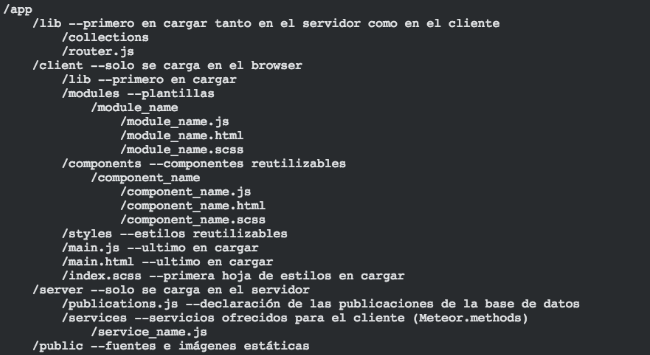
\includegraphics[width=1\textwidth]{hierarchyFolders.png}
    \caption{jerarqu�a de carpetas}
    \label{fig:hierarchyFolders}
\end{figure}

\paragraph{}
La carpeta \emph{/lib} de m�s alto nivel dentro de la jerarqu�a contiene todos los \emph{ficheros comunes} a ambos entornos (cliente y servidor) y es la primera en cargar. \emph{/server} y \emph{/client} contienen todos los \emph{ficheros ejecutables} por el servidor y por el cliente respectivamente. Dentro de cada una de las carpetas anteriores existe un orden de carga. Si poseen carpeta \emph{/lib} ser� la primera en cargar, despu�s es el turno de los dem�s ficheros en \emph{orden alfab�tico} y, por �ltimo, los ficheros \emph{main.*} sea cual sea su extensi�n. En la carpeta \emph{/public} se encuentra el \emph{contenido est�tico} de nuestra aplicaci�n (fuentes, im�genes, etc).

\paragraph{}
Como podemos ver seg�n el orden y �mbito de ejecuci�n Meteor ofrece un \emph{entorno de ejecuci�n sim�trico} (se ejecuta tanto en el cliente como en el servidor) dentro de la carpeta \emph{/lib} de m�s alto nivel en la jerarqu�a. La principal ventaja de esto es que no tenemos porqu� replicar c�digo. Podemos crear \emph{constructores} y dem�s funcionalidad necesaria en ambos entornos una sola vez y Meteor se encarga de saber que cargar en cada uno.
\paragraph{}
Adem�s, al ser MeteorJS una plataforma de desarrollo, no es necesario un \emph{gestor de tareas} como \textbf{GruntJS}\footnote{\url{http://gruntjs.com/}} o \textbf{GulpJS}\footnote{\url{http://gulpjs.com/}}. Estos se encargan de \textbf{automatizar tareas} tales como establecer la carga de ficheros sobre el  \emph{documento HTML}, \emph{minificar} todos los ficheros, establecer la \emph{configuraci�n del servidor} o arrancar nuestra aplicaci�n. Meteor posee un \textbf{CLI} (Interfaz de l�nea de comandos) que mediante el comando \emph{meteor} ya se encarga de establecer las configuraciones iniciales, cargar todos los ficheros seg�n el orden descrito e incluirlos en el documento y arrancar nuestro servidor. El \emph{minificado} no es necesario en un primer momento, puesto que con el \emph{deploying} (despliegue) se realizar�. Existen una gran cantidad de paquetes y constructores que lo har�n de forma autom�tica. 

\section{MongoDB}
\emph{MongoDB}\cite{bazMongoDB} es una base de datos \textbf{no relacional} cuya arquitectura \emph{se basa en documentos}. Al no ser \emph{relacional} como \textbf{mySQL}, \textbf{Oracle} o \textbf{PostgreeSQL} carece de \emph{claves primarias}. No hay que declarar un \emph{modelo de datos} puesto que lo que se almacenan son objetos en formato \textbf{BSON}\footnote{\url{http://bsonspec.org/}} (Binary JSON\footnote{\url{https://es.wikipedia.org/wiki/JSON}}) en el que todos los \emph{atributos} pueden ser utilizados como \emph{clave} a la hora de realizar b�squedas. Cada vez que un documento es insertado se le asocia un \emph{�ndice �nico}. Aunque no sea relacional ofrece la posibilidad de realizar un dise�o de este tipo. Esto es enlazando objetos pertenecientes a \emph{colecciones} (tablas) diferentes mediante su identificador o cualquier atributo v�lido. La gran ventaja de utilizar este tipo de base de datos es la \textbf{rapidez de acceso}. Como cualquier \emph{objeto javascript} un documento puede \emph{embeber} otros documentos (objetos) a los que se les puede establecer un �ndice y realizar \textbf{b�squedas indexadas}. Adem�s \emph{MongoDB} cuenta con m�dulos como \emph{\$agregation} que permite establecer reglas para cada colecci�n que permiten realizar b�squedas m�s complejas como por ejemplo establecer para qu� campo del documento se realiza una b�squeda mediante \emph{expresiones regulares}. 
\paragraph{}
Debido a que es una base de datos no relacional podemos \emph{embeber entidades} que dependan de otras en �stas. De no hacerlo as� el proceso de \emph{borrado de datos} hay que tomarlo con calma debido a que este tipo de base de datos no posee \textbf{joins} ni de herramientas que hagan que la \textbf{atomicidad} de los datos se mantenga como ocurre en las bases de datos relacionales. Aunque si queremos tambi�n realizar un dise�o desde un enfoque m�s limpio deber�amos de separar todas las entidades.

\subsection{MongoDB y MeteorJS}
\paragraph{}
Al crear una aplicaci�n mediante el CLI de MeteorJS directamente se crea una base de datos MongoDB. Aunque Meteor no trabaja con otro tipo de base de datos en un principio, se puede cambiar mediante la instalaci�n de paquetes. En la actualidad existen paquetes de bases de datos relacionales para Meteor que poseen reactividad y es este principio en el que se basa 
Meteor. 
\paragraph{}
Las tablas creadas en MongoDB en Meteor se convierten en colecciones, un wrapper para ofrecer funcionalidad desde la aplicaci�n y dotarlas de reactividad (las convierte en fuentes reactivas). Este objeto en el que se engloba a la tabla o entidad ofrece los m�todos \emph{.find()}, \emph{findOne()}, \emph{update()}, \emph{remove()}, \emph{insert()}, \emph{allow()} y \emph{deny()} que son los m�s usados. Hay que tener en cuenta que las colecciones en Meteor se declaran en la carpeta \emph{/lib}, cuyo contenido ser� ejecutado tanto en el entorno del cliente como en el del servidor. Esto quiere decir que cada entorno tendr� una instancia de cada colecci�n y esto al igual que es ventajoso en cuanto a rapidez en el cliente (puede acceder a la base de datos directamente "miniMongo" ), es peligroso por el mismo motivo. Para ello existen los m�todos \emph{deny()} y \emph{allow()} que establecen qu� operaciones sobre la colecci�n est�n permitidas en el cliente y cu�les no. 
\paragraph{}
Lo m�s sensato es permitir insertar y denegar el permiso para realizar cualquier alteraci�n sobre otros documentos ya presentes, al menos directamente. Para ello se usa el m�dulo methods de Meteor que permite configurar m�todos a los que llamar desde el cliente (tambi�n se declaran en la carpeta \emph{/lib}) y que se ejecutan en el servidor (donde no existe ning�n tipo de restricci�n).

\subsection{Publicaciones y Subscripciones}
\paragraph{}
Puesto que las instancias de las colecciones se encuentran accesibles tambi�n en el cliente debe haber un control sobre el contenido de las mismas dentro de MiniMongo. Para ello se utilizan las publicaciones y las subscripciones.
Las publicaciones se realizan en el lado del servidor y el cliente se subscribe a ellas. La moneda de cambio son los cursores. Un cursor es una fuente reactiva que engloba uno, varios o ning�n documento procedente de una colecci�n. El cliente al subscribirse a una publicaci�n obtiene el cursor y este lo transforma en documentos que se almacenan dentro de MiniMongo donde tendr� accesibles los documentos. Lo bueno de esto es que como se ha dicho los cursores son fuentes reactivas, esto quiere decir que en el momento que se produzca alg�n cambio que altere el cursor al que se est� subscrito, la publicaci�n cambiar� y la subscripci�n se actualizar�. Para aprovecharse de este fen�meno el cliente necesita extraer un cursor procedente de MiniMongo mediante \emph{NombreColecci�n.find()} o \emph{NombreColecci�n.findOne()} y asociarlo a un helper dentro de la l�gica de la plantilla.


\section{HTML5 Media}
Con la llegada y estandarizaci�n de HTML5 cada vez se trabaja m�s en herramientas que faciliten la comunicaci�n entre usuarios y que, en definitiva, brinden servicios interactivos a los mismos en tiempo real. Una de esas herramientas es \textbf{WebRTC} \cite{baz1} (Web Real-Time Communication).
\subsection{WebRTC}
Se trata de una API creada para permitir realizar llamadas de voz, chat de video e intercambio de archivos \textbf{P2P} (Peer to Peer) sin la necesidad de \emph{plugins}. Es \textbf{Open Source} (C�digo abierto). Fue creado primero por Google y la W3C se encarga ahora de su estandarizaci�n. Su desarrollo est� en proceso, por lo que se comporta de manera inestable en su funcionalidad avanzada.
Los navegadores que la soportan son Chrome, Firefox y Opera hoy en d�a. Esto se debe a que su m�dulo \textbf{navigator} facilita el acceso a los recursos media del ordenador (micr�fono, webcam).
\subsection{RTCRecorder}
Se trata de una API \cite{baz2} basada en WebRTC que proporciona una serie de herramientas para grabar video y audio de manera sencilla y pudiendo exportar el archivo creado y almacenarlo tanto en servicios cloud como en local. El creador de esta API tambi�n ha desarrollado otros m�dulos basados en WebRTC capaces por ejemplo de grabar video y audio sobre un elemento canvas. Hablaremos de esta API m�s adelante puesto que ha sido integrada en el proyecto.
\section{AceEditor}
\paragraph{}
\textbf{AceEditor}\cite{AceEditor} es una API que permite transformar un contenedor HTML (por ejemplo un \emph{$<$div$>$}) en un editor de texto completo. Adem�s proporciona una serie de m�todos que permiten personalizarlo y \emph{capturar eventos} que se produzcan en dicho editor. Existen otras APIs parecidas como \textbf{CodeMirror}\footnote{\url{https://codemirror.net/}}, pero �sta posee m�s documentaci�n y est� disponible como paquete para Meteor \cite{AceEditorPackage}. Exploraremos m�s a fondo esta API m�s adelante.
\section{Tecnolog�as Cloud}
\paragraph{}
Hoy en d�a el t�rmino \emph{Cloud} est� muy extendido. La mayor�a de aplicaciones y sitios web utilizan tecnolog�as cloud para almacenar grandes cantidades de datos y liberar memoria propia de la aplicaci�n o bien son utilizadas como base de datos. Ejemplos de tecnolog�as cloud son \textbf{Google Drive}, \textbf{Dropbox}, \textbf{Youtube}, \textbf{Amazon S3}, \textbf{Soundcloud}, \textbf{mLab} o \textbf{DigitalOcean}.
\paragraph{} La mayor�a de los anteriores son utilizados como servicios cloud extra o para almacenar contenidos de la aplicaci�n (ficheros, im�genes, audios, videos). Amazon S3 o mLab son utilizados como base de datos de la aplicaci�n y su ventaja radica en que, a la hora de realizar el despliegue, utilizamos servidores externos en los que almacenaremos la base de datos de nuestra aplicaci�n.
\subsection{API Soundcloud}
Soundcloud\footnote{\url{https://soundcloud.com}} es un sitio web que permite alojar archivos de audio al estilo de Youtube con v�deos. Posee un API disponible en diferentes lenguajes de programaci�n como Ruby, javascript y PHP para realizar peticiones REST y por tanto un espacio para desarrolladores en el cual crear diferentes aplicaciones con las que comunicarse la API. Se trata de una soluci�n factible a la hora de desarrollar un proyecto peque�o ya que tiene limitaciones en lo que respecta a espacio. Si nos encontramos ante un proyecto de gran envergadura necesitaremos explorar otras v�as como \textbf{GridFS}\footnote{\url{https://docs.mongodb.com/manual/core/gridfs/}} aplicado a otro servicio cloud de base de datos como Amazon S3.  
\paragraph{} 
Tambi�n proporciona herramientas de \textbf{Streaming} de gran utilidad a la hora de reproducir dichos archivos de audio en nuestra aplicaci�n de forma remota.
\paragraph{}
Exploraremos a fondo esta API puesto que es una de las herramientas m�s importantes incluidas en este proyecto.

\section{Herramientas para trabajo en equipo}
El mundo del desarrollo web es altamente competitivo y como tal exige la obtenci�n de resultados muy a corto plazo. Para conseguir este objetivo surgen las metodolog�as �giles como \textbf{SCRUM}\footnote{\url{https://en.wikipedia.org/wiki/Scrum_(software_development)}} que, seg�n su definici�n, no es m�s que un proceso en el que se aplican una sucesi�n de buenas pr�cticas para trabajar en equipo. La finalidad es conseguir un equipo altamente productivo. La base de esta metodolog�a es la realimentaci�n o feedback, es decir, es un proceso circular compuesto por varias fases y realimentado en el cual el cliente toma conciencia de cada ciclo aportando sus cr�ticas. 
\paragraph{}
Para reforzar este proceso y facilitar la labor del desarrollador y de todo el equipo existen distintas herramientas como \textbf{GitHub}, \textbf{PivotalTracker} y \textbf{Slack} entre otras. Estas herramientas han sido utilizadas a lo largo de este proyecto.
\subsection{Git y GitHub}
\paragraph{}
Git es el sistema de control de versiones m�s usado en el mundo del desarrollo. Crea una copia del proyecto en un \textbf{repositorio} y a trav�s de sus \textbf{commits} se almacenan versiones recuperables del mismo. Incorpora un sistema para generar \textbf{ramas} de versiones que posteriormente pueden volver a unirse para conformar el resultado final del proyecto o finalizar alguna fase. Esto lo hace verdaderamente potente a la hora de utilizarlo en grupo y por tanto es necesario compartir el repositorio entre los integrantes del equipo de desarrollo. Esto se hace mediante GitHub, una plataforma en la que almacenar proyectos p�blicos o privados que integra el sistema de control de versiones mencionado anteriormente. Permite la copia de cualquier versi�n desde un usuario a otro (\textbf{fork}) y puede desarrollarse un seguimiento de todo el proyecto mediante el espacio para \textbf{Wiki}.
\paragraph{}
Adem�s permite la sincronizaci�n de otros servicios afines al proyecto como PivotalTracker.
\subsection{PivotalTracker}
La primera fase de toda metodolog�a �gil en un proyecto de desarrollo se basa en el \emph{an�lisis} y la \emph{extracci�n de requisitos}. Estos requisitos son llamados \textbf{historias de usuario} y son el elemento base de PivotalTracker. 
\paragraph{}
PivotalTracker es una plataforma de organizaci�n de proyectos mediante tareas o items a completar. Cada historia de usuario normalmente es dividida en distintas tareas. Una vez creado un proyecto en esta plataforma y establecido los miembros comienza la asignaci�n de tareas. Se establecen diferentes espacios o ambientes de trabajo que indican la prioridad de las tareas (\emph{Icebox}, \emph{current}, \emph{done}, etc). Con la creaci�n de cada tarea viene la estimaci�n del tiempo de trabajo de la misma y a mayor valor de estimaci�n m�s miembros la tendr�n asignada. Una vez finalizada la tarea es necesaria la validaci�n de la misma por el resto del equipo. De esta manera est� asegurado el correcto desarrollo del proyecto.
\subsection{Slack}
Slack es una plataforma de comunicaci�n destinada a grandes proyectos. Se organiza mediante \textbf{canales} y permite el intercambio de ficheros, informaci�n y mucho m�s a trav�s de \textbf{chat}. Adem�s ofrece la posibilidad de vincular cada canal a los servicios utilizados en el proyecto como GitHub y PivotalTracker por lo que cada acci�n y avance quedar� reflejado y notificado a los miembros del equipo.
Se trata de una herramienta muy �til para el trabajo en remoto y como \emph{historial de proyecto}.
\section{Contenidos}
En esta secci�n se enuncian los contenidos y la organizaci�n de la informaci�n en esta memoria. A saber:
\begin{itemize}
\item \textbf{Cap�tulo 3: } en este cap�tulo se ha pretendido presentar la motivaci�n de realizar este proyecto, la metodolog�a que se ha llevado a cabo y el plan de trabajo que se ha desarrollado a lo largo del mismo.
\item \textbf{Cap�tulo 4: } en �l se detalla el proceso de dise�o y desarrollo. Se ha organizado en funci�n de los prototipos de los que consta este proyecto.
\item \textbf{Cap�tulo 5: } se presentan las pruebas de validaci�n realizadas. Exponiendo su planteamiento, dise�o, proceso y an�lisis.
\item \textbf{Cap�tulo 6: } en �l se describen las conclusiones extra�das una vez finalizado el proyecto y a la luz de los resultados obtenidos.
\item \textbf{Cap�tulo 7: } aqu� se detalla la bibliograf�a del proyecto. Engloba sitios oficiales, tutoriales, documentaci�n de APIs usadas y la propia documentaci�n del mismo.
\item \textbf{Ap�ndices: } esta apartado est� compuesto por cuatro cap�tulos y su finalidad es servir de apoyo al lector de esta memoria.
\end{itemize}
\chapter{Objetivos y metodolog�a}\label{ch:metodologia}
En este cap�tulo se expone el problema que impulsa la motivaci�n de realizar este proyecto, los objetivos y requisitos marcados, la metodolog�a elegida para su desarrollo y el plan de trabajo llevado a cabo adoptando dicha metodolog�a. Adem�s se enumeran tecnolog�as que sirven de inspiraci�n al mismo.
\section{Motivaci�n}
\paragraph{}
En la actualidad existen distintas aplicaciones y sitios web destinados a facilitar la labor del desarrollador. Sitios como PivotalTracker, Github, \textbf{GitBucket}, \textbf{CodePen}, \textbf{Codecademy}, \textbf{StackOverflow} o \textbf{StackExchange}\footnote{\url{http://stackexchange.com/}}. Estos sitios proporcionan herramientas para un correcto desarrollo de cualquier proyecto. En el caso de Github o GitBucket facilitan la creaci�n de repositorios remotos con un sistema de control de versiones. PivotalTracker permite organizar las tareas de un proyecto y CodePen, Codecademy y StackOverflow son sitios web para el aprendizaje y compartir conocimientos. 
\paragraph{}
Es precisamente el \emph{aprender y compartir} lo que mueve el mundo del desarrollo. Cualquier desarrollador utiliza ideas propias y de otros desarrolladores para realizar cualquier proyecto. Pero muchas veces esas ideas no son muy intuitivas o f�ciles de aprender a partir de un art�culo o un fichero de c�digo completado. Por esto muchas veces recurrimos a \emph{plataformas de difusi�n de video} para poder aprender r�pidamente. 
\paragraph{}
Tambi�n existen otros sitios web cuya finalidad es la de compartir conocimientos y aprender de forma interactiva como \textbf{Mediathread}\footnote{\url{http://mediathread.ccnmtl.columbia.edu/accounts/login/?next=/}}, \textbf{YourTalk}\footnote{\url{http://urtalk.com/about/}} y \textbf{KhanAcademy}\footnote{\url{https://www.khanacademy.org/computing/computer-programming/html-css-js/html-js-dom-animation/p/animating-dom-with-setinterval}}. Este proyecto intenta emular dicha funcionalidad e ir un paso m�s all�.
\paragraph{}
De esta necesidad surge la motivaci�n de crear una \textbf{aplicaci�n web} que sirva de \textbf{plataforma para todos los desarrolladores}. Una plataforma donde puedan \textbf{aprender} r�pidamente, \textbf{intercambiar} conocimientos de manera \textbf{interactiva} y que permita la \textbf{comunicaci�n} entre sus usuarios. Puesto que la informaci�n deber�a ser lo m�s visual e interactiva posible el formato se basar� en \textbf{grabaciones de c�digo y audio sobre un editor}. Adem�s Cada grabaci�n podr� pausarse y crear una nueva a modo de respuesta a partir de ese instante.
\section{Objetivos}\label{sec:objetivos}
Como resultado del an�lisis motivaci�n descrita, podemos extraer una serie de objetivos generales que deben de cumplirse en la implementaci�n de este proyecto. Estos objetivos son: 
\begin{enumerate}
\item Desarrollar una aplicaci�n funcional y que sirva de herramienta para los desarrolladores en tiempo real.
\item La aplicaci�n debe ser atractiva al usuario e intuitiva atendiendo a las bases UX (User Experience) m�s importantes.
\item La aplicaci�n debe ser fluida y estar optimizada. 
\item La aplicaci�n debe constituir una herramienta did�ctica cuyo elemento de informaci�n base sea visual e interactivo.
\end{enumerate}
\section{Requisitos}\label{sec:requisitos}
\paragraph{} 
Con la motivaci�n surge el proceso de pensar en las necesidades que tendr� el usuario al utilizar la aplicaci�n. Estas necesidades se traducen en requisitos que debe cumplir la aplicaci�n y que hay que tener presentes en todo momento del dise�o y del desarrollo. Tanto nuestro concepto de la aplicaci�n como las necesidades del usuario pueden verse alteradas durante el desarrollo del proyecto por lo tanto pueden surgir nuevos requisitos y verse alterados los ya establecidos.
\paragraph{}
A continuaci�n se exponen todos los requisitos que deber�a cumplir nuestra aplicaci�n y que se han ido extrayendo a lo largo de la realizaci�n del proyecto:
 \begin{itemize}
 \item \textbf{Experiencia: }\label{rExp}
	\begin{enumerate}
		\item \label{r19} Para una mejor experiencia es necesario que el usuario conozca lo que sucede dentro de aplicaci�n para ello debe existir un m�dulo que permita crear notificaciones personalizadas y de inter�s para el usuario. 
		\item \label{r20} El usuario deber� tener acceso r�pido a las listas de contenido.
		\item \label{r23} La aplicaci�n deber� ser �ptima y precisa y proporcionar al usuario una interfaz cuidada e intuitiva.
		\item \label{r61} Para una mejor experiencia es necesario realizar al usuario recomendaciones de contenido basadas en sus gustos y su recorrido dentro de la aplicaci�n.

		\item \label{r62} Para una mejor experiencia es necesario mostrar al usuario las tendencias o el contenido m�s popular dentro de la aplicaci�n.

		\item \label{r63} Para una mejor experiencia es necesario aportar al usuario un mini tutorial compuesto por tareas b�sicas que le ayude a dar sus primeros pasos en la aplicaci�n.
		\item \label{r64} Es necesario que los usuarios puedan explorar una descripci�n de las caracter�sticas de la aplicaci�n para ello se debe crear un espacio en el que el usuario las conozca.

		\item \label{r65} Es necesario que los usuarios puedan aprender c�mo usar la aplicaci�n para ello se debe crear un espacio con tutoriales.
		\item \label{r69} Es necesario que los usuarios puedan recibir notificaciones de nuevos mensajes de sus conversaciones abiertas cuando no est�n visualizando dicha conversaci�n.
	\end{enumerate}
 \item \textbf{Registro: }\label{rReg}
 	\begin{enumerate}
	 	\item \label{r1} Se deber� proporcionar una interfaz de inicio para que el usuario pueda explorar las caracter�sticas de la aplicaci�n, aprender, y poder crear un usuario para acceder a la misma.
		\item \label{r2} Los usuarios deben ser autenticados para poder acceder a la mayor�a de la funcionalidad de la aplicaci�n.

		\item \label{r3} Un usuario podr� registrarse introduciendo un nombre de usuario, un correo electr�nico y una contrase�a o bien mediante los servicios integrados de 
Facebook, Github y Google+.
		\item \label{r6} Un usuario podr� acceder a la aplicaci�n introduciendo su nombre de usuario o email asociado y su contrase�a.
		\item \label{r5} Un usuario podr� recuperar su contrase�a siempre que tenga asociado un correo electr�nico y �ste haya sido verificado y puede estar autenticado o no.
	\end{enumerate}

 \item \textbf{Servicios: }\label{rServ}
 	\begin{enumerate}
		\item \label{r4} Es necesario proporcionar al usuario un proceso de validaci�n o verificaci�n de email, un proceso de cambio de contrase�a y otro de recuperaci�n de la misma.
		\item \label{r89} Los emails no son entidades dentro de la aplicaci�n. No se guarda registro de ellos. Simplemente se proporciona una herramienta que permite su redacci�n y env�o.
	\end{enumerate}

 \item \textbf{Perfil: }\label{rProf}
 	\begin{enumerate}
		\item \label{r8} Un usuario podr� realizar peticiones de contacto a otros usuarios para a�adirlos a su lista de contactos.
		\item \label{r9} Un usuario podr� aceptar o rechazar peticiones. 

		\item \label{r10} Un usuario podr� reenviar una solicitud de contacto que haya sido rechazada.
		\item \label{r70} Cada usuario deber� poder acceder a toda su informaci�n y contenido. Para ello se les proporcionar� un enlace en todo momento a su perfil y un acceso a sus contenidos principales.

		\item \label{r71} Cada usuario podr� visualizar la lista de sus contenidos, sus subscripciones, sus conversaciones, una lista con las �ltimas reproducciones y sus contactos.

		\item \label{r72} Cada usuario podr� editar su perfil a saber: su avatar, el banner, su descripci�n y sus emails.

		\item \label{r73} Los perfiles podr�n ser vistos por todos los usuarios por lo que se establecen dos roles: propietario, visitante.

		\item \label{r74} Un visitante ya sea contacto o no del propietario podr� visualizar todo su contenido a excepci�n de sus conversaciones.

		\item \label{r75} Un visitante ya sea contacto o no del propietario podr� acceder al perfil asociado al servicio integrado en el caso de que el propietario se haya registrado mediante dicho servicio.

		\item \label{r76} Un visitante que sea contacto del propietario podr� iniciar una conversaci�n o redactar un email al email del propietario en el caso de que �ste tenga configurado y verificado alg�n correo.

		\item \label{r77} Un visitante que no sea contacto podr� enviar una solicitud de contacto al propietario.

		\item \label{r78} Se debe crear un espacio para realizar solicitudes de contacto que lo componga un buscador (autocompletado de usuarios) y listas de peticiones recibidas y enviadas y su estado.
	\end{enumerate}

 \item \textbf{Contenidos:}\label{rCont}
 	\begin{enumerate}
		\item \label{r7} Un usuario podr� crear canales, lecciones, grabaciones y conversaciones.
		\item \label{r12} Cualquier contenido se podr� etiquetar para facilitar la recomendaci�n y b�squeda del mismo, con la excepcion de las conversaciones.

		\item \label{r13} Cualquier contenido se podr� votar y comentar con la excepci�n de las conversaciones.

		\item \label{r14} Se podr�n crear respuestas a los comentarios.

		\item \label{r15} Todo contenido deber� mostar contadores de votos, subcontenidos y usuarios subscritos (cuando proceda).

		\item \label{r16} Todo contenido podr� ser editado.

		\item \label{r17} Todos los contenidos podr�n ser borrados a excepci�n de las conversaciones.

		\item \label{r18} No se podr� borrar ning�n contenido con subcontenidos.
		\item \label{r21} Todas las listas de contenido podr�n ser filtradas por dos tipos de filtros: m�s recientes y m�s populares.
		\item \label{r22} Para todo tipo de contenido existen dos roles con un tipo de acceso diferente a las funcionalidades propias del mismo.
		\item \label{r66} Es necesario que los contenidos puedan mostrarse en listas para su navegaci�n. Para ello cada contenido debe poseer una miniatura asociada que muestre la informaci�n m�s relevante para cada tipo de contenido.

		\item \label{r67} Es necesaria la presencia de un buscador de contenido dentro de la aplicaci�n.

		\item \label{r68} Las b�squedas en la aplicaci�n ser�n din�micas y con un sistema de etiquetas que se ir�n sugiriendo de manera autom�mica.
	\end{enumerate}
	
\item \textbf{Grabaciones: }\label{rRec}
 	\begin{enumerate}
		\item \label{r24} Las grabaciones ser�n grabaciones de c�digo y audio sobre editor.

		\item \label{r25} Las grabaciones ser�n el elemento at�mico en lo que respecta a contenido dentro de la aplicaci�n.

		\item \label{r26} El objeto de cada grabaci�n ser� grabar documentos de c�digo. 

		\item \label{r27} Cada grabaci�n podr� tener 1 o m�s documentos.

		\item \label{r28} Los documentos tendr�n un titulo �nico dentro de cada grabaci�n, un modo (lenguaje en el que est�n programados) y un tema (aspecto en el editor).

		\item \label{r29} Un usuario podr� crear grabaciones.

		\item \label{r30} Un usuario podr� crear respuestas sobre cualquier grabaci�n a partir de cualquier instante de su reproducci�n.

		\item \label{r31} Las grabaciones podr�n ser aisladas o pertenecer a un canal o lecci�n.

		\item \label{r32} El usuario podr� navegar, visualizar y reproducir cualquier grabaci�n.

		\item \label{r33} El usuario podr� acceder al padre de una grabaci�n (respuesta) desde la p�gina de visualizaci�n de la misma.

		\item \label{r34} El usuario podr� visualizar tanto las respuestas a una grabaci�n c�mo grabaciones relacionadas a la misma.

		\item \label{r35} El usuario podr� acceder al canal o lecci�n a la que pertenece cualquier grabaci�n.

		\item \label{r36} Las grabaciones no tienen porqu� poseer un t�tulo �nico, pero s� deben tener uno. Opcionalmente tendr�n una descripci�n y una lista de etiquetas.

		\item \label{r37} Las grabaciones podr�n ser editadas mediante una respuesta.

		\item \label{r38} El usuario podr� cambiar el instante de la reproducci�n, pausarla o reanudarla.
	\end{enumerate}
	
\item \textbf{Canales: }\label{rChan}
 	\begin{enumerate}
		\item \label{r39} Un usuario podr� crear canales.

		\item \label{r40} Un usuario podr� subscribirse a cualquier canal que no haya sido creado por �l mismo para recibir notificaciones relevantes.

		\item \label{r41} El contenido de los canales estar� formado por una lista de grabaciones.

		\item \label{r42} La creaci�n de contenido no est� restringida para los canales. Todos los usuarios podr�n generar contenido dentro de cualquier canal.

		\item \label{r43} Cualquier usuario podr� votar y comentar canales y sus contenidos.

		\item \label{r44} Cada canal podr� ser editado por el creador.
	\end{enumerate}

 

 \item \textbf{Lecciones: }\label{rLess}
 	\begin{enumerate}
		\item \label{r45} Un usuario podr� crear lecciones.

		\item \label{r46} El contenido de las lecciones ser�n secciones formadas por una lista de grabaciones.

		\item \label{r47} La creaci�n de contenido estar� restringida para las lecciones. S�lo el creador de la lecci�n puede crear contenido directo a las mismas a saber: secciones y grabaciones.

		\item \label{r48} Un usuario podr� subscribirse a cualquier lecci�n que no haya sido creada por �l mismo para poder acceder a su contenido y recibir las notificaciones relevantes.

		\item \label{r49} Cualquier usuario subscrito a una lecci�n podr� crear respuestas a todas las grabaciones que existan dentro de la misma.

		\item \label{r50} El contenido de una secci�n se reproducir� mediante el concepto de lista de reproducci�n. 

		\item \label{r51}  El reproductor deber� identificar si la grabaci�n procede de una lecci�n y si forma parte de una lista de reproducci�n. Si es el caso deber� proporcionar una interfaz para navegar por la lista de reproducci�n y establecer opciones tipo: reproducci�n y repetici�n autom�tica.

		\item \label{r52} Las opciones reproducci�n y repetici�n autom�tica estar�n asociadas al usuario no a la secci�n.

		\item \label{r53} La reproducci�n autom�tica provocar� que se reproduzca la siguiente grabaci�n de la lista al finalizar la actual.

		\item \label{r54} La repetici�n autom�tica provocar� que la reproducci�n de la lista sea circular (ni principio ni fin).

		\item \label{r55} Cualquier usuario que est� subscrito a una lecci�n podr� votar a la misma y a sus contenidos (grabaciones).

		\item \label{r56} Cualquier usuario que est� subscrito a una lecci�n podr� comentar la misma y sus contenidos (grabaciones).

		\item \label{r57} Cada lecci�n podr� ser editada por el creador. 

		\item \label{r58} El orden de las secciones podr� ser cambiado por el creador.

		\item \label{r59}  El orden de las grabaciones que forman una secci�n podr� ser cambiado por el creador.

		\item \label{r60} Las secciones podr�n ser borradas por el creador en cualquier momento, siempre que no tengan contenido.
	\end{enumerate}
\item \textbf{Conversaciones: }\label{rConv}
	\begin{enumerate}
		\item \label{r11} Un usuario podr� crear conversaciones con otros usuarios que est�n en su lista de contactos.
		\item \label{r79} Una conversaci�n debe incluir al menos 2 contactos en el momento de creaci�n. 

		\item \label{r80} Cada conversaci�n podr� ser editada por todos los miembros. 

		\item \label{r81} Las opciones de edici�n de cada conversaci�n est�n restringidas seg�n roles: creador o l�der, invitados.

		\item \label{r82} S�lo el l�der de la conversaci�n puede cambiar el asunto y expulsar a miembros de la misma.

		\item \label{r83} El l�der s�lo podr� dejar la conversaci�n si antes ha nombrado como nuevo l�der a alguno de los miembros invitados.

		\item \label{r84} Todos los invitados podr�n dejar la conversaci�n en el momento que deseen.

		\item \label{r85} Todos los miembros podr�n eliminar el historial de mensajes.

		\item \label{r86} Todos los miembros podr�n invitar a la conversaci�n a usuarios que sean sus contactos.

		\item \label{r87} Todos los miembros podr�n cambiar el fondo de la conversaci�n y dicha configuraci�n estar� asociada a dicho usuario.

		\item \label{r88} Las conversaciones son privadas, es decir, ning�n usuario puede acceder a ninguna conversaci�n de la que no sea miembro aunque alguno de sus contactos sea miembro.
	\end{enumerate}
\end{itemize}

 
\section{Metodolog�a y plan de trabajo}
\subsection{Metodolog�a}
En este Trabajo Fin de Grado hemos seguido una metodolog�a de \textbf{realimentaci�n} o \textbf{feedback} basada en la metodolog�a �gil \textbf{SCRUM}. Se basa en que el producto final es el resultado de una serie de \textbf{prototipos} los cuales han sido implementados en cada \emph{iteraci�n} del proceso. Podemos ver las etapas de cada iteraci�n en la figura \ref{fig:metodologia} a saber: extracci�n de requisitos, aprendizaje, etapa de dise�o, etapa de desarrollo, realizaci�n de pruebas y evaluaci�n del producto.

\begin{figure}[h]
\centering
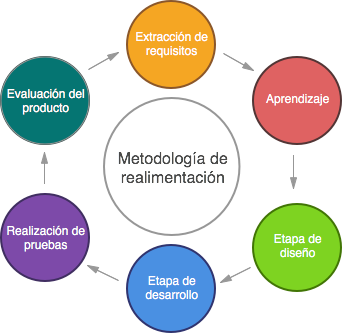
\includegraphics[scale=0.65]{fbackM.png}
\caption{Esquema metodolog�a de realimentaci�n}
\label{fig:metodologia}
\end{figure}


\subsection{Plan de trabajo}
El c�digo fuente de este TFG est� disponible en un repositorio p�blico en GitHub \cite{bazGitRepo} y se ha ido documentando en la Wiki \cite{bazWikiProyect} del mismo. La documentaci�n incluye manuales de uso de los m�dulos principales desarrollados, dise�o de los objetos en la base de datos y un historial descriptivo de las reuniones realizadas con el tutor. La comunicaci�n con el tutor se ha realizado mediante la plataforma Slack y a trav�s de PivotalTracker se han ido estableciendo y completando las diferentes tareas de cada fase del desarrollo del proyecto.
\paragraph{}
El plan de trabajo se ha desarrollado en las siguientes fases:  
\begin{itemize}
\item \textbf{Fase1 - Consolidaci�n, b�squeda y aprendizaje}: esta fase corresponde al proceso de extracci�n de requisitos iniciales y consolidaci�n del concepto de la aplicaci�n, a la b�squeda de herramientas necesarias y al aprendizaje de dichas herramientas (MeteorJS, Javascript, HTML5, CSS3, SASS, WebRTC y RTCRecorder, APIs Soundcloud, AceEditor, IronRouter y dem�s paquetes). 
\item \textbf{Fase 2 - Prototipado:} esta fase ha sido la que m�s tiempo ha requerido y en la que se ha empleado la metodolog�a iterativa descrita anteriormente. En cada iteraci�n se ha enunciado y desarrollado un prototipo cuyo resultado ha servido de base al siguiente. Cada fase ha llevado consigo la realizaci�n de las siguientes tareas:
\begin{enumerate}
	\item Extracci�n de requisitos
	\item Extracci�n de entidades
	\item Dise�o de la base de datos
	\item Dise�o front-end e Interfaces de usuario
	\item Desarrollo de Interfaces
	\item Pruebas y evaluaci�n
\end{enumerate}
\item \textbf{Fase 3 - Final:} una vez implementado el prototipo final se ha procedido a la fase final del proyecto que corresponde a la mejora global y su despliegue. El despliegue implica tambi�n la introducci�n de licencias para preservar los derechos de autor y convertir el c�digo en c�digo libre.
\end{itemize}

\paragraph{}
En el siguiente cap�tulo se describe detalladamente el dise�o y desarrollo de cada los prototipos m�s relevantes que se han implementado a lo largo del proyecto.







\chapter{Dise�o y desarrollo de la aplicaci�n}
\section{Tipo de Arquitectura}
\paragraph{}
El modelo de arquitectura m�s habitual es el \textbf{MVC} (Modelo Vista Controlador) (figura \ref{fig:mvcpattern}). El modelo corresponder�a con la arquitectura de base de datos y el dise�o de la misma, la vista son las interfaces o plantillas que se muestran al usuario y el controlador es el encargado de dotar a la aplicaci�n de l�gica y funcionalidad. Existen otros tipos de arquitectura tales como \textbf{MVVM} (figura \ref{fig:mvvmpattern}), donde el controlador del patr�n MVC se sustituye por VM o \emph{ViewModel} que establece que cada vista posee l�gica y un sistema de \emph{data-binding} entre plantillas.

\begin{figure}[htbp]
    \centering
    \subfigure[Patr�n de arquitectura MVC]{
   	 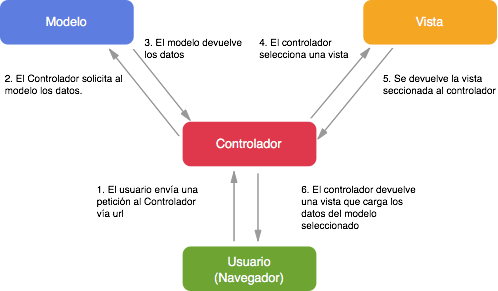
\includegraphics[width=1\textwidth]{mvc.png}
    	\label{fig:mvcpattern}
    }
    \subfigure[Patr�n de arquitectura MVVM]{
    	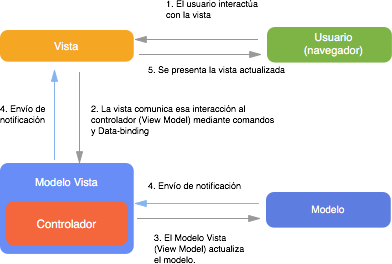
\includegraphics[width=1\textwidth]{mvvm.png}
	 \label{fig:mvvmpattern}
    }
    \caption{Patrones de arquitectura}
    \label{fig:patterns}
\end{figure}

\paragraph{}
La elecci�n del patr�n de arquitectura a usar es importante puesto que esa decisi�n nos limitar� a la hora de usar determinadas herramientas.
\paragraph{}

\section{B�squeda de herramientas}
\paragraph{}
Partiendo de los requisitos establecidos que caracterizar�n la aplicaci�n podemos afirmar que necesitamos encontrar herramientas que nos permitan construir una aplicaci�n en tiempo real, realizar grabaciones de audio, una interfaz con UX (User eXperience) como par�metro fundamental y que trabaje de manera �ptima.

\subsubsection{Aplicaci�n en tiempo real y prototipado r�pido}
\paragraph{}
Necesitamos alg�n framework o plataforma que trabaje con el concepto de reactividad o que lo simule. Elegimos MeteorJS por su flexibilidad, su asombroso concepto de reactividad y por su patr�n de trabajo que engloba el desarrollo del cliente y del servidor. Debido a esta elecci�n utilizaremos MongoDB como tecnolog�a de base de datos y MVVM como patr�n de arquitectura de la aplicaci�n.
\paragraph{}
Para el enrutamiento es precisa otra herramienta que nos proporcione la funcionalidad de especificar a qu� recurso pertenece una plantilla y que datos asociamos a ella. Para ello existen varios paquetes para Meteor que realizan este proceso como IronRouter o FlowRouter. Ambos igual de v�lidos pero para este proyecto se ha optado por IronRouter, ya que dispone de mayor documentaci�n.
\paragraph{}
Para el concepto de publicaciones y subscripciones de Meteor usaremos publishComposite, un paquete que permite realizar publicaciones compuestas (varias colecciones con relaci�n de dependencia reactiva) y que siguen manteniendo el principio de reactividad y optimizando nuestro sistema de subscripciones. Sin este paquete realizar esta labor es m�s compleja. 

\subsubsection{Grabaciones de audio}
\paragraph{}
Existen numerosas formas de grabar audio v�a web y algunas API de sitios como SoundCloud incorporan un grabador de audio directamente. Aunque esta hubiera sido la v�a m�s r�pida, la verdad es que no habr�a sido la m�s flexible, ya que el hacerlo de esta manera requer�a que el uploading se efectuara en SoundCloud. Por este motivo se ha utilizado la tecnolog�a de WebRTC para esta tarea y construido un grabador modular que puede incorporarse f�cilmente a otros proyectos y que adem�s si se desea usar el servicio de hosting de SoundCloud seguir�a siendo factible. 

\subsubsection{Hosting o Almacenamiento}
\paragraph{}
Utilizaremos el servicio de hosting de SoundCloud para almacenar el audio de nuestras grabaciones. No es lo m�s sensato para una aplicaci�n real y comercializable puesto que existen restricciones en lo que corresponde a capacidad, pero para nuestra aplicaci�n es m�s que suficiente. 

\subsubsection{Interfaz con UX como par�metro de dise�o fundamental}
\paragraph{}
Partiendo del requisito de que la aplicaci�n debe ser atractiva al usuario y no s�lo en t�rminos visuales sino en eficacia a la hora de gestionar acciones, en este proyecto nos hemos decantado por el framework front-end Bootstrap para la maquetaci�n y por la tecnolog�a Flexbox para dotar de flexibilidad a las plantillas. Adem�s utilizaremos SASS como preprocesador de CSS con el fin de optimizar nuestra arquitectura de estilos mediante un paquete para Meteor.


\section{Composici�n Inicial y entorno de desarrollo}
\paragraph{}
Una vez realizada la b�squeda de herramientas comenzamos a componer el entorno de nuestra aplicaci�n. Para este proyecto utilizaremos el programa WebStorm de JetBrains. Incorpora herramientas de b�squeda y sustituci�n avanzada, terminal para comandos, integraci�n con sistema de control de versiones Git y plugins que facilitan la labor de desarrollo como elmet.
\subsection{Primeros pasos}
\paragraph{}
Gracias al CLI de Meteor generamos nuestra aplicaci�n mediante el comando: \emph{meteor create $<$AppName$>$}. Esto nos genera una carpeta con tres ficheros: index.html, index.js e index.css. En este momento ya tenemos nuestra aplicaci�n Meteor creada. 
\paragraph{}
Ahora debemos estructurar nuestra aplicaci�n seg�n la jerarqu�a mostrada en la figura \ref{fig:hierarchyFolders} creando los ficheros y carpetas necesarios.

\paragraph{}
Una vez estructurada la aplicaci�n instalamos los paquetes iniciales mediante el comando: \emph{meteor add $<$ PackageName$>$}. La lista de paquetes iniciales es la siguiente: 
\begin{itemize}
\item \textbf{accounts-base:} paquete base para cuentas de usuario.
\item \textbf{accounts-password:} contrase�a como servicio de registro de usuarios.
\item \textbf{fortawesome:fontawesome:} biblioteca de iconos.
\item \textbf{fourseven:scss:} preprocesador Sass para estilos.
\item \textbf{iron:router:} paquete para enrutamiento.
\item \textbf{mizzao:bootstrap-3} maquetaci�n.
\item \textbf{reywood:publish-composite:} publicaciones avanzadas y compuestas.
\end{itemize}

\subsection{Mixins}
\paragraph{}
SASS nos permite crear reglas din�micas de estilos que poder incluir en cualquier clase llamados mixins. Para este proyecto hemos utilizado este concepto para la labor de cross-browsing. Esta labor se basa en la traducci�n de una misma regla a los distintos navegadores Web, ya que cada navegador interpreta algunas reglas de forma distinta. Por lo que estos mixins nos permiten unificar diferentes reglas que se interpretan de manera distinta dependiendo del navegador. Un ejemplo de mixin es el siguiente: 
\begin{lstlisting}[caption=Mixin border-radius, label={mixinEj}]
@mixin border-radius($radius){
	-webkit-border-radius: $radius;  #safari, chrome
	-moz-border-radius: $radius; #mozilla firefox
	-ms-border-radius: $radius; #Internet Explorer
	border-radius: $radius; #new
}
\end{lstlisting}
\paragraph{}
Creamos un fichero con el nombre de \_mixins.scss dentro de la carpeta client al nivel del fichero index.html. El car�cter \_ indica al preprocesador que esta hoja de estilos no la debe procesar. El procesado lo realizar� en el momento que la importemos a otra hoja de estilos e incluyamos alg�n mixin.
Los mixins m�s utilizados en este proyecto ser�n los siguientes: border-radius, flexbox (flex, flex-direction, flex-wrap, etc), opacity, transition, animation y gradient. El archivo est� disponible en el repositorio de GitHub.
\section{Prototipo 1: Registro de usuarios y layout principal}
\paragraph{}
Este es el primer prototipo de la aplicaci�n y se corresponde con el layout principal de la aplicaci�n y con el registro de usuarios. 
\subsection{Layout principal}
\begin{figure}[htbp]
    \centering
    \subfigure[Large layout]{
   	 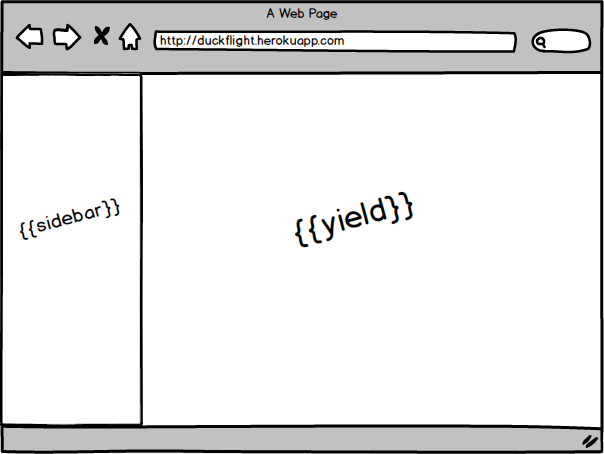
\includegraphics[scale=0.42]{layoutLarge.png}
    	\label{fig:layoutLg}
    }
    \subfigure[Small Layout]{
    	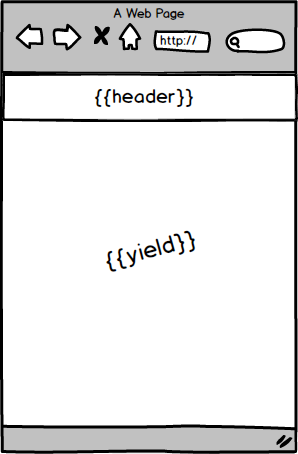
\includegraphics[scale=0.42]{layoutSmall.png}
	 \label{fig:layoutSm}
    }
    \caption{Dise�o de Layout Full-responsive}
    \label{fig:layoutFR}
\end{figure}
Iron Router establece que el dise�o de la aplicaci�n debe realizarse en torno a dos plantillas: \{\{yield\}\} y \{\{layout\}\}. El layout es la plantilla gen�rica y el yield es el contenido. Como puede verse en la figura \ref{fig:layoutFR}, �sta va a ser la estructura gen�rica de nuestra aplicaci�n: 
\begin{itemize}
	\item \textbf{Layout: } estar� compuesta por un sidebar, un header y la plantilla yield.
	\item \textbf{Yield:} esta plantilla es din�mica y se podr� asignar una plantilla u otra dependiendo de la ruta en la que nos encontremos.
\end{itemize}
\paragraph{}
Partiendo del requisito de que los usuarios deben estar autenticados para acceder a la funcionalidad de la aplicaci�n es necesario dise�ar el flujo de registro de usuario y situarlo en un recurso o ruta. Debido a esta restricci�n el flujo se situar� en el recurso ra�z (/). Por lo que, dependiendo de si el usuario est� autenticado o no al acceder a esta ruta deber� mostrarse una plantilla u otra. En este caso:
\begin{itemize}
\item Si el usuario est� autenticado el layout estar� compuesto por la plantilla \{\{$<$sidebar\}\},  \{\{$<$header\}\} y la plantilla \{\{$<$yield\}\} que corresponder� a la plantilla \{\{$<$startPage\}\}.
\item  Si el usuario no est� autenticado el layout estar� compuesto solamente por la plantilla \{\{$<$yield\}\} que corresponder� a la plantilla \{\{$<$mainPage\}\}.
\end{itemize}
El siguiente c�digo muestra el fichero HTML de la plantilla \{\{layout\}\}:
\begin{lstlisting}[language=HTML]
<template name="layout">
    <div id="main-wrapper">
        {{#if currentUser}}
            {{> sidebar }}
            <div id="page-wrapper">
                {{> header}}
                {{> yield }}
            </div>
       	{{else}}
            {{> yield}}
            {{> loginModal }}
        {{/if}}
    </div>
</template>
\end{lstlisting}
El ayudante (helper) currentUser que proporciona Meteor proporciona una funci�n cuyo valor de retorno es un objeto javascript si el usuario est� autenticado o null si no lo est�. Por lo que gracias a Spacebars y sus flujos de control (\{\{if\}\},\{\{else\}\}\,{\{/if\}\}) podemos realizar este dise�o de forma sencilla.

\subsubsection{Sidebar y header}
\paragraph{}
Uno de los requisitos de la aplicaci�n es que debe ser full-responsive. Esto es que se adapte a cualquier tama�o de pantalla. Por lo que es necesario un dise�o adaptativo para cada pantalla de la aplicaci�n en la que el layout no es excepci�n. Como se muestra en la figura \ref{fig:layoutFR}, la plantilla \{\{$<$sidebar\}\} se ocultar� para pantallas estrechas y aparecer� la plantilla \{\{$<$header\}\}. �sta constar� de una serie de botones que al hacer click en cada uno de ellos har� que se se muestre el sidebar con el contenido correspondiente. El dise�o del header puede verse siguiente figura: 
\begin{figure}[hb]
	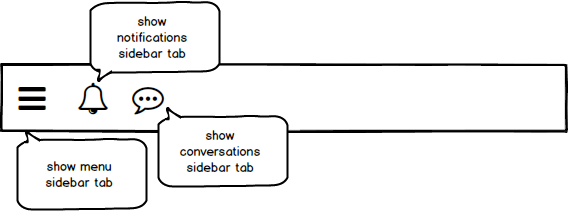
\includegraphics[width=\textwidth]{header}
	\label{fig:header}
	\caption{Dise�o header}
\end{figure}

\paragraph{}
El sidebar est� compuesta por tres espacios diferenciados (figura \ref{fig:sidMenuV1}):
\begin{itemize}
	\item \textbf{Caja Principal:} en ella aparecer� el logo de la aplicaci�n y el nombre que ser�n enlaces al recurso ra�z (/).
	\item \textbf{Contenido:} el contenido del sidebar se organiza mediante un men� de tabs. 
	\item \textbf{Caja de usuario:} en ella aparecer� el avatar y el nombre de usuario que ser�n enlaces al recurso perfil y un bot�n para cerrar sesi�n.
\end{itemize}
\begin{figure}[htpb]
	\centering
	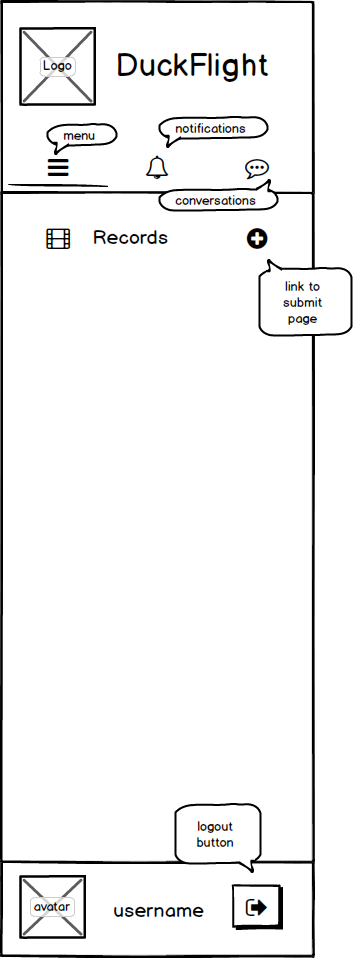
\includegraphics[height=0.72\textheight]{sidebarMenuVersion1}
	\label{fig:sidMenuV1}
	\caption{Dise�o sidebar}
\end{figure}
\subsubsection{Configuraci�n de Iron Router}
\paragraph{}
Iron Router permite establecer una configuraci�n gen�rica para todas las plantillas especificando la plantilla de carga, el layout, plantilla notFound y subscripciones a las colecciones que necesitemos tener accesibles en todo momento. En este prototipo establecemos solamente la plantilla layout.
\paragraph{}
Puesto que acabamos de hablar del primer recurso de la aplicaci�n debemos establecer una ruta para el mismo especificando qu� plantilla ha de mostrarse de la siguiente manera:
\begin{lstlisting}[language=Javascript]
Router.configure({
	layoutTemplate: 'layout'
});

Router.route({'/',
	name: 'mainPage'
});
\end{lstlisting}

\subsection{Registro de usuarios}
\paragraph{}
Para el registro de usuarios creamos una plantilla llamada \{\{>loginModal\}\} que ser� un Modal de bootstrap y que mediante una variable de sesi�n de Meteor mostrar� un formulario para que los usuarios puedan registrarse u otro para que puedan iniciar sesi�n. Esta variable de sesi�n podr�a ser global y podr�a ser utilizada para crear un formulario din�mico que dependiera del valor de dicha sesi�n. Por lo que creamos una plantilla gen�rica para formularios y despu�s incluimos el que correspondiera seg�n el valor de la variable como sigue:

\begin{lstlisting}[language=HTML]
<template name=loginModal>
	<!-- bootstrap modal-->
		{{>formAwesome}}
	<!-- end bootstrap modal-->
</template>
<template name='formAwesome'>
	{{Template.dynamic template=formTemplate}}
</template>

<template name='signInForm'>
	<button></button>
</template>
<template name='signUpForm'>
	<button></button>
</template>
\end{lstlisting}

\begin{lstlisting}[language=Javascript]
//Cuando el modal se renderiza en el DOM, se establece el valor por defecto
//que es que se muestre el formulario para iniciar sesi�n.
Template.loginModal.rendered = function(){
	Session.set('formTemplate','signInForm');
};
Template.formAwesome.helpers({
	//El helper template de la plantilla Template.dynamic hace que dicha 
	//plantilla se sustituya por la indicada en dicho helper
	formTemplate: function(){return Session.get('formTemplate')}
});
Template.signInForm.events({
	//cambiamos al formulario de registro.
	'click button': function(){Session.set('formTemplate','signUpForm')}
});

Template.signUpForm.events({
	//cambiamos al formulario de inicio de sesi�n.
	'click button': function(){Session.set('formTemplate','signInForm')}
});
\end{lstlisting}


\subsubsection{Formulario de inicio de sesi�n}
Atendiendo a los requisitos los usuarios para iniciar sesi�n deber�n rellenar un formulario con dos campos (figura \ref{fig:signIn}):
\begin{itemize}
	\item \textbf{usuario}: nombre de usuario o email.
	\item \textbf{contrase�a}: contrase�a del usuario.
\end{itemize}
El inicio de sesi�n en Meteor se realiza mediante una llamada desde el cliente a la funci�n loginWithPassword proporcionada por el paquete accounts-password pasando como argumento el nombre de usuario o email y la contrase�a.
\subsubsection{Formulario de registro}
Atendiendo a los requisitos los usuarios para registrarse deber�n suministrar un nombre de usuario, una contrase�a y opcionalmente un email (figura \ref{fig:signUp}). El email servir� para la verificaci�n del usuario y para acciones y gestiones que exploraremos m�s adelante. 
\begin{figure}[htbp]
    \centering
    \subfigure[Formulario de inicio de sesi�n]{
   	 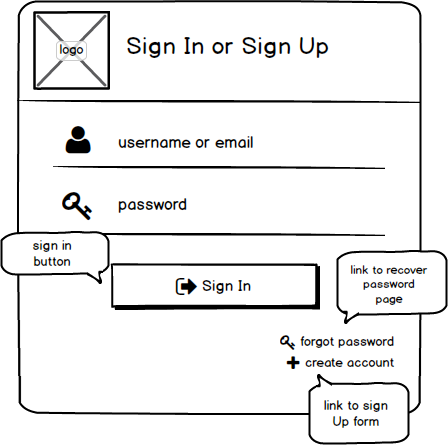
\includegraphics[scale=0.5]{signInForm.png}
    	\label{fig:signIn}
    }
    \subfigure[Formulario de registro]{
    	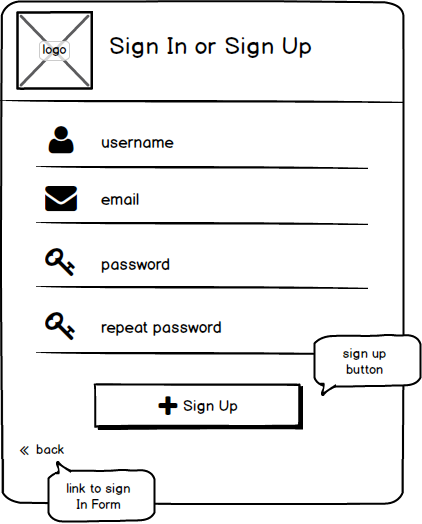
\includegraphics[scale=0.45]{signUpForm.png}
	 \label{fig:signUp}
    }
    \caption{Dise�o formularios de registro}
    \label{fig:signForms}
\end{figure}
El registro de usuarios en meteor se realiza mediante una llamada en el servidor a la funci�n createUser que proporciona accounts-base. Puesto que el evento asociado al click del bot�n se encuentra en el cliente se necesita establecer un method en el servidor que sirva de enlace para el cliente. El cliente llamar� al method y �ste se ejecutar� en el servidor llamando a la funci�n createUser. De forma orientativa se muestra el siguiente c�digo:

\begin{lstlisting}[language=Javascript]
if (Meteor.isClient){
	Template.signUpForm.events({
		'click button': function(e){
			var paramsUser; //extraemos los valores de los campos.
			Meteor.call('signUpMethod',paramsUser,function(err,res){
				if (err) throw new Meteor.error('Error al crear el usuario');
				if (res) console.log(usuario creado con id: res);
			});
		}
	});
};

if(Meteor.isServer){
	Meteor.methods({
		'signUpMethod': function(paramsUser){
			if (userIsValid(paramsUser)){
				return Accounts.createUser(paramsUser,callback)
			}else
				return false;
			}
	})
};
\end{lstlisting}

En el momento que el cliente realiza la llamada con los datos suministrados por el usuario, se deber� verificar que los datos son correctos y que cumplen una serie de reglas. (Validaci�n de nuevo usuario). Una vez verificado se crear� un objeto usuario en la colecci�n disponible en Meteor.users cuya estructura es la mostrada en la figura \ref{userMongo}. En este momento ya tenemos definida la primera entidad de la aplicaci�n (Usuarios).

El resultado de este prototipo puede verse a continuaci�n:
\begin{figure}[htbp]
    \centering
    \subfigure[Formulario de inicio de sesi�n]{
   	 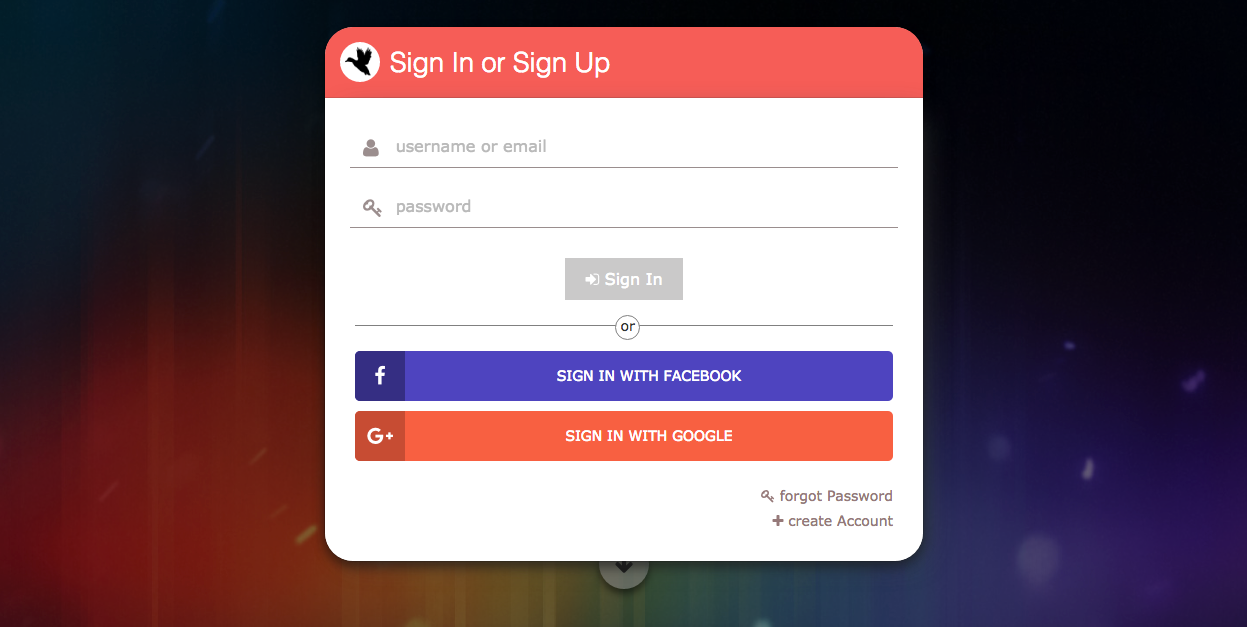
\includegraphics[width=0.7\textwidth]{sign-in-form.png}
    	\label{fig:signInReal}
    }
    \subfigure[Formulario de registro]{
    	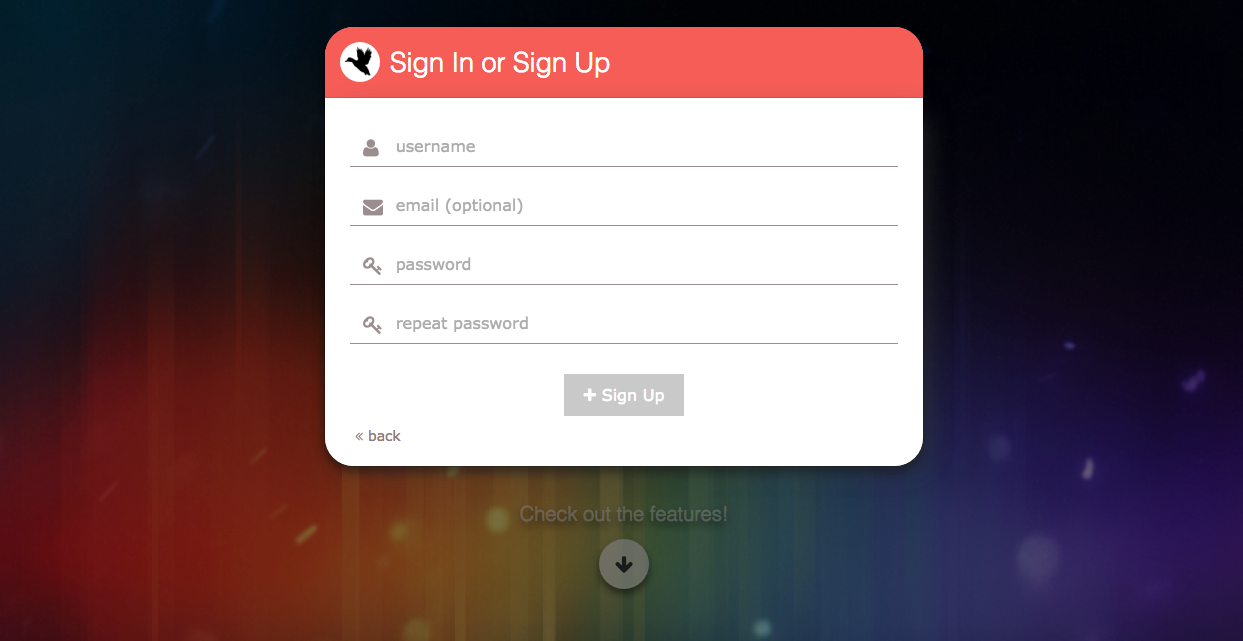
\includegraphics[width=0.7\textwidth]{sign-up-form.png}
	 \label{fig:signUpReal}
    }
    \caption{Formularios de registro en P�gina de inicio}
    \label{fig:signFormsReal}
\end{figure}




\section{Prototipo 2: Grabador y reproductor basados en documentos}
\paragraph{}
Este prototipo engloba el dise�o y desarrollo del grabador, del reproductor y del recurso en el que se muestran las grabaciones realizadas. 
\subsection{Grabador}
\subsubsection{Entidades y colecciones}
\paragraph{}
En este momento surgen dos nuevas entidades de la aplicaci�n que son las grabaciones y los documentos. La relaci�n que existe entre �stas y los usuarios viene determinada por el diagrama mostrado en la figura (TAL). Dicho diagrama impone que cualquier usuario puede crear una grabaci�n y que �sta debe estar formada por uno o m�s documentos. Los documentos no existen independientemente de las grabaciones. Como todas las entidades, �stas se traducen en las colecciones Records y Documents cuyos objetos MongoDB se muestran en \ref{recordMongo} y \ref{documentMongo} respectivamente. Al contrario que la colecci�n Users de Meteor, �stas no se crean por defecto. Por lo que, generamos dos nuevos ficheros javascript: app/lib/collections/records.js y app/lib/collections/documents.js. En cada fichero definimos la colecci�n de la siguiente manera:
\begin{lstlisting}[language=Javascript]
	CollectionName = new Mongo.Collection('collectionName');
	//CollectionName ser� el nombre de la colecci�n accesible en la aplicaci�n.
	//collectionName ser� el nombre de la colecci�n en MongoDB.
\end{lstlisting}
\subsubsection{Routing}

\paragraph{}
Es necesario crear una nueva ruta para el grabador. Esta ruta ser� /records/submit y estar� accesible en todo momento cumpliendo los requisitos gracias a un nuevo dise�o del sidebar que incluye un link a la lista de grabaciones y otro al recurso que acabamos de crear como se muestra en la figura \ref{fig:sidebarV2}.
\paragraph{}
Incluimos una nueva ruta en /app/lib/router.js:
\begin{lstlisting}[language=Javascript]
	Router.route('/records/submit',{
		name: 'recordSubmit'
	});
\end{lstlisting}
\{\{$>$recordSubmit\}\} ser� la plantilla para nuestro recurso.
\subsubsection{Proceso de grabaci�n}
\begin{figure}[h]
    \centering
    \subfigure[Esquema]{
   	 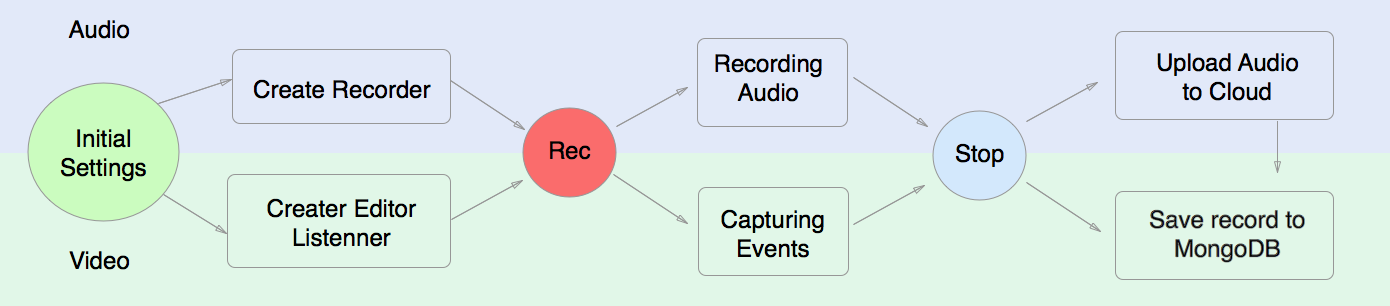
\includegraphics[width=0.8\textwidth]{recordProcess.png}
    	\label{fig:recordProcessSched}
    }
    \subfigure[L�gica]{
    	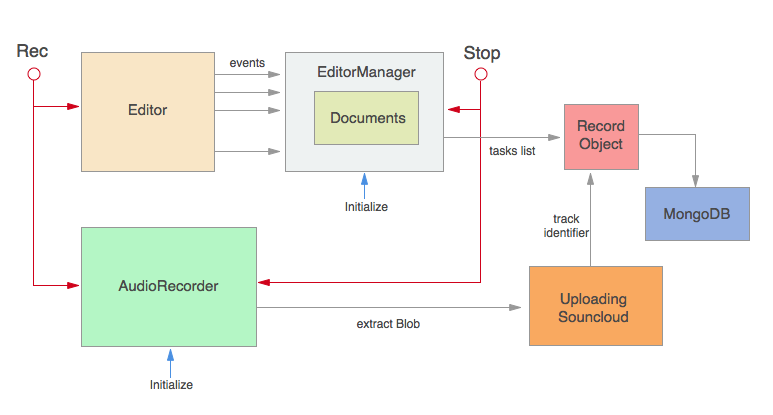
\includegraphics[width=0.8\textwidth]{recordProcessObjects.png}
	 \label{fig:recordProcessLogic}
    }
    \caption{Proceso de grabaci�n}
    \label{fig:recordProcess}
\end{figure}
\paragraph{}
Puesto que cada grabaci�n tendr� dos componentes (audio y video) el proceso se realiza de forma diferente para cada una como se muestra en la figura \ref{fig:recordProcessSched} de forma esquem�tica.
\paragraph{}
Dicho esquema se traduce en la creaci�n de dos objetos javascript: AudioRecorder y EditorManager. Apreciable en la figura \ref{fig:recordProcessLogic}
\begin{itemize}
	\item \textbf{AudioRecorder}: se trata de un constructor que nos permitir� crear un grabador de audio
	\item \textbf{EditorManager}: se trata de un constructor que nos permitir� crear un manejador de documentos, almacenar y actualizarlos de manera din�mica mientras se producen cambios en el editor. 
\end{itemize}
\paragraph{}
La API de RTCRecorder nos proporciona un grabador proporcion�ndole como parametros un el Stream del usuario y una serie de configuraciones. Para conseguir el Stream utilizamos el m�dulo navigator del navegador:

\begin{lstlisting}[language=Javascript]
	navigator.getUserMedia  = navigator.getUserMedia || 
						 navigator.webkitGetUserMedia || 
						 navigator.mozGetUserMedia || 
						 navigator.msGetUserMedia;
	var audioConstraints = {audio: true, video: false};
	navigator.getUserMedia(audioConstraints,function(stream){
		var settings = {}
		var recorder = window.RecordRTC(stream,settings);
		recorder.startRecording();
	},function(error){
		throw new Meteor.error(error.reason);
	});
\end{lstlisting}
El c�digo anterior se encuentra dentro de un m�todo (startRecording) del constructor AudioRecorder y la variable recorder se encuentra accesible por todos los m�todos del mismo por lo que tenemos accesible el grabador proporcionado por RTCRecorder. 
\paragraph{}El proceso de grabaci�n sobre el editor se basa en generar una lista de acciones indexadas por marcas de tiempo. Dichas marcas de tiempo corresponder�n al instante en el que se produce un cambio en el editor y dicho cambio se traducir� en una acci�n (m�todo proporcionado por la API de AceEditor) para que en ese instante durante el proceso de reproducci�n se ejecute dicha acci�n simulando el cambio que se haya producido durante la grabaci�n.
\paragraph{}
Para lo anterior es necesario capturar los cambios del editor, a trav�s de la API de AceEditor, y extraer el instante correspondiente. En el momento que comienza la grabaci�n se ejecuta un callback pasado por par�metro que sirve para arrancar el reloj de la grabaci�n. Dicho reloj ser� accesible dentro de la plantilla \{\{$>$recordSubmit\}\}. Por lo que la sincronizaci�n con los cambios en el editor ser� perfecta.
\paragraph{}
El siguiente c�digo sirve de ejemplo para ilustrar la captura de eventos: 
\begin{lstlisting}[language=Javascript]
var editor = ace.editor('#id');
editor.getSession().on('change', function(e) {
     switch (e.action) {
     	case "remove":
         	var rmRange = {start: e.start, end: e.end};
          docsManagerRecorder.insertFunctions([{
                time: new Date() - date,
                arg: rmRange,
                toDo: 'editor.getSession().getDocument().remove(arg);'
           }]);
           break;
       }
});
\end{lstlisting}
\paragraph{}
Como puede verse en el c�digo anterior docsManagerRecorder es nuestro objeto construido mediante EditorManager y mediante su m�todo insertFunctions generamos nuevas acciones que se simular�n durante la reproducci�n en el instante almacenado en su atributo time.

\paragraph{}
Puesto que una grabaci�n debe estar formada por uno o m�s documentos, durante la grabaci�n puede producirse la creaci�n de nuevos documentos y del cambio de uno a otro sobre el editor. Estos cambios deben ser visibles durante la reproducci�n por lo tanto deben ser capturados. La captura se realiza mediante los eventos que se produzcan en la plantilla correspondiente al crearse un nuevo documento o visualizar otro distinto al actual. En el momento que alguno de estos eventos se produzca se generar� una nueva acci�n que insertar en la lista de acciones mediante el m�todo insertFunctions. 
\paragraph{}
Los eventos posibles que se traducen en acciones son los siguientes: 
\begin{itemize}
	\item Borrar: se borra contenido.
	\item Insertar: se inserta contenido.
	\item Selecci�n: cambia la selecci�n del cursor.
	\item Cursor: cambia la posici�n del cursor.
	\item Scroll: cambia la altura del scroll.
	\item Creaci�n documento: el usuario crea un nuevo documento.
	\item Cambio de documento: el usuario selecciona otro documento distinto al actual para su visualizaci�n.
\end{itemize}

\subsubsection{Almacenamiento}
Como podemos observar en la figura \ref{fig:recordProcess}, una vez termina la grabaci�n se deben proporcionar herramientas para su almacenamiento persistente. El almacenamiento de dicha grabaci�n se realizar� por separado seg�n sus componentes. Un objeto record compuesto por informaci�n sobre la grabaci�n y la lista de acciones (\ref{recordMongo}) se almacenar� en la colecci�n Records de MongoDB y el archivo de audio en SoundCloud. 
\paragraph{}
Para utilizar la API de SoundCloud es necesaria la instalaci�n de un nuevo paquete: monbro:soundcloud-nodejs-api-wrapper  . Este paquete es un wrapper (envoltorio) del SDK (Software Development Kit) de SoundCloud que permite realizar llamadas REST a la API desde el lado del servidor gracias al objeto SoundCloud que nos proporciona de manera global. 
\paragraph{}
Para inicializar dicho objeto necesitaremos un usuario en SoundCloud y crear una aplicaci�n en su espacio para desarrolladores. Dicha aplicaci�n nos proporcionar� una serie de credenciales que nos permitir�n comunicarnos con la API: identificador de la aplicaci�n, clave secreta de la aplicaci�n. Al crearla necesitaremos proporcionarle una url de redirecci�n para la autenticaci�n mediante el protocolo OAuth. 
\paragraph{}
Usando solamente el SDK en el cliente, a la hora de conectar con la API, comenzar�a un proceso de autenticaci�n que mostrar�a un popup que exige interacci�n con el usuario. Dicho proceso no es transparente al usuario y eso es algo que hemos querido arreglar. La soluci�n es incorporar como par�metro de incializaci�n del SDK un token OAuth (el devuelto tras el proceso de autenticaci�n). El problema est� en que dicho token tiene una fecha de expiraci�n y el SDK para Javascript no proporciona herramientas para refrescar el token ya que no tiene m�todo para realizar esa petici�n REST en cuesti�n. Pero el paquete mencionado anteriormente s� tiene esa funcionalidad, y es que cada vez que llamamos a su m�todo .getClient(), nos devuelve un cliente con un token completamente nuevo. 
\paragraph{}
Por este motivo creamos el fichero /app/server/soundcloud.js en el que inicializar el objeto SoundCloud y crear el method .getClientSC al que podemos llamar desde el cliente y que nos devuelve los par�metros necesarios para incializar el SDK del cliente de forma que se conecte a la API de SoundCloud de forma transparente al usuario.
\paragraph{}
El siguiente c�digo ilustra este proceso: 
\begin{lstlisting}[language=Javascript]
if (Meteor.isServer()){
	Soudcloud.setConfig({
		client_id: CLIENT_ID,
		client_secret: CLIENT_SECRET,
		username: USERNAME,
		password: PASSWORD
	});
	
	Meteor.methods({
		getClientSC: function(){
			var client = Soundcloud.getClient();
			return {
				client_id: CLIENT_ID,
				access_token: client.settings.access_token
			}
		}
	});
}
if (Meteor.isClient()){
	$.getScript("https://cdn.WebRTC-Experiment.com/RecordRTC.js",function(){
		Meteor.call('getClientSC',function(err,res){
			if (err) throw new Meteor.error(err.reason);
			if (res){
				SC.initialize({
					client_id: res.client_id,
					oauth_token: res.access_token,
					scope: 'non-expiring'
				});
			}
		});
	});
}
\end{lstlisting}

\paragraph{}
Las variables CLIENT\_ID Y CLIENT\_SECRET contienen el id de la aplicaci�n que hemos creado en Soundcloud y su clave secreta respectivamente.
\paragraph{}
Una vez que tenemos inicializado el SDK en el cliente podemos realizar la subida del audio de la siguiente manera: 
\begin{lstlisting}[language=Javascript]
var recordMongoObject = {};
SC.connect().then(function(){
	SC.upload({
		file: recorder.getAudio(), //Blob
		title: 'title'
	}).then(function(track){
		recordMongoObject.track = {
			id: track.id,
			link: track.uri
		}
		//llamada al servidor para almacenar el objeto.
	})
})
\end{lstlisting}
\paragraph{} 
En el c�digo anterior se muestra c�mo se crea una referencia al archivo subido mediante su identificador. Una vez tenemos el objeto completado realizamos la llamada al method insertRecord, creado en el archivo /app/lib/collections/records.js para almacenar la grabaci�n en MongoDB.


\subsubsection{Interfaz del grabador}
La interfaz del grabador est� formado por dos espacios: la pantalla en la que se mostrar� una plantilla u otra dependiendo de las acciones a realizar y una caja con botones que determinar�n dichas acciones. Adem�s, como se graban documentos sobre editor, constar� de una pesta�a en la que aparecer� el t�tulo del documento que est� siendo editado y un bot�n para acceder a la lista de documentos como se muestra en la figura \ref{fig:recorderBase}

\paragraph{}
El dise�o del grabador se compone de las siguientes plantillas: 
\begin{itemize}
	\item \textbf{\{\{$<$initial\}\}}: es la que se muestra inicialmente y consta de un bot�n para mostrar la lista de documentos.
	\item \textbf{\{\{$<$documentList\}\}}: se muestra como un panel dentro de la pantalla de la interfaz y contiene un bot�n para mostrar el formulario de creaci�n de documentos y la lista de documentos creados. Al hacer click en cada uno de ellos lo visualizaremos en la pantalla. Cada miniatura de los documentos posee un enlace de edici�n que muestra el formulario de creaci�n con los datos del propio documento.
	\item \textbf{\{\{$<$documentForm\}\}}: es el formulario de edici�n y creaci�n de los documentos. Se deber� introducir un t�tulo, un lenguaje de programaci�n y un tema para el editor (estos dos �ltimos son opcionales).
	\item \textbf{\{\{$<$editor\}\}}: plantilla en la que se muestra el editor con el contenido de los documentos.
	\item \textbf{\{\{$<$actions\}\}}: esta plantilla est� presente a lo largo de todo el proceso de grabaci�n y determina las acciones a realizar seg�n el estado del mismo (grabar, parar, guardar/cancelar).
	\item \textbf{\{\{$<$final\}\}}: al finalizar la grabaci�n se muestra en la pantalla de la interfaz un mensaje.
	\item \textbf{\{\{$<$saveForm\}\}}: es el formulario para guardar nuestra grabaci�n. Se deber� introducir un t�tulo y opcionalmente una descripci�n y una lista de etiquetas mediante un auto-completado de etiquetas que se ha elaborado.
	\item \textbf{\{\{$<$upload\}\}}:  al hacer click en guardar en la plantilla anterior se mostrar� el progreso de subida del audio y cuando termine un mensaje y un enlace a la p�gina de la grabaci�n (reproductor) para reproducir la grabaci�n.
\end{itemize}
\paragraph{}
Tras este an�lisis hemos encontrado una nueva entidad: etiquetas (Tags) por lo que creamos una nueva colecci�n y un nuevo fichero en /app/lib/collections de forma an�loga con las anteriores. Establecemos que una grabaci�n puede tener o no etiquetas y que son globales es decir que la misma etiqueta la pueden tener una o varias grabaciones. Esta relaci�n puede verse en el diagrama (tal). Adem�s para tenerlas accesibles desde el formulario debemos crear una publicaci�n a la que se subscribir� el cliente. Como es la primera, creamos el fichero /app/server/publications.js. Ser� el fichero en el que declararemos todas nuestras publicaciones. La subscripci�n a esta publicaci�n se har� din�micamente puesto que se trata de un auto-completado.
\paragraph{}
El flujo de plantillas se muestra en la figura \ref{fig:grabacionFlujo}
Las plantillas presentes en la figura anterior corresponden a las figuras: \ref{fig:recorderNoDocs}, \ref{fig:recorderDocsList}, \ref{fig:documentForm}, \ref{fig:recorderEditor}, \ref{fig:recorderFinal} y \ref{fig:uploadProcess} disponibles en el ap�ndice \ref{appendix:mockupsApendix}.
\paragraph{}
Una vez desarrollado el grabador este es el resultado:
\begin{figure}[htpb]
	\centering
	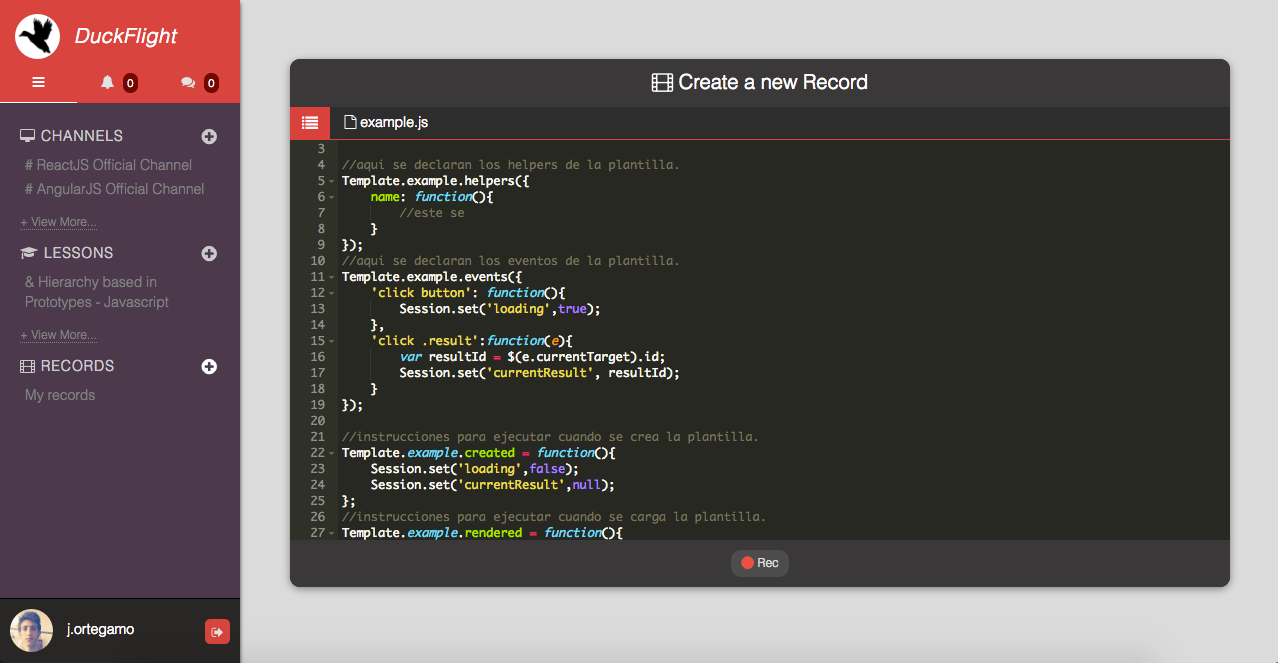
\includegraphics[width=0.75\textwidth]{recorder.png}
	\caption{Grabador}
	\label{fig:recorder}
\end{figure}
\begin{figure}[htpb]
	\centering
	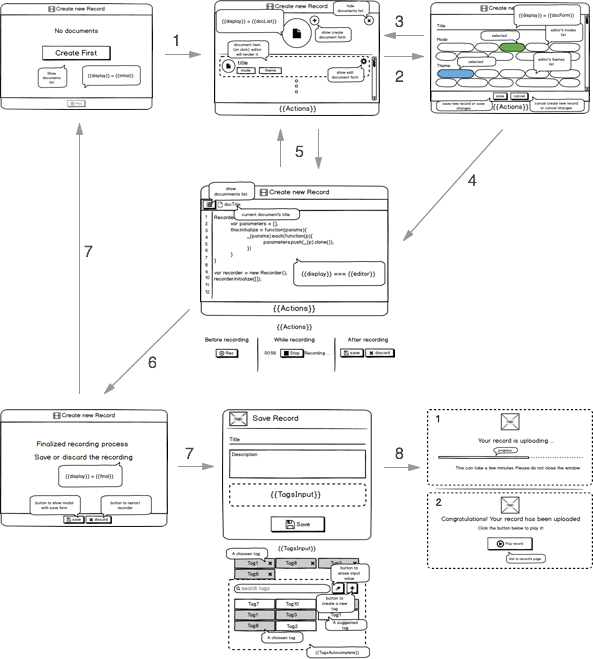
\includegraphics[scale=0.4]{recorderFlow.png}
	\label{fig:grabacionFlujo}
	\caption{Flujo de plantillas del grabador}
\end{figure}
\paragraph{}
\paragraph{}\paragraph{}
\subsection{Reproductor}
\subsubsection{Ruta, publicaciones y subscripciones}
El reproductor es un m�dulo de la p�gina de cada grabaci�n que se establece en una nueva ruta de nuestro proyecto y la primera que establecemos como detalle (detail). La ruta ser� /record/:id donde id corresponder� al identificador del objeto grabaci�n almacenado en MongoDB y estar� configurada en /app/lib/router.js de la misma forma que las anteriores. 
\paragraph{}
La �nica diferencia es que ahora necesitaremos tener accesible el objeto grabaci�n para realizar las acciones oportunas. Esto se consigue creando publicaciones y subscripciones. 

\begin{lstlisting}[language=Javascript]
	// app/server/publications.js
	Meteor.publishComposite('record',function(id){
		//Publicamos el record y los documentos asociados al mismo. 
		var sub = {
			find: function(){
				return Records.find(id)
			},
			children: [{
				find: function(record){
					return Documents.find({record_id: record._id});
				},
				{...}
			}];
		};
		return sub;
	});
\end{lstlisting}
Las subscripciones se realizar�n mediante Iron Router a no ser que sean din�micas. 
\begin{lstlisting}[language=Javascript]
// app/lib/router.js

Router.route('/record/:_id',{
	name: 'record',
	data: function(){
		return Records.findOne(this.params_id);
	},
	waitOn: function(){
		return Meteor.subscribe('record',this.params._id);
	}
});
\end{lstlisting}

De esta manera tendremos accesibles los datos del record y se establecer�n como los datos de la plantilla \{\{$<$record\}\}.

\subsubsection{Proceso de reproducci�n}
Debido a que cada grabaci�n est� compuesta por audio y por v�deo sobre editor, se desarrollan dos procesos paralelos y sincronizados durante la reproducci�n de la misma (figura \ref{fig:playProcessSched}).
\begin{itemize}
	\item \textbf{Audio:} nos conectamos a SoundCloud y realizamos la petici�n del stream del audio correspondiente.
	\item \textbf{V�deo (editor):} a medida que el audio se reproduce, se realiza la simulaci�n de cada evento capturado durante la grabaci�n de forma sincronizada.
\end{itemize}

\begin{figure}[h]
    \centering
    \subfigure[Esquema]{
   	 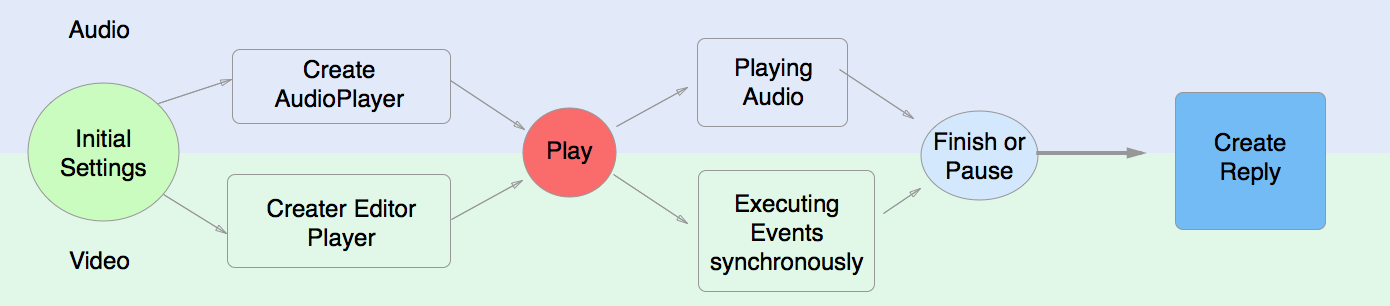
\includegraphics[width=0.8\textwidth]{playProcess.png}
    	\label{fig:playProcessSched}
    }
    \subfigure[L�gica]{
    	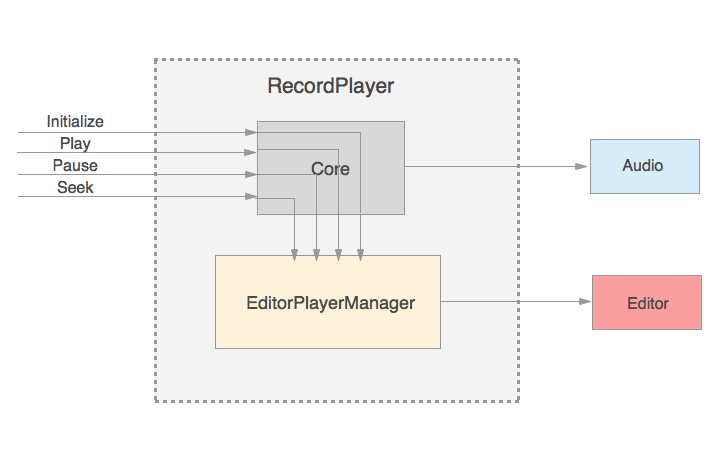
\includegraphics[width=0.8\textwidth]{playProcessObjects.png}
	 \label{fig:playProcessLogic}
    }
    \caption{Proceso de reproducci�n}
    \label{fig:playProcess}
\end{figure}

\paragraph{}
Al igual que durante la grabaci�n, la labor de reproducci�n de cada una de las componentes recaer� en un objeto Javascript: RecordPlayer (audio) y EditorPlayerManager (editor) en los ficheros /app/client/lib/recordPlayer.js y /app/client/lib/editorPlayerManager.js respectivamente (figura \ref{fig:playProcessLogic}).
\begin{itemize}
	\item \textbf{RecordPlayer:} se encarga de ofrecer una interfaz l�gica a partir del stream del audio proporcionado en su inicializaci�n. Dicha interfaz recoge los m�todos necesarios para la reproducci�n (.play(), .pause(), .seek(), .setVolume(), .ended()) y otros propios (.updateCover(), .getState(), .destroy()).
	\item \textbf{EditorPlayerManager:} se encarga de clasificar la lista de acciones capturadas y realizar su simulaci�n. Adem�s se encarga de mantener la integridad de los documentos de la grabaci�n durante el proceso. Este objeto posee los m�todos .getDocs(), .getDocActual(), .update() y .seek().
\end{itemize}
 

\subsubsection{Sincronizaci�n entre audio y editor}

Al inicializar el objeto RecordPlayer toma como argumento un objeto EditorPlayerManager ya inicializado con el identificador del editor. El m�todo .play del objeto RecordPlayer inicia una llamada a su funci�n .updatePlayer() mediante un Interval de 20. Esto quiere decir que cada 20 m�lisegundos se ejecutar� esta funci�n que, a su vez, realiza una llamada a la funci�n .update() del objeto EditorPlayerManager pasado como argumento. Por lo que cada 20 m�lisegundos se mostrar�n cambios en el contenido del editor.

\paragraph{}
Al llamar al m�todo .pause() de RecordPlayer se destruir� la programaci�n del objeto Interval, con lo que parar� de inmediato los cambios sobre el editor. 
\paragraph{}
Al saltar entre instantes de la reproducci�n se llamar� al m�todo .seek(). Este m�todo realiza una llamada directa al m�todo .updatePlayer() y por tanto al m�todo .update() de EditorPlayerManager, pasando como par�metro el instante exacto.

\subsubsection{Simulaci�n de eventos sobre editor}
La simulaci�n se realiza en el m�todo .update() del objeto EditorPlayerManager. El objeto posee la lista de acciones completa, la cual no se alterar� en ning�n momento. Al inicializarse se realiza una copia en una variable global del objeto. En el momento que se produce la llamada al m�todo .update() dicha lista se filtra (se escogen las acciones cuyo instante de creaci�n sea menor o igual que el instante actual de la reproducci�n). Despu�s se clasifican estas acciones y se ejecutan en orden. Despu�s se actualiza el valor de la variable donde estaba la copia de las acciones eliminando de esa lista los ya simuladas. 

\begin{lstlisting}[language=Javascript]
EditorPlayerManager = function(){
	var RC, listPending, editor;
	
	this.initialize = function(params){
		RC = params.RC;
		listPending = RC;
		editor = ace.edit(params.editor);
	};
	
	this.update = function(pos){
		//filtramos las acciones a ejecutar
		var listToDo = _(listPending).filter(function(action){
			return action.time <= pos;
		});
		
		//ejecutamos las acciones que corresponden.
		_(listToDo).each(function(action){
			switch(action.type){
				//ejecuci�n de las funciones guardadas sobre el editor.
			}
		});
		
		//actualizamos la lista de acciones pedientes.
		listPending = _(listPending).difference(listToDo);
	}
}
\end{lstlisting}

El anterior c�digo ilustra el proceso descrito.

\subsubsection{Interfaz del recurso grabaci�n}
\paragraph{}
Se trata de un recurso de detalle (detail resource) y en este proyecto se ha hecho un dise�o base (figura \ref{fig:detailBase}) para este tipo de recurso basado en tres espacios: 
\begin{itemize}
	\item {Banner: } este ser� el espacio dedicado para la presentaci�n de la informaci�n relativa al objeto correspondiente al recurso.
	\item {NavbarTab: } barra de navegaci�n basada en tabs para elegir qu� contenido, asociado al objeto, visualizar.
	\item {tabContent: } espacio en el que se muestran el contenido escogido.
\end{itemize}
\begin{figure}[h]
	\centering
	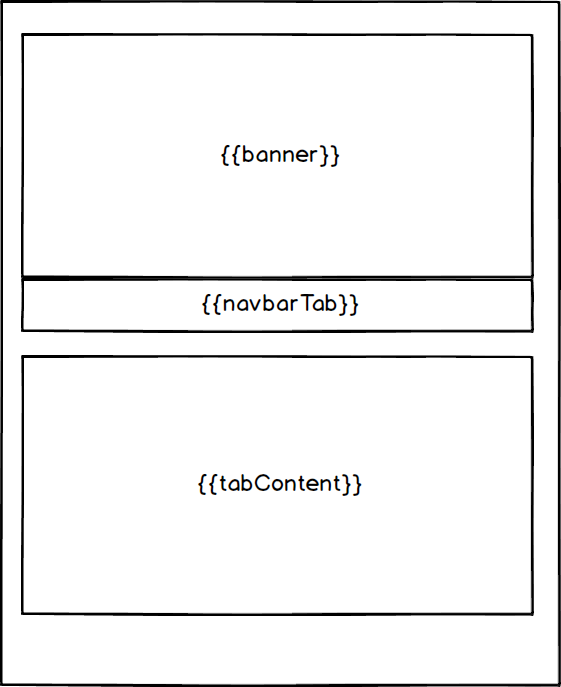
\includegraphics[width=0.5\textwidth]{pageDetailBase.png}
	\caption{Dise�o p�gina de detalle}
	\label{fig:detailBase}
\end{figure}
El banner, en este caso, mostrar� la informaci�n de la grabaci�n (autor, descripci�n, t�tulo, fecha de creaci�n, contadores y lista de etiquetas), un bot�n para votar, la plantilla \{\{$<$player\}\} para el reproductor y la plantilla \{\{$<$actions\}\} como se muestra en el dise�o (figura \ref{fig:recordBanner}).

\begin{figure}[h]
	\centering
	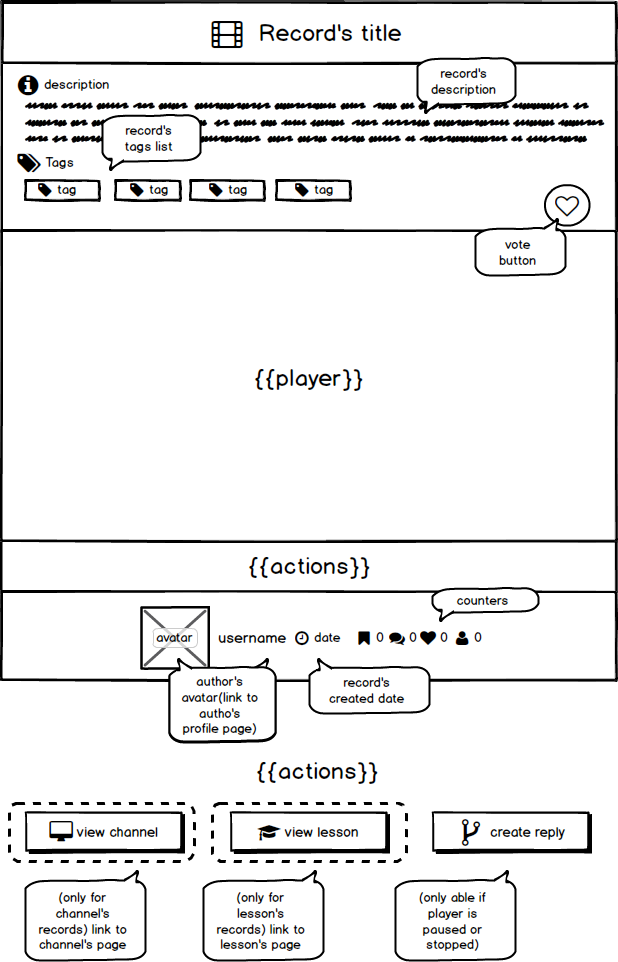
\includegraphics[width=0.6\textwidth, height=10cm]{RecordBanner.png}
	\caption{Dise�o banner para una grabaci�n}
	\label{fig:recordBanner}
\end{figure}

\subsubsection{Interfaz del reproductor}
\begin{figure}[h]
	\centering
	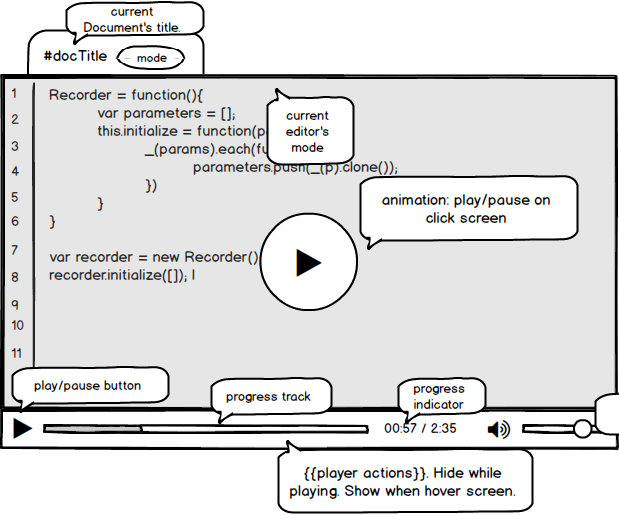
\includegraphics[width=0.7\textwidth]{playerV1}
	\caption{Dise�o interfaz del reproductor}
	\label{fig:playerV1}
\end{figure}
La interfaz del reproductor (figura \ref{fig:playerV1})estar� compuesta por el editor, una capa superpuesta vinculada a los eventos play y pause y la plantilla \{\{$<$playerActions\}\} en la que se muestra el progreso, el timer, un controlador de volumen y los botones play y pause cuando correspondan. Adem�s en la parte superior aparecer� una pesta�a en la que se mostrar� informaci�n sobre el documento actual (t�tulo y lenguaje).
\subsubsection{Streamming}
La plantilla \{\{$<$player\}\} se instancia mediante un helper de la plantilla \{\{$<$record\}\} cuyo valor es un objeto Javascript con los datos necesarios para construir e inicializar los objetos RecordPlayer y EditorPlayerManager y el identificador del audio almacenado en SoundCloud. 
\paragraph{}
Como se muestra a continuaci�n, en el m�todo .rendered() es necesaria la conexi�n con SoundCloud para realizar la petici�n de un stream de audio que poder suministrar al objeto RecordPlayer creado: 
\begin{lstlisting}[language=Javascript]
// app/client/modules/record_modules/record/player.js

Template.player.rendered = function(){
	var self = this.
	Meteor.call('getClientSC',function(err,res){
		if (res){
			SC.initialize ({
				client_id: res.client_id,
				auth_token: res.auth_token,
				scope: 'non-expiring'
			});
			SC.connect().then(function(){
				SC.stream('tracks/' + self.track_id)
					.then(function(s){
						this.recordPlayer.initialize(s,
							this.editorPlayerManager, ...);
					});
			});
		}
	});
}
\end{lstlisting}
\paragraph{}
El resultado final del reproductor puede verse en la siguiente figura: 
\begin{figure}[h]
	\centering
	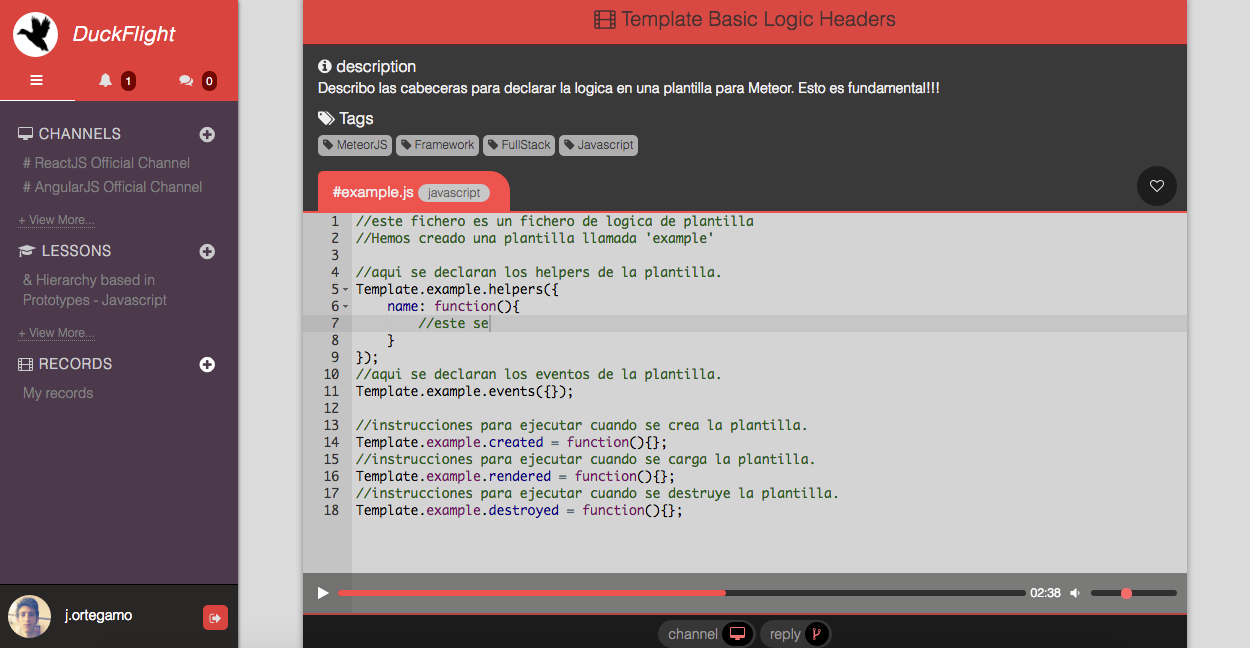
\includegraphics[width=0.8\textwidth]{record-player.png}
	\caption{Reproductor}
	\label{fig:recordPlayerPage}
\end{figure}
\subsection{Lista de grabaciones}
\subsubsection{Ruta, publicaciones y subscripciones}
La lista de grabaciones se mostrar� en una nueva p�gina o recurso de la aplicaci�n. Dicho recurso corresponde a la ruta /records y a la plantilla \{\{$<$records\}\}. Como en cada nueva ruta es necesario integrarla en /app/lib/router.js y, en este caso, crear las publicaciones y subscripciones necesarias.
\begin{lstlisting}[language=Javascript]
// app/server/publications.js

Meteor.publishComposite('records',function(){
	var sub = {
		find: function(){
			return Records.find({},{fields: {RC:0, track: 0, tags: 0}});
		},
		children: [{
			find: function(record){
				return Meteor.users.find(record.author,
						{fields: {username: 1, avatar: 1}});
			}
		}]
	}
});

// app/lib/router.js

Router.route('/records',{
	name: 'records',
	waitOn: function(){
		return Meteor.subscribe('records');
	}
});
\end{lstlisting}
\paragraph{}
De esta manera nos subscribimos a las grabaciones y a los usuarios que las han creado. Filtramos los campos innecesarios para agilizar el proceso de renderizado.
\subsubsection{Interfaz}
La interfaz es muy sencilla (figura \ref{fig:recordsPage}). Est� formada por dos espacios:
\begin{itemize}
	\item \textbf{logo:}  en este espacio se muestra el logo, el t�tulo de la lista y un enlace al recurso creaci�n correspondiente.
	\item \textbf{\{\{$<$recordsTabContent\}\}:} este espacio ser� gen�rico para la aplicaci�n y es que en cualquier parte de la aplicaci�n que se quieran listar grabaciones se utilizar� esta plantilla. Est� formada por:
	\begin{itemize}
		\item \textbf{\{\{$<$contentNavbar\}\}:} en ella aparecen una serie de filtros (recientes, populares), opciones de visualizaci�n y un tab para iniciar el buscador.
		\item \textbf{\{\{$<$content\}\}:} en esta plantilla se listar�n las grabaciones mediante miniaturas (figura \ref{fig:miniaturesRecord}) seg�n el modo de visualizaci�n y aparecer� un bot�n para cargar m�s �tems.
	\end{itemize}
\end{itemize}

Tras el desarrollo de la interfaz el resultado se muestra en la siguiente figura:
\begin{figure}[h]
	\centering
	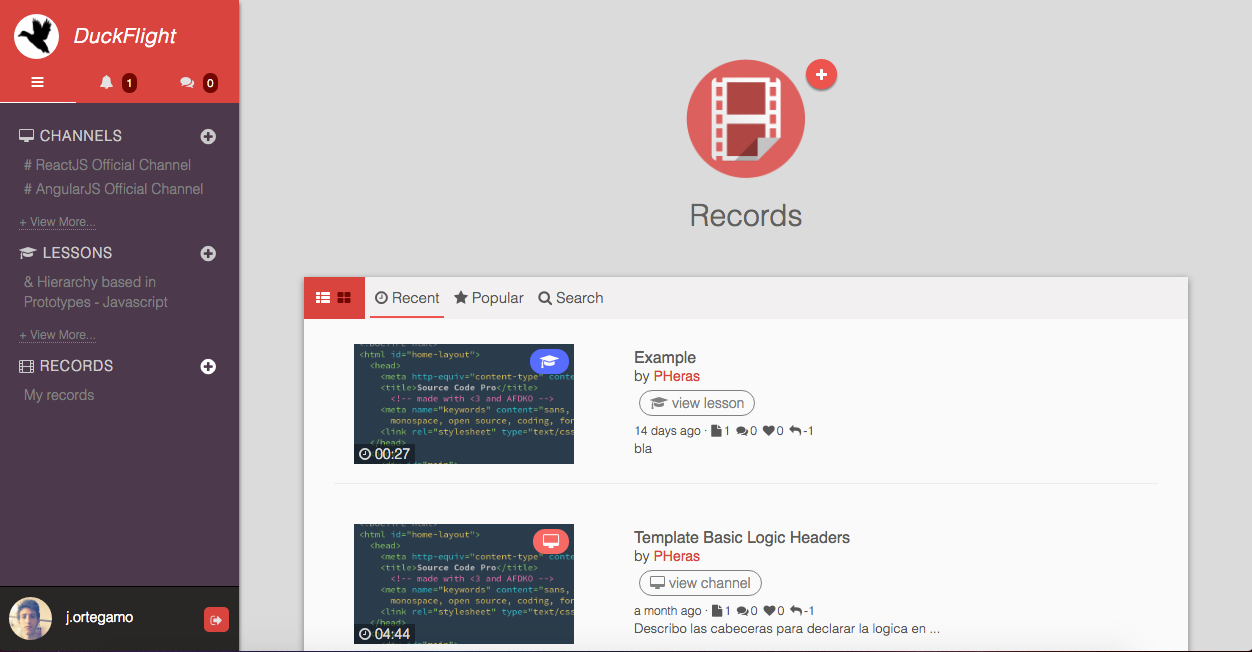
\includegraphics[width=0.8\textwidth]{records.png}
	\caption{Lista de grabaciones}
	\label{fig:records}
\end{figure}
\paragraph{}
\paragraph{}
\section{Prototipo 3: Respuestas a grabaciones}
En este prototipo actualizamos la l�gica del grabador y a�adimos nuevas acciones para la p�gina de detalle de grabaci�n.
\subsection{Actualizaci�n del grabador}
Las respuestas a grabaciones se realizan mediante nuevas grabaciones sobre editor seg�n los requisitos de la aplicaci�n. La �nica diferencia es que esta vez el grabador se debe iniciar con los documentos de la grabaci�n a la que queremos responder. Adem�s el contenido de dichos documentos debe corresponder al instante en el que hemos pausado la reproducci�n. 
\paragraph{}
Para todo lo anterior necesitamos inicializar, con el estado de dichos documentos, al objeto que se encarga de manejarlos durante la grabaci�n (EditorManager).  Pero antes necesitamos extraer dicho estado durante la reproducci�n. Para esto el objeto recordPlayer cuenta con el m�todo .getState() que devuelve un objeto con el �ltimo instante de reproducci�n y la lista de documentos con su estado actual. Dicho objeto se almacenar� en una variable de sesi�n accesible desde el fichero /app/lib/router.js. 
\paragraph{}
Para inicializar el objeto EditorManager como se ha descrito, necesitamos tener esos documentos accesibles desde los datos de la plantilla \{\{$<$recordSubmit\}\}. De esto se encarga Iron Router. La forma de especificar nuestra intenci�n de realizar una grabaci�n respuesta a Iron Router es mediante una query string (cadena de consulta). En ella se especificar� el identificador de la grabaci�n a la que queremos responder y la clave ser� parent\_id.
\begin{lstlisting}[language=Javascript]
Router.route('/records/submit',{
	...
	data: function(){
		var data = {}
		if (this.params.query){ //es una respuesta
			var playerState = (Session.get(playerState));
			(playerState)? data.playInstantObject = playerState : null;
		}
		return data;
	},
	waitOn: function(){
		if (this.params.query){
			return Meteor.subscribe('recordDocuments'
						this.params.query.parent_id);
		}
	}
});
\end{lstlisting}
\paragraph{}En el c�digo anterior podemos ver c�mo se configuran los datos de la plantilla del grabador y c�mo nos subscribimos a los documentos de la grabaci�n padre.
\paragraph{}
Hay que tener en cuenta que en el momento que abandonemos la p�gina del grabador, la variable de sesi�n deber� ser destruida. Esto supone un problema. Si abandonamos la p�gina del grabador y despu�s volvemos a ella, Iron Router interpreta que queremos hacer una grabaci�n respuesta. Esto se debe a que la query string no desaparece. Por este motivo se ha establecido que si volvemos al grabador se comenzar� con los documentos en el estado final de la grabaci�n padre. Dichos documentos los tenemos accesibles gracias a la publicaci�n correspondiente y a la subscripci�n mediante el m�todo waitOn de la ruta descrita en el c�digo mostrado.
\paragraph{}
Como se muestra en el objeto (\ref{recordMongo}), cuando almacenemos la respuesta en MongoDB debemos incluir dos campos: isReply y parent\_id. 
\subsection{Nuevas acciones}
En la plantilla \{\{$<$actions\}\} de la interfaz de detalle de grabaci�n (figura \ref{fig:recordBanner}) creamos dos botones: uno como enlace al grabador para crear una respuesta (s�lo estar� disponible si la reproducci�n se encuentra pausada o finalizada) y otro como enlace a la grabaci�n padre (s�lo disponible si se trata de una respuesta).
\begin{lstlisting}[language=HTML]
<div id='actions'>
	{{#if isPosibleToReply}}
		<button id='reply-button'>reply</button>
	{{/if}}
	{{#if isReply}}
		<button id='go-to-parent-button'>parent</button>
	{{/if}}
</div>
\end{lstlisting}

\begin{lstlisting}[language=Javascript]
Template.record.events({
	'click button#reply-button': function(){
		Session.set('playerState',this.recordPlayer.getState());
		Router.go('recordSubmit',{},{query: 'parent_id=' + this._id});
	},
	'click button#go-to-parent-button': function(){
		Router.go('record',{_id: this.parent_id});
	}
});
\end{lstlisting}

En el c�digo anterior podemos apreciar la l�gica del proceso descrito anteriormente.
\subsection{Timeline, relacionados y comentarios}
En este prototipo se han generado las secciones de contenido de la p�gina detalle de una grabaci�n mostradas en la figura \ref{fig:detailBase}: \{\{navbarTab\}\}(figura \ref{fig:navbarTabDesign}) y \{\{tabContent\}\}. La plantilla \{\{navbarTab\}\} se ha dise�ado como componente de manera que pueda ser configurada con las tabs que correspondan para cada p�gina de detalle.

\paragraph{}
Para listar las respuestas de una grabaci�n se ha creado un timeline (figura \ref{fig:repliesTab}). Dicho timeline se muestra al seleccionar la tab Replies del \{\{$<$navbar\}\} de la p�gina de la grabaci�n.

\begin{figure}[h]
	\centering
	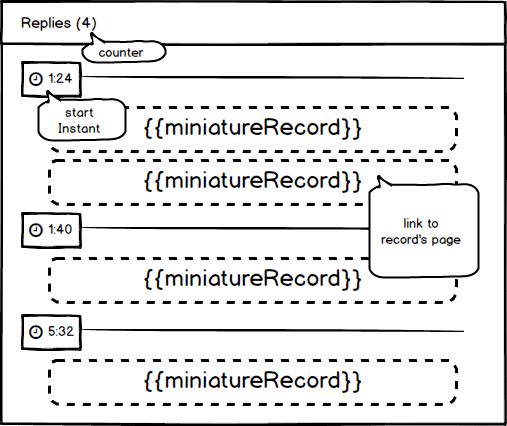
\includegraphics[width=0.7\textwidth]{repliesTab.png}
	\caption{Dise�o de timeline}
	\label{fig:repliesTab}
\end{figure}

\paragraph{}Adem�s se ha a�adido una nueva secci�n de contenidos para mostrar las grabaciones relacionadas con la grabaci�n actual (figura \ref{fig:commentsTab}). Para ello se ha modificado la publicaci�n 'record'. Ahora publicar�, adem�s de la grabaci�n actual, otras que posean etiquetas similares.

\begin{figure}[htpb]
	\centering
	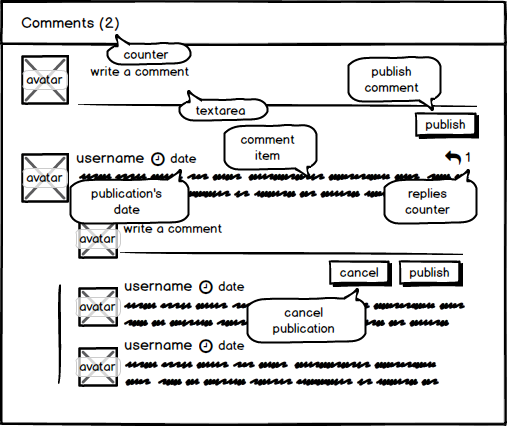
\includegraphics[width=0.7\textwidth]{commentsTab.png}
	\caption{Dise�o del m�dulo de comentarios}
	\label{fig:commentsTab}
\end{figure}

\begin{figure}[htpb]
	\centering
	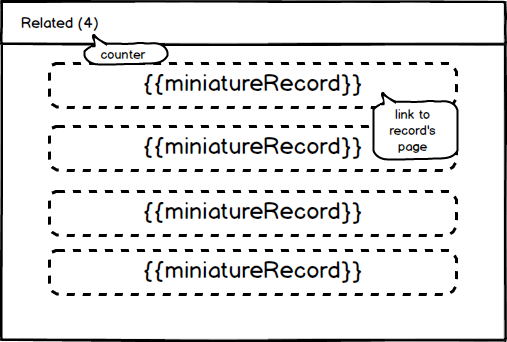
\includegraphics[width=0.7\textwidth]{relatedTab.png}
	\caption{Lista de relacionados}
	\label{fig:relatedTab}
\end{figure}

\paragraph{}Tambi�n se ha creado una nueva secci�n que contiene un espacio para realizar comentarios (figura tal) y con ello surge una nueva entidad. Dicha entidad se traduce en una nueva colecci�n Comentarios cuyo objeto se muestra en \ref{commentMongo} y su relaci�n con las dem�s entidades en la figura \ref{fig:relatedTab}. Esta secci�n esta compuesta por una caja para introducir el texto a publicar y la lista de comentarios. Cada comentario est� compuesto por el avatar del autor, el texto, una lista de las respuestas a ese comentario y la misma caja de texto mencionada anteriormente responder.

\paragraph{}
Se ha dise�ado el espacio para comentarios de manera que sea gen�rico, es decir, que se pueda utilizar para todo tipo de contenidos. Tras la implementaci�n el resultado puede verse en las figuras (tal),(tal) y (tal).




\section{Prototipo 4: Organizaci�n en Canales}
En este prototipo aparece por primera vez el concepto de organizaci�n en canales. La implementaci�n de este concepto deber� cumplir todos los requisitos establecidos en \ref{sec:requisitos} correspondientes. 

\subsection{Concepto, entidades y modificaciones}
Un canal es un espacio p�blico en el que crear grabaciones. Al ser p�blico cualquier usuario puede acceder a sus contenidos de forma inmediata. Tambi�n ofrece la posibilidad de crear comentarios, subscribirse y de votar. 
\paragraph{}
Con esta descripci�n surgen dos nuevas entidades: canales y subscripciones. Dichas entidades se traducen, al igual que las anteriores, en las colecciones Channels y UsersEnrolled respectivamente, cuyos objetos MongoDB son \ref{channelMongo} y \ref{userEnrolledMongo}. Para cada colecci�n se crea un fichero en /app/lib/collections de la misma forma que para las anteriores. La relaci�n entre entidades se muestra en la figura (tal)
\paragraph{}
Puesto que el contenido del canal se constituye en base a las grabaciones, esa relaci�n deber� reflejarse en los objetos de las mismas. Para ello contar�n con el atributo channel\_id las grabaciones pertenecientes a los canales como puede verse en \ref{recordMongo}. Como se describi� en el proceso de grabaci�n, una vez terminada la grabaci�n y completado el proceso de uploading a SoundCloud se proced�a con la creaci�n de un objeto grabaci�n. En esta fase habr� que determinar si la grabaci�n que se ha realizado pertenece a un canal o es independiente. Para ello utilizamos query strings o cadenas de consulta que incluimos en la url del recurso grabador. En este caso la query ser� channel\_id$=$idValue. A modo de ejemplo y siendo el identificador del canal en el que queremos crear una nueva grabaci�n la cadena QwIJOpIsAXzc la url del recurso grabador ser�a /records/submit?channel\_id$=$QwIJOpIsAXzc. Iron Router provee herramientas que permiten realizar esta funci�n de forma sencilla.
\begin{lstlisting}[language=Javascript]
//app/client/modules/channels_module/channel.js
Template.channel.events({
	'click button#create-recording': function(){
		Router.go('recordSubmit',{},{query: 'channel_id=' + this._id});
	}
});

//app/lib/router.js

Router.route('/records/submit',{
	...
	data: function(){
		var data = {};
		(this.params.query.channel_id)? data.channel_id = this.params.query.channel_id : null;
		return data;
	}
})

//app/client/modules/records_module/recordSubmit/recordSubmit.js

SC.upload(audio).then(function(){
	var object = {};
	if (this.data.channel_id){
		object.channel_id = this.data.channel_id;
	}
	Meteor.call('insertRecording',object,function(err,result){});
});
\end{lstlisting}
En el c�digo anterior se muestra un ejemplo de implementaci�n del proceso descrito.
\subsection{Rutas y subscripciones}
Los canales, al ser un contenido m�s en la aplicaci�n deber�n de tener un recurso de creaci�n y su propio recurso. Adem�s contar�n con un recurso de edici�n para cambiar la configuraci�n del mismo.
Estos recursos ser�n: /channels, /channels/submit, /channel/:\_id y /channel/:\_id/edit. 
\paragraph{}
Tanto en el recurso de edici�n como en el propio del canal necesitaremos subscribirnos a los contenidos del canal correspondientes. Por esto creamos una nueva publicaci�n en /app/server/publications.js compuesta por todos los contenidos. A saber: el propio canal, los usuarios subscritos y las grabaciones y comentarios del mismo. Para el recurso de edici�n s�lo es necesario algunos campos del objeto MongoDB del canal. Por lo que creamos una nueva publicaci�n para esta informaci�n. En el recurso /channels necesitaremos subscribirnos a los datos informativos de todos los canales del sitio. Para ello crearemos otra publicaci�n compuesta.
\subsection{Dise�o de interfaces e implementaci�n}
\subsubsection{Creaci�n de un canal}
\begin{figure}[htpb]
	\centering
	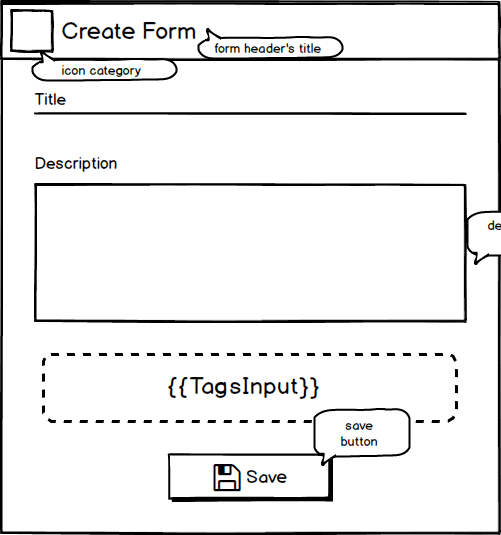
\includegraphics[width=0.7\textwidth]{createChannel.png}
	\caption{Formulario de creaci�n para un canal.}
	\label{fig:createChannel}
\end{figure}
La informaci�n b�sica de un canal estar� formada por un t�tulo, una descripci�n y una lista de etiquetas. La interfaz de creaci�n de un canal deber� permitir la introducci�n de dicha informaci�n (figura \ref{fig:createChannel}). Utilizamos el sistema de formularios din�micos basados en variables de sesi�n que describimos en el prototipo 1 y el complemento de etiquetas que dise�amos en el prototipo 2 para la plantilla \{\{$<$saveForm\}\}. Adem�s creamos un nuevo method en el servidor al que llamaremos desde el cliente para almacenar el objeto canal una vez introducida la informaci�n necesaria.
\begin{lstlisting}[language=Javascript]
//app/lib/collections/channels.js
Meteor.methods({
	insertChannel: function(channelObj){
		return Channels.insert(channelObj);
	}
});

//app/client/modules/channels_module/channelSubmit.js
Template.channelSubmit.events({
	'submit form': function(e,template){
		var obj = {};
		obj.title = template.find('[name=title]').value();
		obj.description = template.find('[name=description]').value();
		obj.tags = Session.get('tagsChosen');
		Meteor.call('insertChannel',obj,function(err,res){
			if (err) throw new Meteor.Error('ERROR insertChannel');
			if (res) console.log('channel inserted with id: ' + res);
 		});
	}
});
\end{lstlisting}
\subsubsection{P�gina de canales}
Este es la p�gina correspondiente al recurso /channels y en ella los usuarios podr�n navegar por la lista de canales del sitio. Su dise�o (figura \ref{fig:channelsPage}) es equivalente al dise�o de la lista de grabaciones y se compone de un logo, un enlace al recurso de creaci�n y un sistema de tabs para realizar filtros y mostrar resultados. Este recurso estar� accesible desde el sidebar como se muestra en la versi�n 3 del mismo (figura \ref{fig:sidebarVersions}).
\subsubsection{P�gina del canal}
Al tratarse de un recurso de detalle, el dise�o base de la interfaz ser� el mostrado en la figura \ref{fig:detailBase}. En el \{\{banner\}\} aparecer� el t�tulo del canal, su descripci�n, la lista de etiquetas, un logo, una imagen de fondo, un enlace al recurso de edici�n y una caja en la que se mostrar� la informaci�n de su creador. Adem�s incorporar� la plantilla \{\{actions\}\} que permitir� subscribirse o cancelar la subscripci�n y votar dicho canal (figura \ref{fig:channelBanner}).
\begin{figure}[htpb]
	\centering
	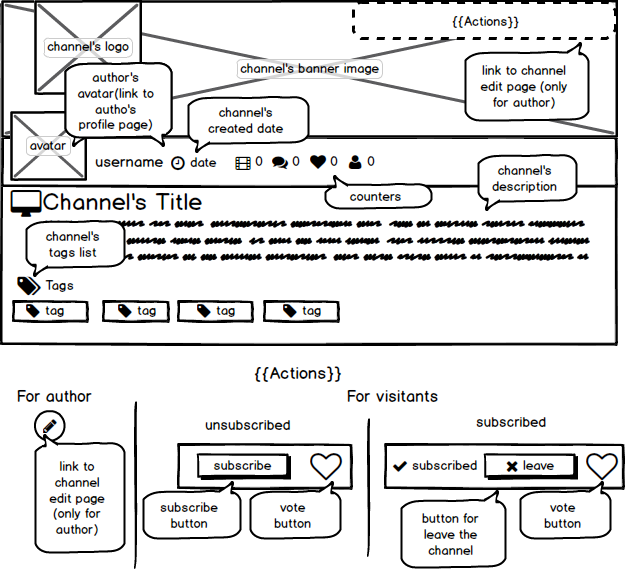
\includegraphics[width=0.7\textwidth]{ChannelBanner.png}
	\caption{Dise�o del banner de un canal}
	\label{fig:channelBanner}
\end{figure}
\paragraph{}
El \{\{navbarTab\}\} contendr� las tabs (figura \ref{fig:navbarTabDesign}): 
\begin{itemize}
	\item \textbf{Recordings:} si se selecciona se mostrar�n en \{\{contentTab\}\} las grabaciones pertenecientes al canal. Dichas grabaciones podr�n ser filtradas por los filtros recientes y populares. Adem�s aparecer� un enlace al recurso de creaci�n para una grabaci�n.
	\item \textbf{Comments:} mostrar� la lista de comentarios realizados.
	\item \textbf{Users:} mostrar� la lista de usuarios subscritos.
\end{itemize} 
\subsubsection{Edici�n de un canal}
En este recurso se podr� editar la descripci�n, el logo, la imagen de fondo y la lista de etiquetas del canal. Utilizamos el sistema de formularios din�micos mediante la inclusi�n de la plantilla \{\{$<$awesomeForm\}\}. Al tratarse del primer recurso de edici�n que nos encontramos en el proyecto, dise�amos una plantilla base (figura \ref{fig:editFormBase}) que podremos reutilizar en cada recurso de este tipo. Dicha plantilla se basa en la incorporaci�n din�mica de complementos o componentes que desarrollaremos para cada tipo de informaci�n y que nos permitir� editarlos. 
\paragraph{}
La entrada y la salida de datos de dicho formulario ser� una variable de sesi�n que configuraremos en la plantilla del recurso de edici�n correspondiente. El valor de dicha variable ser� un objeto con la informaci�n actual del objeto a editar y con una serie de configuraciones que har� que se muestren unos complementos u otros. En este momento se desarrollan los siguientes complementos: 
\begin {itemize}
	\item \textbf{AvatarEdit: } permitir� la edici�n de cualquier tipo de imagen. Las opciones ser�n establecer una por defecto, escoger una desde el disco o introducir una url.
	\item \textbf{DescriptionEdit: } con este complemento editaremos cualquier informaci�n basada en texto mediante un textarea.
	\item \textbf{TagsEdit: } con este complemento editaremos la lista de etiquetas. Adem�s incorpora el sistema b�squeda de etiquetas ya desarrollado.
\end {itemize}
\paragraph{}
El dise�o de estos complementos y el del formulario pueden verse en las figuras \ref{fig:formEditComplements} y \ref{fig:channelEdit} correspondientemente.



\section{Prototipo 5: Organizaci�n en Lecciones}
En este prototipo aparece por primera vez el concepto de organizaci�n en lecciones. La implementaci�n de este concepto deber� cumplir los requisitos establecidos en \ref{sec:requisitos}.

\subsection{Concepto, entidades y modificaciones}
Una lecci�n es un espacio privado en el que crear grabaciones. Esta privaci�n se traduce en que la creaci�n de contenido inmediato para cada lecci�n recae en la figura del usuario creador y que el contenido es privado para los usuarios que no est�n subscritos a la misma. Adem�s la estructuraci�n del contenido de cada lecci�n estar� basada en secciones.
\paragraph{}
Con la anterior descripci�n surgen dos nuevas entidades: lecciones y secciones. Estas entidades se traducen en las colecciones Lessons y Sections cuyos objetos son \ref{lessonMongo} y \ref{sectionMongo} respectivamente. Se crean los ficheros /app/lib/collections/lessons.js y /app/lib/collections/sections.js en los que se declarar�n las colecciones y se implementar�n los methods para gestionar sus modificaciones. Su relaci�n con las dem�s entidades se muestra en la figura (tal).
\paragraph{}
Cada secci�n estar� compuesta de grabaciones. Por lo que dichas grabaciones har�n referencia a la secci�n y a la lecci�n que pertenecen, adem�s de indicar el orden dentro de la secci�n. Cada secci�n poseer� tambi�n un orden dentro de cada lecci�n. Estos par�metros ser�n necesarios a la hora de editar las listas en el recurso de edici�n de la lecci�n. Al igual que para las grabaciones pertenecientes a un canal, informamos al grabador de que se trata de una grabaci�n perteneciente a una lecci�n mediante la url. Esta vez formada por varias query string: lesson\_id, section\_id y order (\ref{recordMongo}). 
\begin{lstlisting}[language=Javascript]
//app/lib/router.js
Router.route('record/submit',{
	...
	data: function(){
		var data = {};
		....
		(this.params.query.lesson_id)? data.lesson_id = this.params.query.lesson_id : null;
		(this.params.query.section_id)? data.section_id = this.params.query.section_id : null;
		(this.params.query.order)? data.order = this.params.query.order : null;
	}
});

//app/client/modules/record_modules/recordSubmit/recordSubmit.js
SC.upload(file).then(function(){
	var obj = {}
	if (this.data.lesson_id){
		obj.lesson_id = this.data.lesson_id;
		obj.section_id = this.data.section_id;
		obj.order = this.data.order;
	}
	Meteor.call('insertRecord',obj,function(err,res){});
});
\end{lstlisting}
\subsection{Rutas y subscripciones}
Los recursos que se establecen para este contenido son: /lessons/submit, /lessons, /lesson/:\_id y /lesson/:\_id/edit (creaci�n, listado, propio y creaci�n).
\paragraph{}
Creamos una publicaci�n compuesta para el recurso detalle, una publicaci�n simple para el recurso de edici�n y otra compuesta para el recurso de listado a las que nos subscribiremos mediante el m�todo .waitOn de cada ruta establecida en /app/lib/router.js para cada recurso.
\subsection{Lista de reproducci�n y opciones}
\begin{figure}[htpb]
	\centering
	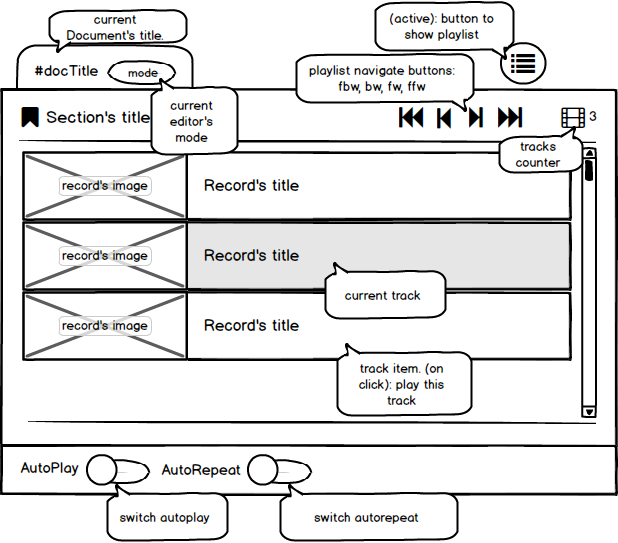
\includegraphics[width=0.7\textwidth]{playlist.png}
	\caption{Dise�o lista de reproducci�n}
	\label{fig:playlist}
\end{figure}
Debido a que el contenido de las lecciones se estructura en secciones que no son m�s que una lista de grabaciones, introducimos el concepto de lista de reproducci�n para el proyecto. Esto es, cuando reproduzcamos una grabaci�n perteneciente a una lecci�n, el reproductor mostrar� la lista de grabaciones de la secci�n a la que pertenece. Adem�s permitir� la navegaci�n por ella y establecer las opciones de reproducci�n y repetici�n autom�tica. 
Estas configuraciones se realizar�n en el objeto del usuario mediante los atributos: auto\_play y auto\_repeat. Las funciones son las siguientes: 
\begin {itemize}
	\item \textbf{Reproducci�n autom�tica: } al terminar la reproducci�n de cada elemento de la lista se comienza con la del siguiente.
	\item \textbf{Repetici�n autom�tica: } convierte la lista de grabaciones en una lista circular. El elemento siguiente del �ltimo es el elemento primero y el elemento anterior al primero es el �ltimo.
\end{itemize}
\paragraph{}
Si se da el caso de que ambas funciones est�n activadas, la reproducci�n de la lista de grabaciones de una secci�n es infinita.
El dise�o de la misma puede verse en la figura \ref {fig:playlist}
\subsection{Dise�o de interfaces e implementaci�n}
\subsubsection{Creaci�n de una lecci�n}
La informaci�n b�sica de una lecci�n est� formada por un titulo, una descripci�n y una lista de tags. Para su implementaci�n utilizamos el sistema de formularios din�micos mediante variables de sesi�n e integramos en la plantilla del formulario (figura \ref{fig:createChannel}) los complementos que permitan la introducci�n de dicha informaci�n (los mismos que para el recurso de creaci�n de un canal).
\subsubsection{P�gina de lecciones}
En esta p�gina los usuarios podr�n explorar las lecciones del sitio. Su dise�o (figura \ref{fig:lessonsPage}) esta formado por un logo, un enlace al recurso de creaci�n para las lecciones y un sistema de tabs. Este sistema de tabs es el mismo que hemos desarrollado para la p�gina de las grabaciones. Este recurso estar� accesible desde el sidebar como se muestra en la versi�n 3 del mismo (figura \ref{fig:sidebarVersions}).
\subsubsection{P�gina de una lecci�n}
\begin {figure}[htpb]
	\centering
	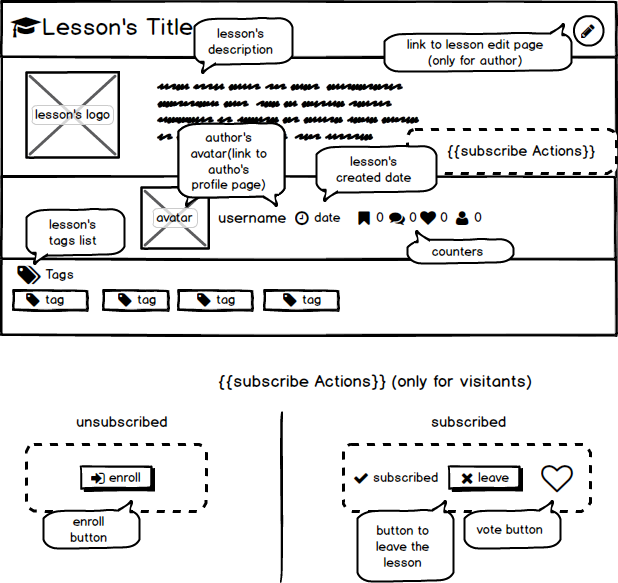
\includegraphics[width=0.7\textwidth]{LessonBanner.png}
	\caption{Dise�o del banner de una lecci�n}
	\label{fig:lessonBanner}
\end{figure}
Al tratarse de un recurso de detalle, tendr� el mismo dise�o base que con los que comparte dicha clasificaci�n (figura \ref{fig:detailBase}). En el \{\{banner\}\} aparecer� el t�tulo de la lecci�n, el logo, la descripci�n, un apartado con la informaci�n sobre el autor y los contadores de la lecci�n, la lista de etiquetas y la plantilla \{\{actions\}\} que permitir� a los usuarios realizar determinadas acciones seg�n su rol: 
\begin{itemize}
	\item \textbf{Autor: } podr� votar y acceder al recurso de edici�n.
	\item \textbf{Visitante: } si est� subscrito podr� votar y cancelar su subscripci�n y, si por el contrario, no lo est�, podr� subscribirse.
\end{itemize}
\paragraph{}
El \{\{navbarTab\}\} contendr� las tabs (figura \ref{fig:navbarTabDesign}):
\begin{itemize}
	\item \textbf{Sections: } si se encuentra seleccionada, en \{\{contentTab\}\} se mostrar� el listado de las secciones y un bot�n para acceder a un modal con el formulario para crear las mismas.
	\item \textbf{Comments: } lista de comentarios de la lecci�n.
	\item \textbf{Users: } lista de usuarios subscritos.
\end{itemize}
\paragraph{}
Cada �tem secci�n estar� formado por una cabecera y por un sistema de tabs implementado mediante un collapsible de Bootstrap. Ciertas acciones sobre estos elementos ser�n accesibles o no dependiendo del rol del usuario bas�ndonos en los requisitos establecidos. Esto se refleja en la figura \ref{fig:sectionsTab}. Cada �tem en su cabecera mostrar� el n�mero de grabaciones, un bot�n para eliminar la secci�n, un bot�n para reproducir los contenidos y un enlace al recurso de creaci�n de las grabaciones (grabador). El sistema de tabs estar� formado por dos pesta�as. En una aparecer� la lista de grabaciones (enlaces al reproductor) y en la otra la lista de grabaciones con botones para editar el orden dentro de la secci�n. Todas las acciones que pretendan crear, modificar o borrar est�n suprimidas para los usuarios con el rol de visitante.
\subsubsection{Edici�n de una lecci�n}
Al tratarse de un recurso de edici�n, utilizamos el dise�o implementado anteriormente. La plantilla \{\{$<$awesomeForm\}\} para cargar el formulario base mostrado en la figura \ref{fig:editFormBase} y a dicho formulario integramos los componentes \ref{fig:formEditComplements} avatarEdit, descriptionEdit, tagsEdit y adem�s creamos uno nuevo para poder editar el orden de las secciones. El dise�o se muestra en la figura \ref{fig:lessonEdit} 

\section{Prototipo 6: P�gina de perfil y Contactos}
En este prototipo se ha dise�ado e implementado la p�gina de perfil del usuario y un espacio para realizar solicitudes de contacto y mostrar esas relaciones entre los distintos usuarios.
\subsection{Perfil}
Se trata de un nuevo m�dulo y recurso cuya ruta ser� /profile/\_id, donde \_id corresponder� al id del usuario en cuesti�n. Se crean nuevas publicaciones y subscripciones y se establece la ruta en /app/lib/router.js.

\subsubsection{Interfaz}
Al tratarse de un recurso de detalle compartir� la misma base que los dem�s (figura \ref{fig:detailBase}). El \{\{banner\}\} estar� formado una cabecera en la que se muestran el avatar del usuario, una imagen de fondo, un bot�n para acceder al recurso de edici�n del perfil y una caja con acciones y un cuerpo en el que aparece el nombre de usuario, la descripci�n y lista de servicios (figura \ref{fig:profileBanner}). 

\begin{figure}[htpb]
	\centering
	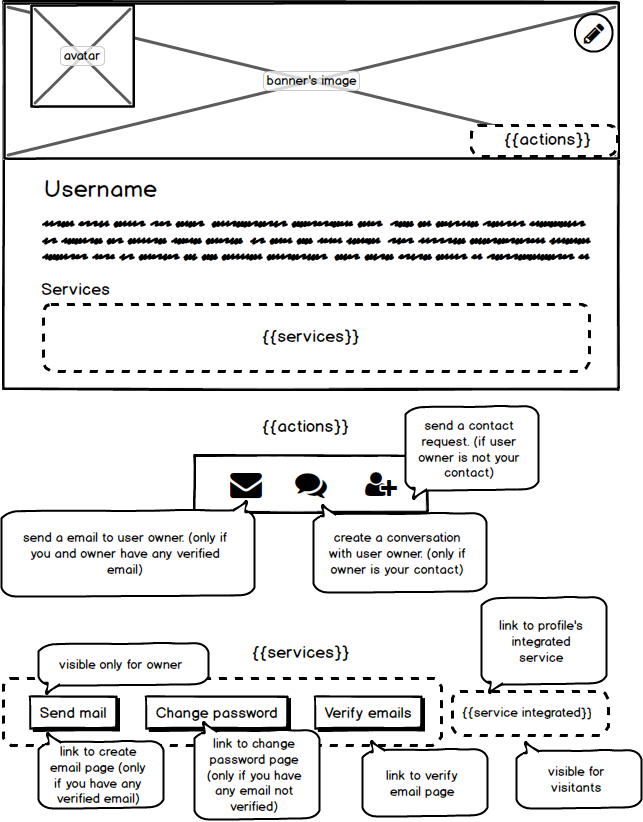
\includegraphics[width=0.9\textwidth]{profileBanner.png}
	\caption{Dise�o banner del perfil}
	\label{fig:profileBanner}
\end{figure}

\subsubsection{Contenidos}
Utilizamos el complemento navbarTab y lo configuramos para que tenga las tabs canales, lecciones, grabaciones, conversaciones y contactos que corresponden a las categor�as de contenido de la aplicaci�n (figura \ref{fig:navbarTabDesign}).
Podemos reutilizar las plantillas  \{\{contentTab\}\} para mostrar las listas de contenido seg�n la categor�a que hemos generado para los recursos /records, /channels y /lessons. S�lo aparecer�n las del usuario en cuesti�n, ya que nos hemos subscrito a sus contenidos. Aunque en este caso no existe la opci�n de iniciar el buscador, sino que se a�aden nuevos filtros (figuras \ref{fig:recordsPage}, \ref{fig:lessonsPage} y \ref{fig:channelsPage} ): 
\begin{itemize}
	\item \textbf{Subscrito: }muestra los canales o lecciones a los que se ha subscrito el usuario seg�n corresponda.
	\item \textbf{Historial: }muestra un total de 10 entradas. Dichas entradas ser�n las 10 �ltimas reproducciones que el usuario haya visualizado y formar�n parte del  \{\{contentTab\}\} para las grabaciones.
\end{itemize}
\paragraph{}
Adem�s se han incluido nuevos enlaces en el sidebar para acceder a los contenidos del perfil de forma directa mediante una query string que establece el contenido a visualizarse al cargar el perfil como puede verse en el dise�o MenuTabV4 del sidebar (figura \ref{fig:sidebarVersions}). Tambi�n se han incluido los enlaces necesarios en todas las cajas de usuario de los recursos detalle y en sus miniaturas.
\subsubsection{Roles}
Al visualizar cualquier p�gina de perfil un usuario puede adoptar uno de estos dos roles: 
\begin{itemize}
	\item \textbf{Propietario:} lo adoptar� el usuario que sea propietario de dicho perfil. Podr� acceder a la lista de servicios y al recurso de edici�n del perfil, adem�s en cada \{\{contentTab\}\} se le mostrar� un enlace al recurso de creaci�n correspondiente. 
	\item \textbf{Visitante:}  lo adoptar� el usuario que no sea propietario de dicho perfil. Podr� acceder a las acciones presentes en la cabecera del banner. S�lo existir� una, de momento: realizar peticiones de contacto.
\end{itemize}
\subsubsection{Edici�n del perfil}
Al igual que para editar las lecciones o los canales se establece un nuevo recurso para editar el perfil cuya ruta es /profile/:\_id/edit. Como en las otras es necesario declararla en /app/lib/router.js crear una nueva plantilla \{\{$<$profileEdit\}\} en /app/client/modules/profile\_modules/profileEdit/profileEdit.html y subscribirse al usuario correspondiente. Al igual que los dem�s recursos de edici�n, �ste mantiene el dise�o base (figura \ref{fig:editFormBase}), es decir, que incorpora la plantilla \{\{$<$awesomeForm\}\} la cual, mediante una variable de sesi�n, carga uno u otro formulario con caracter�sticas comunes. En este caso, el formulario de edici�n din�mico creado en el prototipo 4. Adem�s incorporamos los componentes avatar, banner y description (figuras \ref{fig:profileEdit}, \ref{fig:formEditComplements}). 
\subsection{Contactos}
Al existir usuarios en la aplicaci�n es necesario establecer y denominar las relaciones entre ellos. Dichas relaciones se denominan relaciones de contacto. Con esto surge una nueva entidad (Contactos) que se traduce en una nueva colecci�n Mongo llamada Relations con su fichero correspondiente y cuyo objeto es \ref{relationMongo}


\subsubsection{Peticiones y lista de contactos}
Surge una nueva entidad Peticiones que se traduce en la colecci�n llamada Requests cuyo objeto es \ref{requestsMongo} 
Para el \{\{contentTab\}\} del tab 'contactos' \ del \{\{navbarTab\}\} de la p�gina de perfil se establecen dos nuevas tabs: contactos y peticiones.
\paragraph{}
Para la tab contactos activa se mostrar� la lista de los contactos (figura \ref{fig:contactsTab}). Cada miniatura contar� con el avatar, el nombre de usuario, la fecha desde la que se inici� la relaci�n de contacto, la descripci�n y acciones (s�lo visibles cuando el usuario es el propietario del perfil).

\paragraph{}
Para la tab peticiones activa se mostrar� el espacio para peticiones (figura \ref{fig:requestsTab}). Dicho espacio esta compuesto por: 
\begin{itemize}
	\item Autocompletado: para buscar los usuarios. Cada resultado dispondr� de un bot�n para enviar la petici�n. Este bot�n se sustituir� por iconos de estado si la petici�n ya ha sido realizada. 
	\item Bandeja de entrada: se muestran las peticiones recibidas, su estado y acciones relacionadas con su estado.
	\item Bandeja de salida: se muestran las peticiones enviadas, su estado y acciones relacionadas con su estado.
\end{itemize}

Las acciones dependiendo del estado y de la bandeja en la que se encuentren se muestran en la tabla \ref{tabla:requestsActions}: 

\begin{table}[htb]
\centering
\begin{tabular}{|l|l|l|}
\hline
& \multicolumn{2}{c|}{Acciones} \\
\hline
Estado & Recibidas & Enviadas\\
\hline
Pendiente & Aceptar o Rechazar & X\\ \hline
Aceptada & Ok & Ok\\ \hline
Rechazada & X & Ok o Reenviar \\ \hline
\end{tabular}
\caption{Acciones para las peticiones}
\label{tabla:requestsActions}
\end{table}

El proceso para establecer la relaci�n de contacto es la siguiente: 
\begin{enumerate}
	\item El usuario A env�a una solicitud al usuario B y visualiza esta petici�n como pendiente.
	\item El usuario B visualiza la petici�n como pendiente en su bandeja de entrada y puede aceptarla o rechazarla.
	\item El usuario B acepta la petici�n y la visualiza como aceptada, pulsa Ok. Se crea la relaci�n.
	\item El usuario A visualiza la petici�n como aceptada, pulsa Ok para eliminar la entrada.
\end{enumerate}

\paragraph{}Si el usuario B rechaza la petici�n, el usuario A la visualizar�a como rechazada y podr�a pulsar Ok o reenviarla y comenzar el proceso de nuevo.

\paragraph{}Adem�s de realizar las peticiones mediante este espacio, se habilita para los usuarios que tengan el rol de visitante un bot�n en \{\{actions\}\} como se muestra en la figura (\ref{fig:profileBanner}).

\paragraph{}La implementaci�n de este prototipo tiene como resultado las figuras (tal tal tal en ap�ndices).


\section{Prototipo 7: Conversaciones y alertas}
En este prototipo se ha dise�ado y desarrollado el m�dulo de comunicaciones interno de la aplicaci�n basado en conversaciones o chats. Tambi�n el sistema de alertas y avisos de nuevos mensajes.
\subsection{Conversaciones}
\subsubsection{Entidades, Rutas, subscripciones y publicaciones}
Se trata de otra categor�a de contenidos dentro de la aplicaci�n por lo que tendr� un recurso de creaci�n, de detalle y de edici�n: /conversation/submit, /conversation/:\_id y /conversation/:\_id/edit. El acceso a las conversaciones es privada, es decir, s�lo los miembros pueden visualizarlas. Esto se traduce en que el listado de las mismas est� disponible como contenido dentro del recurso perfil de cada usuario y s�lo ser� visible si el usuario tiene el rol de propietario.
\paragraph{}
Con la aparici�n de esta nueva categor�a surgen las nueva entidades Conversaciones y Mensajes que se traducen en las colecci�nes Conversations (/app/lib/collections/conversations.js) y Messages (/app/lib/collections/messages.js) y cuyos objetos se definen en \ref{conversationMongo} y \ref{messageMongo}. La relaci�n de �stas con las dem�s entidades queda reflejada en la figura (tal).
\paragraph{}
Al igual que para las anteriores categor�as, se han creado las publicaciones necesarias a las que nos subscribiremos mediante Iron Router en las rutas establecidas a los recursos de detalle y de edici�n.
\subsubsection{Roles}
Los roles en las conversaciones ser�n importantes a la hora de ofrecer a los usuarios diferente funcionalidad. Los miembros de una conversaci�n se pueden clasificar seg�n sus roles en:
\begin{itemize}
	\item \textbf{L�der: } tiene acceso a todas las caracter�sticas de la conversaci�n. Podr� expulsar usuarios, cambiar el asunto, a�adir a nuevos miembros como invitados e, incluso, delegar su rol a otro miembro.
	\item \textbf{Invitados: } �stos tendr�n acceso a las mismas funciones que el l�der a excepci�n de expulsar usuarios y de cambiar el asunto.
\end{itemize}
\subsubsection{Creaci�n de una conversaci�n}
Puesto que las conversaciones son privadas, el �nico medio para acceder a su recurso de creaci�n es desde el recurso perfil. Al igual que los anteriores, este recurso utiliza la plantilla \{\{$<$awesomeForm\}\} que mediante la variable de sesi�n 'typeForm' incluir� la plantilla base para un formulario de edici�n. Esta plantilla incorporar� los componentes correspondientes para la introducci�n de la informaci�n necesaria. Estos son una caja de texto para el asunto y dos complementos que se han implementado para la introducci�n de miembros y del primer mensaje (figura tal).

\subsubsection{P�gina de conversaci�n}
Este ser� el primer y �nico recurso de detalle que no compartir� con los dem�s el dise�o base formado por un \{\{banner\}\}, \{\{navbarTab\}\} y \{\{contentTab\}\}. El dise�o corresponder� al mostrado en la figura (tal) que se compone de tres espacios: 
\begin{itemize}
	\item \textbf{Cabecera: } aqu� se mostrar� toda la informaci�n relevante de la conversaci�n (asunto, lista de miembros, contadores), botones para para visualizar el panel de miembros, el panel de opciones y acceder al recurso de edici�n.
	\item \textbf{Cuerpo: } corresponde a la lista de mensajes de la conversaci�n. Los escritos por el usuario actual aparecer�n a la derecha y los de los dem�s miembros a la izquierda. Cada mensaje poseer� informaci�n sobre su autor (nombre de usuario y avatar) y la fecha en la que se escribi�.
	\item \textbf{Footer: } en este espacio aparecer� una caja de texto para la introducci�n de mensajes, unos botones para visualizar la lista de emoticonos y la introducci�n de enlaces y un bot�n para enviar. 
\end{itemize}
\paragraph{}
En el panel de miembros podremos ver la lista completa de usuarios que tienen accesible la conversaci�n y acceder a sus perfiles.
\paragraph{}
El panel de opciones se adaptar� al rol del usuario correspondiente. Las acciones disponibles son: editar, a�adir m�s usuarios, borrar el historial de mensajes, expulsar miembros y dejar la conversaci�n.
\paragraph{}
Partiendo del hecho de que las conversaciones deben tener un l�der, si un usuario con este rol decide dejar la conversaci�n deber� delegar su rol a otro miembro y despu�s salir.
\subsubsection{Edici�n de una conversaci�n}
Para este recurso se utilizar� el mismo dise�o de plantillas que para los anteriores recursos de edici�n. El formulario dise�ado para este recurso (figura tal) integrar� nuevos componentes: 
\begin{itemize}
	\item \textbf{\{\{subjectEdit\}\}: } complemento para editar el asunto.
	\item \textbf{\{\{leaderEdit\}\}: } permite escoger entre los miembros de la conversaci�n al nuevo l�der.
	\item \textbf{\{\{membersEdit\}\}: } permite editar los miembros (a�adir y borrar).
\end{itemize}
El dise�o de estos componentes o complementos puede verse en la figura (tal).
\subsection{Alertas}
\subsubsection{Concepto y entidades}
Partiendo del requisito de que los usuarios deben estar informados en todo momento de lo que ocurre en las conversaciones, se ha desarrollado un m�dulo de alertas de conversaci�n. Estas alertas se generar�n en el momento que se introduzca un nuevo mensaje en cualquier conversaci�n y se mostrar�n a todos aquellos usuarios miembro que no se encuentren visualizando la p�gina de dicha conversaci�n. El espacio dedicado a la visualizaci�n de las distintas alertas ser� una pesta�a del sidebar (figura tal). De este modo los usuarios podr�n visualizarlas en cualquier momento. 
\paragraph{}
Este concepto supone una nueva entidad llamada Alertas de Conversaci�n que se traduce en la colecci�n conversationAlerts (/app/lib/collections/conversationAlerts.js) cuyo objeto MongoDB se muestra en \ref{conversationAlertMongo}. La relaci�n de esta entidad con las anteriores puede verse en el esquema de la figura (tal). 
\paragraph{}
\subsubsection{Proceso}
Al crearse una conversaci�n se generan tantas alertas como miembros posea y su atributo alertsAllow tendr� un valor inicial de true. 
En el momento que un miembro accede a la conversaci�n ese atributo se tornar� a false. Creamos una publicaci�n a la que los usuarios estar�n subscritos en todo momento. Se basa en publicar las alertas de conversaci�n que tengan el atributo alertsAllow a true. Adem�s contar� con la referencia a la conversaci�n de la que proceden por lo que para cada alerta se mostrar� el �ltimo mensaje.
\paragraph{}
El siguiente c�digo muestra un ejemplo de implementaci�n de este proceso.

\begin{lstlisting}[language=Javascript]
//app/client/modules/conversation_modules/conversation/conversation.js
Template.conversation.events({
	'click #send-new-message': function(){
		Meteor.call('insertMessage');
		//actualizamos el contador de alertas y establecemos el ultimo mensaje
		Meteor.call('updateAlertsConversation',this._id,Meteor.userId());
	}
});
Template.conversation.rendered = function(){
	//actualizamos la visualizaci�n de las alertas y el contador.
	Meteor.call('updateAlertsConversation',this._id, Meteor.userId(),function(err){
		if (err) throw new Meteor.Error ('ERROR: updateAlertsConversation');
	});
}

//app/lib/router.js
Router.configure({
	//el usuario estar� subscrito a sus alertas en todo momento.
	waitOn: function(){
		...
		return Meteor.subscribe('conversationAlerts',Meteor.userId());
	}
});
\end{lstlisting}


\section{Prototipo 8: Emails e integraci�n de servicios de registro}
En este prototipo se ha implementado un m�dulo de mensajer�a, los procesos de verificaci�n de email, cambio y recuperaci�n de contrase�a para los usuarios y se han introducido nuevos servicios con los que realizar el registro en la aplicaci�n partiendo de los requisitos correspondientes (ver \ref{sec:requisitos}).
\subsection{Verificaci�n de Email, cambio y recuperaci�n de contrase�a}
\subsubsection{Proceso de verificaci�n}
Este servicio ser� exclusivo para los usuarios que posean un email asociado a su cuenta y ser� accesible desde el perfil como puede verse en la figura \ref{fig:profileBanner}.
\paragraph{}
El proceso es muy simple. El usuario escoge que email verificar y hace click en verificar. En ese momento se enviar� un correo con el link de verificaci�n. En Meteor gracias al paquete Accounts podremos configurar la plantilla de los correos que enviemos desde la aplicaci�n. Deberemos especificar una direcci�n de correo como origen y el cuerpo del mensaje. Para ello se ha generado la direcci�n duckflight.team@gmail.com. El cuerpo del mensaje accepta un par�metro que corresponde con el link de verificaci�n en este caso. Hacemos uso de Meteor.absoluteUrl() para extraer el dominio base de nuestro sitio y despu�s modificamos la url de forma que coincida con la ruta establecida en Iron Router /verify-email/:\_token. 
\paragraph{}
Para enviar el mensaje utilizamos el m�todo .sendVerificationEmail al que le pasamos como par�metro la direcci�n de correo y el identificador del usuario. Este m�todo s�lo est� accesible en el paquete Accounts en el cliente por lo que se crea un method en el lado del servidor. En el momento que un nuevo usuario es creado junto con una direcci�n de correo, tambi�n se llamar� a este m�todo para que el usuario pueda desde el primer momento acceder a las funcionalidades que brinda el tener un email verificado dentro de la aplicaci�n.
\paragraph{}
En el momento que el usuario explore su bandeja de entrada y pinche en el link de verificaci�n se llamar� al m�todo .verifyEmail de Accounts en el lado del cliente. El �nico par�metro que necesita es el token del link que lo tiene accesible gracias a Iron Router que lo ha incluido como datos de la plantilla.
\begin{lstlisting}[language=Javascript]
//app/server/accounts
Meteor.methods({
	sendVerificationLink: function(address,user_id){
		Accounts.sendVeriicationEmail (address,user_id);
	}
});

//app/client/verifications/verificationEmail.js
Template.verificationEmail.events({
	'click button.verify': function(){
		Meteor.call('sendVerificationLink',this.address,Meteor.userId());
	}
});

Template.verifyEmail.rendered = function(){
	Accounts.verifyEmail(this.data.token);
}

//app/lib/router.js
Router.route('/verify-email/:_token',{
	name: 'verifyEmail',
	data: function(){
		return {
			token: this.params.token;
		}
	}
});
\end{lstlisting}
El c�digo anterior muestra un esquema de la implementaci�n.
El dise�o de las interfaces puede verse en las figuras tal y tal.

\subsubsection{Proceso de cambio de contrase�a}
Este servicio ser� exclusivo para los usuarios que se hayan registrado mediante un nombre de usuario y contrase�a y estar� accesible desde el perfil como puede verse en la figura \ref{fig:profileBanner}.
\paragraph{}
El proceso es muy sencillo. Primero el usuario deber� introducir su contrase�a actual (si la ha olvidado podr� iniciar el proceso de recuperaci�n a trav�s de un enlace). Despu�s de comprobar que es correcta, el usuario podr� introducir una nueva contrase�a y actualizarla. Mediante el paquete Accounts podremos utilizar los m�todos .checkPassword (desde el servidor) y .changePassword (desde el cliente) para este proceso.
\begin{lstlisting}[language=Javascript]
//app/client/modules/changePassword/changePassword.js
Template.changePassword.events({
	'click #check': function(e,template){
		var pwToCheck = template.find('[name=oldPassword]')
		Meteor.call('checkPassword',pwToCheck, Meteor.userId(),function(err,res){
			if (!err) Session.set('oldPassword',pwToCheck);
		});
	},
	'click #update-password': function(e,template){
		var password = template.find('[name=password]');
		var repassword = template.find('[name=repassword]');
		if (password == repassword){
			Accounts.changePassword (Session.get('oldPassword'),password,Meteor.userId());
		}
	}
});
El dise�o de las interfaces de este proceso se muestran en las figuras (tal)
\end{lstlisting}
\subsubsection{Proceso de recuperaci�n de contrase�a}
Este servicio al igual que el de cambio de contrase�a ser� exclusivo de los usuarios registrados con contrase�a. Ser� accesible desde el proceso de cambio de contrase�a y desde el formulario de inicio de sesi�n (figura \ref{fig:signIn}).
\paragraph{}
El proceso es similar al de verificaci�n de email s�lo que los m�todos son: .sendResetPasswordEmail (en el lado del servidor) y resetPassword (e el lado del cliente). Como el proceso requiere el env�o de un email habr� que establecer la configuraci�n de su plantilla de la misma forma que para el proceso de verificaci�n.

El dise�o de las interfaces pueden verse en las figuras (tal y tal).


\subsection{Distribuidor y par�metros globales}
Para el env�o de correos mediante la aplicaci�n es necesario un cliente de mensajer�a o distribuidor. Para este proyecto hemos usado el servicio que nos proporciona mailgun \footnote{\url{https://mailgun.com}}. Se trata de una herramienta que nos proporciona un dominio de correo propio que a�adido como variable de entorno de nuestra aplicaci�n, se encargar� de la aceptaci�n y la distribuci�n de nuestros correos. 
\begin{lstlisting}[language=javascript]
Meteor.startup(function(){
	process.env.MAIL_URL = 'nombre_de_dominio_de_mailgun'
});
\end{lstlisting}
\paragraph{}
Para usar este servicio ha sido necesaria la creaci�n de un usuario en mailgun y la elecci�n de uno de los paquetes ofertados. En este caso se ha optado por el paquete gratuito. Aunque los correos tardan en distribuirse funciona de forma aceptable.

\subsection{Env�o de emails desde la aplicaci�n}
Meteor posee un paquete por defecto para esta funcionalidad: el paquete Email. Mediante su m�todo .send() podremos enviar cualquier email. Este m�todo acepta un objeto con los par�metros to, from y html para establecer el destino, origen y cuerpo del email.
\subsubsection{Proceso de env�o}
El proceso sigue dos fases: elecci�n del correo a utilizar como origen y la composici�n del mensaje, en la que estableceremos las direcciones de destino, el asunto y el cuerpo. 
\paragraph{}
Si el usuario no tiene ning�n email verificado aparecer� un enlace al recurso de verificaci�n de emails. 
Para la introducci�n de las direcciones de destino utilizamos el complemento dise�ado para introducir los miembros de una conversaci�n en el recurso de creaci�n y de edici�n de la misma. 
Para la composici�n del cuerpo del mensaje hemos utilizado un editor de textos enriquecido llamado froalaEditor y que lo tenemos disponible como paquete Meteor (froala:editor).
Las interface pueden verse en las figuras (tal y tal).
\subsection{Integraci�n de servicios de registro}
Para este proyecto vamos a incluir adem�s del sistema de registro basado en nombre de usuario y contrase�a, otros servicios como el de registro mediante Google, Github y Facebook.
\paragraph{}
Para cada uno de los anteriores ha sido necesaria la creaci�n de una app en el espacio para desarrolladores correspondiente a cada sitio y la configuraci�n de los servicios mediante la introducci�n de los par�metros de autenticaci�n proporcionados para cada aplicaci�n. La configuraci�n de los servicios se ha realizado usando el paquete ServiceConfiguration de la forma: 
\begin{lstlisting}[language=Javascript]
	ServiceConfiguration.configurations.remove({
	service: 'google'});
	ServiceConfiguration.configurations.insert({
		service: 'google',
		client_id: '//identificador de la aplicaci�n',
		secret: '//clave secreta de la aplicaci�n',
		redirect_uri: '//url de redirecci�n'.
	});
\end{lstlisting}
Para cada uno de los servicios incluimos los paquetes loginWith<service>. Esto har� que tengamos el m�todo .loginWith<service> disponible en el paquete Accounts.

Por �ltimo a�adimos botones al formulario de inicio de sesi�n para ofrecer la posibilidad de registrarse a trav�s de estos servicios (figura tal)

\section{Prototipo 9: P�gina principal y sistema de b�squeda}
En este prototipo se dise�ar� e implementar� el contenido de la p�gina principal de la aplicaci�n y el sistema de b�squeda desarrollado.
\subsection{Estructura}
\begin{figure}[htpb]
	\centering
	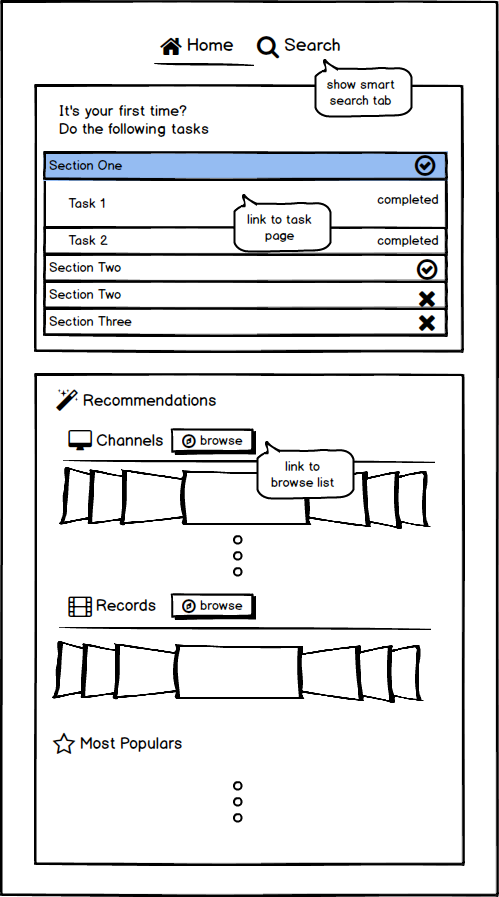
\includegraphics[width=0.8\textwidth]{mainPage.png}
	\caption{Dise�o de la p�gina principal}
	\label{fig:mainPage}
\end{figure}
En esta p�gina seg�n los requisitos debe existir un espacio para recomendaciones y otro para mostrar los contenidos m�s populares o votados. Por lo que esta va a se la estructura de la informaci�n de la p�gina. 
\paragraph{}
Adem�s incluiremos un \{\{navbarTab\}\} con las tabs Home y Search para acceder al contenido principal o al buscador como puede verse en la figura \ref{fig:mainPage}.
\paragraph{}
El contenido principal se estructura en tres bloques: 
\begin {itemize}
	\item \textbf{M�dulo de tareas iniciales:} este m�dulo impondr� al usuario una serie de tareas categorizadas que le ayudar�n a establecer un primer contacto con la aplicaci�n.
	\item \textbf{Relacionados:} este espacio estar� categorizado seg�n los tres grandes categor�as de contenido de la aplicaci�n (grabaciones,canales y lecciones). Los contenidos se mostrar�n como un carousel de miniaturas. Se mostrar�n los contenidos que compartan las tags que posean los contenidos votados por el usuario. De esta forma se oferta contenido relacionado a los gustos del usuario.
	\item \textbf{Populares:} aqu� se muestran los contenidos m�s populares del momento. Su representaci�n es id�ntica que la del espacio anterior.
\end{itemize}

\subsection{Sistema de b�squeda basado en modificadores}
Para hacer las b�squedas m�s r�pidas y precisas se ha implementado un sistema de b�squeda basado en modificadores. De manera que con solo introducir el car�cter + en el cuadro de b�squeda el sistema nos sugiera modificadores.
\paragraph{}
Los modificadores disponibles son: 
\begin{itemize}
	\item \textbf{+category: } los posibles valores son recordings, channels, lessons y all. Establece el tipo de contenido a buscar.
	\item \textbf{+author: } nos ir� sugiriendo usuarios mediante un auto-completado. Establece el autor de los contenidos.
	\item \textbf{+sort: } los posibles valores son latest y popular. Sirve para ordenar los resultados seg�n estos filtros.
	\item \textbf{+tag: } se trata de un auto-completado de etiquetas. Establece las etiquetas que poseer�n los resultados.
	\item \textbf{+from: } s�lo disponible cuando la categor�a corresponde a recordings. Los posibles valores son lesson o channel. Establecen la procedencia de las grabaciones a buscar.
	\item \textbf{+subscribed: } los valores son subscribed o unsubscribed. S�lo disponible si la categor�a corresponde a lessons o channels. Establece el estado de subscripci�n del usuario en los contenidos.
\end{itemize}
\paragraph{}
Los resultados se clasifican seg�n las categor�as en un sistema de tabs. Para cada categor�a se muestra el n�mero de resultados. 
\paragraph{}
La implementaci�n de este m�dulo integra una plantilla llamada \{\{<smartSearch\}\} que utiliza un objeto creado mediante el constructor SearchParamsManager creado en /app/client/lib/searchParamsManager.js. Dicho objeto se encarga traducir los actuales modificadores introducidos en par�metros de b�squeda o de subscripci�n para Mongo. Una vez traducidos procede a la subscripci�n de las publicaciones correspondientes. En este caso se han creado tres, una por categor�a y mediante el valor del modificador +category filtra las subscripciones. Adem�s se han creado plantillas de auto-completado para los modificadores y para la lista de sugerencias de cada uno.
\paragraph{}
La interfaz puede verse en la figura (tal).
\section{Prototipo 10: P�gina de inicio y m�dulos adicionales}
En este prototipo se ha implementado el apartado descriptivo de la aplicaci�n. Este comprende el desarrollo de la p�gina de inicio, los espacios para tutoriales y features y un m�dulo de ayuda. El resultado de esta implementaci�n puede verse en las figuras tal tal tal y tal.
\subsection{P�gina de inicio}
Se ha querido que la p�gina de inicio sea lo m�s descriptiva posible en lo que respecta a las caracter�sticas de la aplicaci�n y su funcionalidad. Por lo que se ha dise�ado en secciones. En cada secci�n se introducir� una caracter�stica y se mostrar� un enlace al recurso /features correspondiente a la misma. Tambi�n se ha creado una secci�n introductoria a los tutoriales con un enlace al recurso /tutorials.
\subsection{Espacio para tutoriales}
No es necesario que los usuarios est�n autenticados en el sitio para tener acceso a este espacio. Se ha creado un recurso /tutorials cuya layout es similar al principal. Est� formado por un sidebar y un header. El sidebar tiene s�lo un menu. El men� est� estructurado en secciones y cada secci�n contiene una lista de tutoriales. Los tutoriales ser�n videos que explicar�n c�mo realizar diversas funciones dentro de la aplicaci�n. Adem�s, para que sea m�s accesible, cada tutorial tendr� una url. Esto se ha hecho mediante query strings que indican la secci�n y el tutorial concreto que se desea visualizar. Se ha habilitado tambi�n un enlace en el sidebar de la aplicaci�n para acceder a este recurso en una nueva pesta�a.
\subsection{Espacio para features}
En este espacio se resumir�n todas las caracter�sticas y funcionalidades de la aplicaci�n. Al igual que para el espacio de tutoriales se crea un recurso /features que ser� accesible para todos los usuarios y el layout es id�ntico. Aunque el contenido var�a. El contenido de cada feature est� formado por una cabecera en la que aparece una imagen descriptiva y el t�tulo y un cuerpo en el que se muestra una galer�a de im�genes. Al hacer click en cada imagen podremos visualizarla en pantalla completa, leer su descripci�n y navegar por las que conforman la galer�a. Tambi�n se ha habilitado un enlace a este recurso en el sidebar de la aplicaci�n.
\subsection{M�dulo de ayuda flexible}
Este m�dulo est� formado por un bot�n y un collapsible de Bootstrap. Al hacer click en el bot�n se despliega una lista de preguntas frequentes que podemos editar y configurar v�a javascript para poder adaptar las preguntas al contexto de la p�gina en la que incluyamos dicho m�dulo. Cada pregunta es un enlace a uno de los tutoriales. 
\section{Prototipo Final: Notificaciones y restricciones de acceso}
En este prototipo se ha implementado el m�dulo de notificaciones y las plantillas \{\{notFound\}\} y \{\{accessDenied\}\}.
\subsection{Notificaciones}
Partiendo del requisito de que los usuarios deben estar informados en todo momento de cualquier cambio de su inter�s dentro de la aplicaci�n surge la entidad de Notificaciones y con ella la colecci�n Notifications (/app/lib/collections/notifications.js) cuyo objeto MongoDB ser� el mostrado en \ref{notificationMongo}.
\paragraph{}
Las notificaciones se visualizar�n en una pesta�a del sidebar como se muestra en la figura \ref{fig:sidebarNotifications}


Las notificaciones en el sidebar estar�n categorizadas por: canales, lecciones, grabaciones, conversations y contactos. Cada categor�a se mostrar� como un desplegable con la lista de las notificaciones correspondientes. �stas podr�n borrarse todas de una vez o independientemente. Al hacer click en cualquiera de ellas la aplicaci�n navegar� al contexto de la misma y la eliminar� de la base de datos. Puesto que es un contenido accesible en todo momento, incluiremos la subscripci�n a la publicaci�n que hemos desarrollado a la configuraci�n global de Iron Router:

\begin{lstlisting}[language=Javascript]
Router.configure({
	waitOn: function(){
		var subs = [
			Meteor.subscribe('conversationAlerts',Meteor.userId()),
			Meteor.subscribe('notifications',Meteor.userId())
		];
		return subs;
	}
})
\end{lstlisting}
\paragraph{} 
Para la creaci�n de las notificaciones se ha desarrollado el constructor NotificationsCreator (/app/client/lib/notificationsCreator.js) del cual se genera una instancia nada m�s arrancar el cliente. Este objeto posee el m�todo p�blico .createNotification que acepta los par�metros necesarios para su correcta creaci�n. Seg�n su tipo y su contexto generar� un mensaje distinto. 
\paragraph{}
Las notificaciones cubren la mayor�a de eventos en la aplicaci�n entre los que destacan: el voto a los contenidos, los comentarios, la creaci�n de contenido en canales y lecciones a los que el usuario se ha subscrito, cambios de usuarios en una conversaci�n, creaci�n de respuestas a grabaciones y peticiones de contacto.

\begin{figure}[htpb]
	\centering
	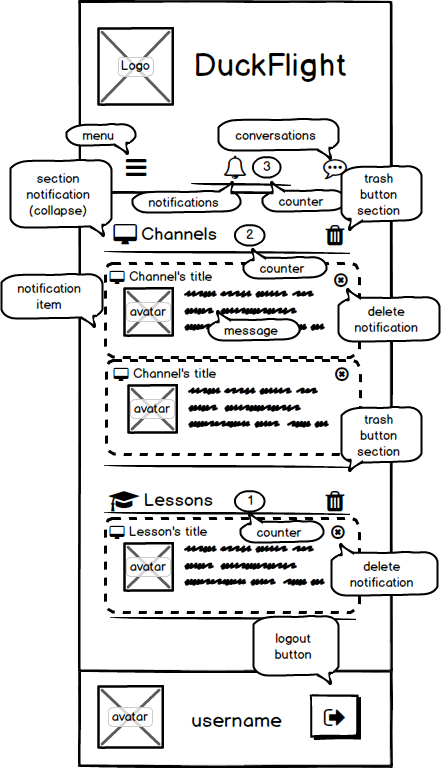
\includegraphics[width=0.7\textwidth]{sidebarNotifications.png}
	\caption{Dise�o de la pesta�a de notificaciones en el sidebar}
	\label{fig:sidebarNotifications}
\end{figure}

\subsection{Recursos de error}
\subsubsection{404}
El error 404 es devuelto por el servidor cuando los datos a los que intentamos acceder no existen. Esto puede deberse al acceso mediante url de alg�n recurso que ya no exista. Debe controlarse y se hace creando la plantilla \{\{$<$notFound\}\} (figura tal). Necesitamos utilizarla en dos posibles situaciones: 
\begin{itemize}
	\item El usuario accede a un recurso que cuyos datos han sido borrados, pero el recurso es v�lido.
	\item El usuario accede a un recurso inv�lido.
\end{itemize}
Los casos anteriores pueden ser controlados mediante Iron Router. El primero mediante el plugin 'dataNotFound' y el segundo mediante una nueva ruta colocada al final de todas las creadas y que acepte cualquier recurso. El siguiente c�digo ilustra la configuraci�n mencionada: 
\begin{lstlisting}[language=Javascript]
Router.plugin('dataNotFound',{template: 'notFound'});
Router.route('/(.*)',{name: 'notFound'});
\end{lstlisting}
\subsubsection{Access Denied}
Si bien la aplicaci�n no permite el acceso a contenidos privados para el usuario mediante el flujo dise�ado, si que es posible alterar las urls para navegar al recurso privado, por lo que esto debe de controlarse.
\paragraph{}
Para ello se ha creado la plantilla \{\{$<$accessDenied\}\} (figura tal), la cual se muestra cuando un usuario intenta editar alg�n recurso detalle del cual no es autor. Esto se consigue mediante los hooks de Iron Router, en concreto el hook beforeAction. He aqu� un ejemplo: 
\begin{lstlisting}[language=Javascript]
Router.route('/profile/:_id/edit',{
	...
	beforeAction: function(){
		if (Meteor.userId() !== this.params.id){
			this.render('accessDenied');
		}else{
			this.next();
		}
	}
});
\end{lstlisting}

\section{Despliegue}
El despliegue se ha llevado a cabo mediante el sistema de Hosting de Heroku. 

\subsection{Primeros pasos}
Para realizar este despliegue el primer paso ha sido crear una cuenta en heroku y descargar el CLI para poder desplegar nuestra aplicaci�n de forma remota. El despliegue en Heroku se basa en una idea muy simple. El despliegue es tan sencillo como almacenar una nueva versi�n de tu repositorio local en el repositorio remoto en github. El siguiente paso, una vez autenticado mediante el comando del CLI heroku login, creamos una aplicaci�n a la que damos el nombre de duckflight. Acto seguido nos devuelve dos urls que corresponden a dos repositorios remotos de github. Esa url la a�adiremos como repositorio remoto al actual.
\paragraph{}
Ahora necesitamos una base de datos remota, ya que hasta ahora hab�amos trabajado con la base de datos que nos creaba Meteor. Para ello creamos un sandbox en mlab mediante el CLI de heroku. Esto nos devolver� la url de la base de datos que deberemos atribuir como par�metro global a la aplicaci�n duckflight. 
\paragraph{}
Finalmente necesitamos un paquete constructor que se encargue de identificar que se trata de una aplicaci�n de Meteor y de generarla en la url en la que se har� el despliegue. Dicho paquete es jordansissel:heroku-buildpack-meteor y se configura mediante el comando heroku create --buildpack <buildpack>. 
\paragraph{}
Una vez seguidos estos pasos, procedemos al despliegue de la aplicaci�n mediante el comando git push heroku master.
\subsection{Proceso}
En el momento que ejecutamos el comando anterior se crea una copia de nuestro repositorio local en el repositorio remoto heroku. Acto seguido el buildpack o paquete constructor se encarga de generar nuestra aplicaci�n y de arrancarla en la url correspondiente.
\subsection{Pruebas globales}
Una vez realizado el despliegue se han llevado ha explotado la funcionalidad de la aplicaci�n de forma que se han probado todas las caracter�sticas de la misma. El resultado de estas pruebas ha sido satisfactorio.

\chapter{Pruebas de Validaci�n}
En este cap�tulo se representa la fase de experimentaci�n del proyecto. Esta fase se basa en la realizaci�n de una prueba en la que se ha medido la utilidad de la aplicaci�n y su rendimiento en un entorno real.
\section{Motivaci�n}
La principal motivaci�n de este experimento es analizar el comportamiento de la aplicaci�n en la realidad. Dicho comportamiento deber� cumplir estrictamente los requisitos propuestos en la secci�n \ref{sec:requisitos}.
\section{Planteamiento y objetivos}
Una vez desplegada la aplicaci�n en Heroku \cite{baz14} y realizadas las pruebas globales oportunas se ha procedido a generar contenido en la misma y a plantear el experimento. 
\paragraph{}
El experimento consistir� en hacer accesible la aplicaci�n a un grupo de alumnos mediante la difusi�n de la url donde ha sido alojada. Dichos alumnos, siguiendo la gu�a de uso elaborada para esta fase del proyecto, explotar�n todas las caracter�sticas de la aplicaci�n y su funcionalidad. Por otra parte se ha integrado a la aplicaci�n el servicio de Google Analytics \footnote{\url{https://analytics.google.com}} para controlar y analizar el flujo de usuarios dentro de la aplicaci�n.
\paragraph{}
Los objetivos perseguidos se han resumido en las siguientes caracter�sticas:
\begin{itemize}
	\item \textbf{Funcional:} la aplicaci�n debe cumplir todos los requisitos establecidos.
	\item \textbf{Atractiva e intuitiva:} que los alumnos aprecien el atractivo de las interfaces y el flujo de la aplicaci�n.
	\item \textbf{Fluida y �ptima:} la aplicaci�n debe comportarse de manera fluida con m�s de un usuario utiliz�ndola.
	\item \textbf{�til:} la aplicaci�n debe suponer una herramienta de trabajo para los alumnos. 
\end{itemize}
\paragraph{}
Para medir y analizar el cumplimiento de los objetivos marcados se ha desarrollado una encuesta o formulario que se ha difundido junto con la gu�a de uso. Los alumnos, una vez completada la gu�a, aportar�n informaci�n sobre su experiencia contestando a las preguntas de dicho formulario.
\section{Proceso y realizaci�n}
El proceso y la realizaci�n ha sido muy sencilla, Se han habilitado los recursos necesarios (gu�a y formulario) de forma remota y se ha procedido al env�o de dichos enlaces a un grupo de alumnos.
\section{Resultados y an�lisis}
Una vez que los alumnos han probado la aplicaci�n y han rellenado la encuesta se ha procedido al an�lisis de los resultados. 
\chapter{Conclusi�n}
\phantomsection
%% cite example: \cite{baz1}%%
\addcontentsline{toc}{chapter}{\bibname}
\begin{thebibliography}{99}
	\bibitem{baz1} P�gina oficial WebRTC: \url{https://webrtc.org/}
	\bibitem{baz2} P�gina para WebRTC experiments (recordRTC): \url{https://www.webrtc-experiment.com/RecordRTC/}
	\bibitem{AceEditor} P�gina oficial de AceEditor: \url{https://ace.c9.io/}
	\bibitem{AceEditorPackage} Paquete AceEditor para Meteor: \url{https://github.com/mizzao/meteor-sharejs}
	\bibitem{baz3} P�gina oficial SoundCloud: \url{https://soundcloud.com}
	\bibitem{baz4} P�gina para desarrolladores SoundCloud: \url{https://developers.soundcloud.com/}
	\bibitem{baz5} P�gina oficial MeteorJS: \url{https://www.meteor.com/}
	\bibitem{baz6} Gu�a de MeteorJS: \url{http://guide.meteor.com/}
	\bibitem{baz7} Documentaci�n de MeteorJS: \url{http://docs.meteor.com/#/full/}
	\bibitem{bazMongoDB} P�gina oficial de MongoDB: \url{https://www.mongodb.com/es}
	\bibitem{baz8} P�gina oficial Bootstrap: \url{http://getbootstrap.com/}
	\bibitem{baz9} W3C javascript tutorial: \url{http://www.w3schools.com/js/}
	\bibitem{baz10} Documentaci�n de MongoDB: \url{https://docs.mongodb.com/manual/}
	\bibitem{baz11} P�gina oficial JQuery: \url{https://jquery.com/}
	\bibitem{baz12} Documentaci�n de JQuery: \url{http://api.jquery.com/}
	\bibitem{baz13} Documentaci�n de UnderscoreJS: \url{http://underscorejs.org/}
	\bibitem{bazIronRouter} Repositorio de Iron Router en Github: \url{https://github.com/iron-meteor/iron-router}
	\bibitem{baz14} Despliegue en Heroku: \url{https:duckflight.herokuapp.com/}
	\bibitem{bazGitRepo} C�digo fuente del proyecto: \url{https://github.com/jortegamo/duckflight}
	\bibitem{bazWikiProyect} Wiki del proyecto: \url{https://github.com/jortegamo/duckflight/wiki}
	\bibitem{bazWikiTutoriales} Documentaci�n del producto: \url{https://github.com/jortegamo/duckflight/wiki/Video-Tutoriales}
	\bibitem{bazHeroku} Tutorial para el despliegue: \url{http://justmeteor.com/blog/deploy-to-production-on-heroku/}
	\end{thebibliography}

\appendix
\clearpage 
\addappheadtotoc
\appendixpage
\chapter{Dise�o de la base de datos y documentos para MongoDB}
En este ap�ndice se muestra el esquema Entidad Relaci�n y los objetos BSON dise�ados para cada una de las entidades.
\label{appendix:documentsdesign}
\begin{figure}[htpb]
	\centering
	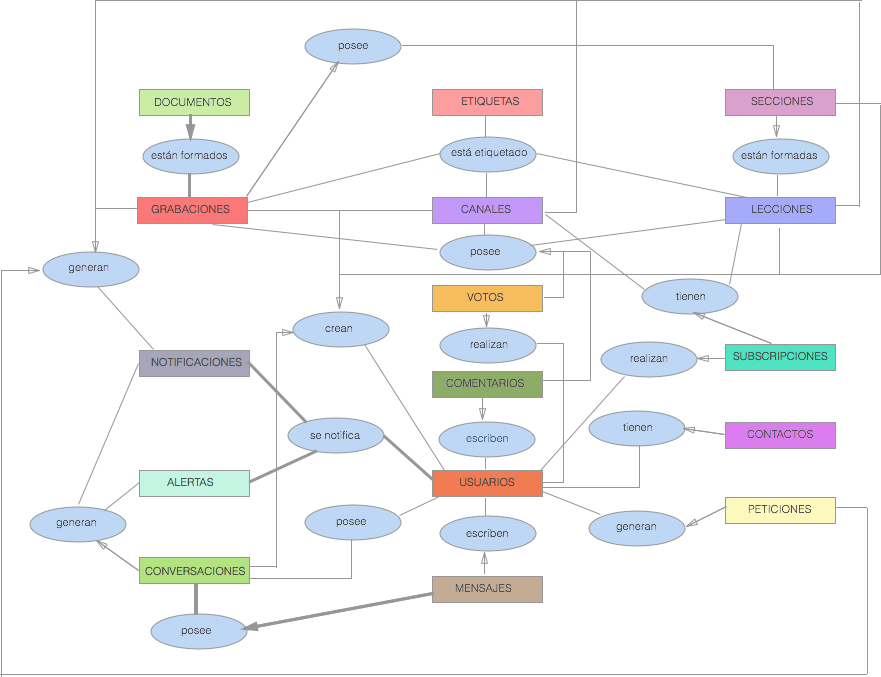
\includegraphics[width=0.9\textwidth]{ERdesign.png}
	\caption{Esquema entidad relaci�n}
	\label{fig:ERdesign}
\end{figure}
\vspace{1cm}
\begin{lstlisting}[language=javascript, caption=Dise�o de documento para una grabaci�n, label={recordMongo}]
var record = {
    _id: //idMongo,
    author: //idUser,
    title: //no �nico,
    description: //(opcional),
    RC: [{},...], //Funciones de reproducci�n sobre el editor
    createAt: //fechaCreaci�n,
    docs_count: //contador de documentos,
    votes_count: //contador de votos,
    replies_count: //contador de respuestas,
    comments_count: //contador de comentarios,
    channel_id: //canal al que pertenece,
    lesson_id: //lecci�n a la que pertenece,
    section_id: //secci�n a la que pertenece dentro de una lecci�n,
    order: ,//orden dentro de la lista de reproducci�n.
    tags: [{},...], //etiquetas,
    ready: //(boolean) para conocer la disponibilidad del record.
    img: //imagen miniatura,
    duration: //duraci�n en milisegundos de la grabaci�n.
    isReply: //(boolean) indica si se trata de una respuesta a otro record.
    parent_id: //idMongo del record al que responde.
    track: //{_id: 'id del track en SoundCloud', link: 'link SoundCloud'}
}; 
\end{lstlisting}
\vspace{1cm}
\begin{lstlisting}[caption=Dise�o de documento para los documentos de cada grabaci�n, label={documentMongo}]
var doc = {
    _id: //idMongo,
    record: //record al que pertenecen,
    doc: {
         title: //titulo del documento (�nico para el record),
         theme: //tema del editor tras �ltimo cambio,
         mode: //tema del editor tras el �ltimo cambio,
         value: //�ltimo estado del contenido del editor
    },
    start: //(boolean) (True)? comienzo grabaci�n : se ha creado durante la grabaci�n
           //o es el estado final de otro inicial.
};

\end{lstlisting}
\vspace{1cm}
\begin{lstlisting}[caption=Dise�o de documento para un canal, label={channelMongo}]
var channel = {
    _id: //idMongo,
    author: //id_user,
    title: //�nico,
    banner: //url img banner,
    img: //url img miniatura,
    description: //(opcional),
    tags: //etiquetas [{name: //nombre etiqueta}],
    createAt: //fechaCreaci�n,
    votes_count: //contador para los votos,
    records_count: //contador para los records,
    comments_count: //contador para los comentarios,
    users_count: //contador para los usuarios que se subscriban
};
\end{lstlisting}
\vspace{1cm}
\begin{lstlisting}[caption=Dise�o de documento para una lecci�n, label={lessonMongo}]
var lesson = {
    _id: //idMongo,
    author: //id_user,
    title: //�nico,
    img: //url img miniatura,
    description: //(opcional),
    tags: //etiquetas [{name: //nombre etiqueta}],
    createAt: //fechaCreaci�n,
    votes_count: //contador para los votos,
    sections_count: //contador para las secciones,
    comments_count: //contador para los comentarios,
    users_count: //contador para los usuarios que se apunten
}; 
\end{lstlisting}
\vspace{1cm}
\begin{lstlisting}[caption=Dise�o de documento para una secci�n, label={sectionMongo}]
var section = {
    _id: //idMongo,
    title: //�nico,
    createAt: //fechaCreaci�n,
    records_count: //contador para los records,
    lesson_id: //id de la lecci�n a la que pertenece.
    order: //orden de la secci�n.
}; 
\end{lstlisting}
\vspace{1cm}		
\begin{lstlisting}[caption=Dise�o de documento para cada subscripci�n de un usuario, label={userEnrolledMongo}]
var userEnrolled = {
    _id: //idMongo,
    contextId: //id del canal o de la lecci�n a la que se han subscrito,
    user_id: //id del usuario
};
\end{lstlisting}
\vspace{1cm}
\begin{lstlisting}[caption=Dise�o de documento para una etiqueta, label={tagMongo}]
var tag = {
    _id: //idMongo,
    name: //nombre para la etiqueta
};
\end{lstlisting}
\vspace{1cm}
\begin{lstlisting}[caption=Dise�o de documento para una conversaci�n, label={conversationMongo}]
var conversation = {
    _id: //idMongo,
    subject: //asunto de la conversaci�n,
    author: //l�der de la conversaci�n.
    last_modified: //fecha de ultima modificaci�n (cada vez que se inserta un mensaje),
    members: //[{},...], array de miembros,
    members_count: //contador para los miembros,
    messages_count: //contador para los mensajes
};
\end{lstlisting}
\vspace{1cm}
\begin{lstlisting}[caption=Dise�o de documento para los mensajes, label={messageMongo}]
var message = {
    _id: //idMongo,
    author: //id del creador,
    createdAt: //fecha de creaci�n,
    message: //contenido del mensaje
    conversation_id: //id de la conversaci�n a la que pertenece.
}
\end{lstlisting}
\vspace{1cm}
\begin{lstlisting}[caption=Dise�o de documento para una alerta de conversaci�n, label={conversationAlertMongo}]
var conversationAlert = {
    _id: //idMongo,
    user_id: //usuario al que se le muestra la alerta,
    conversation_id: //id de la conversaci�n de la que procede,
    alertsAllow: //flag (boolean) si es true se muestran las alertas y si es false no.
    alerts_count: //contador de alertas
};
\end{lstlisting}
\vspace{1cm}
\begin{lstlisting}[caption=Dise�o de documento para cada usuario, label={userMongo}]
var user = {
    _id: //idMongo,
    username: //nombre de usuario (�nico),
    avatar: //avatar del usuario,
    banner: //banner de la pagina de usuario,
    description: //descripci�n del usuario,
    status: //estado de conexi�n,
    emails: //[{address: //emailAddress,verified: //Boolean,},...],
    ... //otros campos establecidos por meteor-accounts.
};
\end{lstlisting}
\vspace{1cm}
\begin{lstlisting}[caption=Dise�o de documento para las peticiones de contacto, label={requestsMongo}]
var request = {
    _id: //idMongo,
    requested: //{id: id_user, delete: boolean},
    applicant: //{id: id_user, delete: boolean},
    status: //(string) 'pending', 'accepted', 'refused'
};
\end{lstlisting}
\vspace{1cm}
\begin{lstlisting}[caption=Dise�o de documento para establecer la relaci�n de contacto, label={relationMongo}]
var relation = {
    _id: //idMongo,
    createdAt: //fecha creaci�n,
    users: //[id_user_requested, id_user_applicant],
};
\end{lstlisting}
\vspace{1cm}
\begin{lstlisting}[caption=Dise�o de documento para los comentarios, label={commentMongo}]
var comment = {
    _id: //idMongo,
    author: //id del creador,
    createdAt: //fecha de creaci�n,
    isReply: //(Boolean) indica si es una respuesta o no,
    replies_count: //contador de respuestas,
    message: //contenido del mensaje
};
\end{lstlisting}
\vspace{1cm}
\begin{lstlisting}[caption=Dise�o de documento para una notificaci�n, label={notificationMongo}]
var notification = {
    _id: //idMongo,
    to: //id_user destinatario,
    from: //id_user origen,
    parentContextTitle: //es el t�tulo de la lecci�n, record o channel en el que se ha producido,
    urlParameters: //son los par�metros para construir el enlace al clickar sobre la notificaci�n,
    type: //(string) 'channel', 'record', 'comment', etc,
    message: //(string) de contenido HTML
};
\end{lstlisting}










\end{document}  


